\documentclass[12pt]{article} % JASA requires 12 pt font for manuscripts
%\usepackage{JASA_manu}        % For JASA manuscript formatting

\usepackage{times, asa, url}
\RequirePackage{pdf14}
%\usepackage{endfloat} % just for while I am writing

% for citations
\usepackage[authoryear]{natbib} % natbib required for JASA
\usepackage[colorlinks=true, citecolor=blue, linkcolor=blue]{hyperref}

% for the fancy tables with the icons
%\usepackage[margin=1.0in]{geometry}% http://ctan.org/pkg/margin
\usepackage{booktabs}% http://ctan.org/pkg/booktabs
\usepackage{array}% http://ctan.org/pkg/array
\newcolumntype{M}{>{\centering\arraybackslash}m{\dimexpr.05\linewidth-2\tabcolsep}}


%\definecolor{Blue}{rgb}{0,0,0.5}
\usepackage[usenames,dvipsnames]{xcolor}
\newcommand{\hh}[1]{{\color{orange} #1}}
\newcommand{\al}[1]{{\color{ForestGreen} #1}}

%% For printing in black and white
%\newcommand{\hh}[1]{{\color{black} #1}}
%\newcommand{\al}[1]{{\color{black} #1}}

% fonts
%\usepackage{kpfonts}

% for figures
\usepackage{graphicx}
\DeclareGraphicsExtensions{.eps, .pdf}
\graphicspath{{figures/}}

% help with editing and coauthoring
\usepackage{todonotes}
\newcommand{\alnote}[1]{\todo[inline,color=green!40]{#1}} %% nice template!!
\newcommand{\hhnote}[1]{\todo[inline,color=orange!40]{#1}} 
\newcommand{\dcnote}[1]{\todo[inline,color=blue!40]{#1}} 

% title formatting
%\usepackage[compact,small]{titlesec}

% page formatting
\usepackage[margin = 1in]{geometry}
%\usepackage[parfill]{parskip}

% line spacing
\usepackage{setspace}
\doublespace

% For math typsetting
\usepackage{bm}
\usepackage{amstext}
\usepackage{amssymb}
\usepackage{amsmath}
\usepackage{amsfonts}
\usepackage{multirow}

% A few commands to make typing less tedious
\newcommand{\inv}{\ensuremath{^{-1}}}
\newcommand{\ginv}{\ensuremath{^{-}}}
\newcommand{\trans}{\ensuremath{^\prime}}
\newcommand{\E}{\ensuremath{\mathrm{E}}}
\newcommand{\var}{\ensuremath{\mathrm{Var}}}
\newcommand{\cov}{\ensuremath{\mathrm{Cov}}}

\renewcommand{\textfraction}{0}
\renewcommand{\bottomfraction}{1}
\renewcommand{\topfraction}{1}
\renewcommand{\floatpagefraction}{1}


\title{Better Diagnostics for Linear Mixed-Effects Models Using Visual Inference}

\author{{Adam Loy, Heike Hofmann, Dianne Cook}
\thanks{Adam Loy is an Assistant Professor (e-mail: adam.m.loy@lawrence.edu) in the Department of Mathematics, Lawrence University, Appleton, WI 54911. Heike Hofmann is a Professor in the Department of Statistics and Statistical Laboratory, Iowa State University, Ames, IA 50011. Dianne Cook is a Professor in the Department of Statistics and Statistical Laboratory, Iowa State University, Ames, IA 50011.}}


\begin{document}
\maketitle

\begin{abstract}
 Valid model-based statistical inference relies on proper specification of a model, making diagnostic tools central to analysis. Graphical methods are commonly used for checking the assumptions of a model; however, they are often criticized as being too subjective since decisions are based on one plot. This has lead to the reliance on conventional hypothesis tests to make formal decisions. Recently, visual inference has been established, providing a rigorous framework for graphical discovery that allows for the quantification of strength of evidence. In this paper we use visual inference as a framework to overcome common difficulties with conventional hypothesis tests and statistical graphics that are encountered in the selection and validation of linear mixed-effects models. Additionally, we compare three versions of Quantile-Quantile plots with respect to power. \dcnote{Abstracts get changed at last stage of writing so maybe not ready to edit yet. Needs to be more specific: what is the problem with diagnostics for linear mixed-effects models?}
\keywords{Statistical graphics; Lineup protocol; Visual tests; Model diagnostics;  ...}
\end{abstract}

%\tableofcontents
%------------------------------------------------------------------------------------
\section{Introduction}
%------------------------------------------------------------------------------------
%\hhnote{We need a good motivating examples early on. Pushing figure 1 to the front might be a solution -- we need to capture the attention right away. Maybe the first cyclone plot is even better, as there's no actual solution in form of a test available. We can then come back to this example throughout the intro of visual inference and the general discussion. It'll help in making the discussion more concrete.}

Linear mixed-effects models are versatile models that account for dependence structures when data are composed of groups.
%---such data structures are especially common in social science research where studies often focus on responses from human subjects. 
Such structures occur, for example, when individuals are naturally grouped by organization (e.g., students within schools), geography (e.g., voters within states), or design (e.g., respondents assigned to  interviewers). The additional flexibility offered by these models allows data to be incorporated at both the observation-level (level 1) and the group-level (level 2, or higher) while also accommodating dependencies between individuals within the same group. 

For data organized in $g$ groups, consider a continuous response linear mixed-effects model (LME model) for each group $i$, $i=1, \ldots, g$:
%
\begin{equation}\label{eq:hlm}
	\underset{(n_i \times 1)}{\bm{y}_i} = \underset{(n_i \times p)}{\bm{X}_i} \ \underset{(p \times 1)}{\bm{\beta}} + \underset{(n_i \times q)}{\bm{Z}_i} \ \underset{(q \times 1)}{\bm{b}_i} + \underset{(n_i \times 1)}{\bm{\varepsilon}_i}
\end{equation}
%
where $\bm{y}_i$ is the vector of outcomes for the $n_i$ level-1 units in group $i$, $\bm{X}_i$ and $\bm{Z}_i$ are design matrices for the fixed and random effects, respectively, $\bm{\beta}$ is a vector of $p$ fixed effects governing the global mean structure, $\bm{b}_i$ is a vector of $q$ random effects describing the between-group covariance structure, and $\bm{\varepsilon}_i$ is a vector of level-1 error terms accounting for the within-group covariance structure. The random effects,  $\bm{b}_i$,  are assumed to be a random sample from $\mathcal{N}(\bm{0},\ \bm{D})$ and independent from the level-1 error terms,  $\bm{\varepsilon}_i$, for which are assumed to follow a distribution of $\mathcal{N}(\bm{0},\sigma^2 \bm{I}_{n_i})$. %\bm{R}_i)$. 
Here, $\bm{D}$ is a positive-definite $q \times q$ covariance matrix and $\bm{I}_{n_i}$ denotes the $n_i \times n_i$ identity matrix.
Finally, it is assumed that all between group effects have a covariance of zero.

Inference typically centers around either the marginal or conditional distribution of $\bm{y}_i$, depending on whether global or group-specific questions are of interest.
Based on model \eqref{eq:hlm} the marginal distribution of $\bm{y}_i$ for all $i = 1, \ldots, g$ is given by
%
\begin{equation}\label{eq:marginalmod}
\bm{y}_i \sim \mathcal{N}\left(\bm{X}_i\bm{\beta},\ \bm{V}_i \right),
\end{equation}
%
where $\bm{V}_i = \bm{Z}_i \bm{DZ}_i\trans + \sigma^2 \bm{I}_{n_i}$, and the conditional distribution of $\bm{y}_i$ given $\bm{b}_i$ is defined as
%
\begin{equation}\label{eq:conditionalmod}
\bm{y}_i | \bm{b}_i \sim \mathcal{N}\left(\bm{X}_i\bm{\beta} + \bm{Z}_i \bm{b}_i, \ \sigma^2 \bm{I}_{n_i} \right).
\end{equation}
%


Residuals are central to the exploration of a linear mixed-effects model, similar to the classical linear model with uncorrelated error structure. For linear mixed-effects models, residual analysis is complicated by the fact that there are numerous quantities that can be defined as \emph{residuals}, with each residual quantity being associated with different aspects of the model. The two fundamental residuals for model checking considered here are:
%
\begin{itemize}
\item the \emph{level-1 (observation-level) residuals}, ~the conditional residuals or error terms: $\widehat{\bm{\varepsilon}}_i = \bm{y}_i - \bm{X}_i \widehat{\bm{\beta}} - \bm{Z}_i \widehat{\bm{b}}_i$,

\item and the \emph{level-2 (group-level) residuals}, ~the predicted random effects $\widehat{\bm{b}}_i$
\end{itemize}
%
where $\widehat{\bm{\beta}}$ is an estimate of the fixed effects, % (for known $\bm{V}$),
\begin{equation}\label{eq:glsb}
	\widehat{\bm{\beta}} = 
	\left(\sum^g_{i=1} \bm{X}\trans_i \bm{V}^{-1}_i \bm{X}_i \right)^{-1} 
	\sum^g_{i=1} \bm{X}_i\trans \bm{V}_i\inv \bm{y}_i,
\end{equation}
and $\widehat{\bm{b}}_i$ are predictions of the random effects, given as
\begin{equation}\label{eq:eb}
	\widehat{\bm{b}}_i = \bm{D} \bm{Z}_i\trans \bm{V}_i^{-1} 
	\left(\bm{y}_i - \bm{X}_i \widehat{\bm{\beta}} \right), \ \ \ \ \forall\ i = 1, \ldots, g.
\end{equation}
%
When $\bm{V}_i$ is unknown, estimates for the covariance matrices are used in the above equations. These estimates are commonly found through maximum likelihood (ML) or restricted maximum likelihood (REML). %

%\alnote{If we use subheadings in the intro, then we need one here. I don't have a good idea for one right now... Maybe ``purpose'' or something since this is where we really outline what we're going to do and why.}
%\subsection{Issues with model exploration and diagnostics}

The additional flexibility of random effects models comes at the cost of complicating model exploration and validation. %For example:
%\hh{In this paper we want to address some of these situations and offer validated graphical diagnostics as solutions:}
Problems addressed in this paper are:


\begin{enumerate}
\item {\em Model selection:}
\begin{enumerate}
\item {\em Breakdown of  asymptotic results:} Test statistics used for model selection and validation rely on asymptotic reference distributions which often perform poorly in finite sample situations. 
For example, the empirical distribution of the predicted random effects  does not resemble the theoretical distribution unless strong assumptions are met \citep[Theorem 3.2 and Lemma 3.1]{Jiang:1998vt}. In many finite sample situations these assumptions do not hold, making conventional use of Q-Q plots and tests of the empirical distribution function ineffective for distributional assessment \cite[see the supplement of][for supporting simulation results]{adam}.

\item {\em Boundary issues  in the comparison of nested models: } 
When evaluating the significance of terms in the random effects structure, the likelihood ratio test statistic does not have the usual $\chi^2$ reference distribution if we are testing whether a variance component lies on the boundary of the parameter space. This results in tests for the random effects that tend to be conservative.
%\cite{Stram:1994wd} argue that using the usual $\chi^2$ reference distribution leads to conservative results, and suggest using a 50:50 mixture of $\chi^2_q$ and $\chi^2_{q+1}$ when testing $q$ versus $q + 1$ random effects; however, this adjustment is not successful in all cases.}

%\item[Incomparability  of nested models due to estimation procedure: ]
% Comparison of nested models with different fixed effects not possible with REML estimation, too liberal for ML. 
\end{enumerate}


\item {\em Model checking:} Residual plots might display noticeable patterns that are artifacts of both the data structure and the model estimation procedure rather than indications of lack of fit. 
This problem is especially pronounced for  scatterplots comparing predicted random effects. Such plots can display points falling along a line that is oriented in conflict with the estimated correlation between the random effects \cite[see][for an example]{Morrell:2000ve}. 
%\hhnote{XXX I'm not quite sure how that would look like}.  
%\alnote{This would look like a scatterplot with the slope oriented in the wrong direction (i.e., in conflict with the estimated correlation from ML or REML). I haven't encountered this in practice, but it is what Morrell and Brant talk about.}
Additionally,  plots of the error terms often exhibit patterns that appear to be indicative of heteroscedasticity, but are merely consequences of data imbalances or sparsity.

\end{enumerate}

The above issues are well-known, and in special circumstances adjustments to the methodology have been proposed. For example, \cite{Stram:1994wd} suggest using a 50:50 mixture of $\chi^2_q$ and $\chi^2_{q+1}$ when testing $q$ versus $q + 1$ random effects; however, this adjustment is not successful in all cases.  \cite{Lange:1989uu} suggest using weighted Q-Q plots to assess the distributional assumptions made on the random effects. This approach is effective in settings where the residual variance, $\sigma^2$, is small relative to the variance components for the random effects, but breaks down when this is not the case \citep{adam}.
 

%\hh{Why are you going back to lineups now? - it might be better to shift this sentence back by a couple of paragraphs}
%Lineups for visual inference heavily rely on the types of residuals defined above. %Next, we compare conventional and visual inference for model selection and validation.
%Below we discuss methods commonly used to check the validity of the assumptions made on model \eqref{eq:hlm} using the level-1 and -2 residuals.


The purpose of this paper is to illustrate the use of visual inference for diagnosing LME model fits, and propose graphical tests that can be broadly used in situations where the assumptions of conventional inferential procedures are violated. This approach allows us to harness the power of graphical diagnostics and, with the rigor of the visual inference framework, construct tests that address some of these problems without requiring additional assumptions. 


The remainder of this paper is organized as follows. 
Section~\ref{sec:vi} provides an introduction to the framework of visual inference and the lineup protocol. Sections~\ref{sec:select} and \ref{sec:checking} expand on the problems encountered in model selection and model checking, respectively, and solutions utilizing visual inference. 
%In Section~\ref{sec:checking} we present graphical tests for model validation. 
Throughout both sections multiple examples are used, and comparisons between conclusions on model building and fit from the new visual inference approach and existing diagnostic tools are provided. All example data sets are readily available for public use. A short description of each data set can be found in Appendix~\ref{sec:datasets}.

%\alnote{Should we include another pointer to the descriptions of the data sets?}
%\hhnote{Usually contents of the appendices aren't discussed in the introduction - but we need to extend the description of the paper a little bit more, you're right with that!}

%We also show results of a study investigating the power of three different versions of the familiar Q-Q plot. 

%\todo[inline]{paragraph on the structure of the paper:  next section deals with visual inference in the framework of hierarchical models, and suggests a series of visual tests as alternative to tests that in the classical setting don't work too well because of easily violated assumptions or nature of the setup. Then we will discuss using power to choose specific designs in the evaluation of distributional assumptions in the familiar graphical setting of the Q-Q plots. }



%%------------------------------------------------------------------------------------
\section{Visual inference}\label{sec:vi}
%%------------------------------------------------------------------------------------
%In order to develop graphical model diagnostics as substitutes for statistical tests of model assumptions, we must work within a rigorous inferential framework. 
%\cite{Gelman:2004gg} formulates a visual analog of simulation-based model diagnostics in which a visualization of an aspect of the model is compared to data generated under the model. \cite{Buja:2009hp} extend this idea, proposing two protocols that formalize a rigorous inferential framework for testing visual discoveries. In this section we outline the lineup protocol.

Classical statistical inference consists of 
(i) formulating  null and alternative hypotheses,
	(ii) calculating a test statistic from the observed data,
	(iii) comparing the test statistic to a reference (null) distribution,
	and (iv) deriving a $p$-value on which a conclusion is based.
Each of these steps has a direct analog in visual inference, as outlined by \cite{Buja:2009hp}. 
%As we will apply visual inference in the setting of linear mixed-effects models, 
We will highlight  parallels between conventional hypothesis tests and visual inference in the setting of linear mixed-effects models.
%in this setting. 

Assume that  the question of interest involves  some assumption about a model (such as a null hypothesis of homogeneity of residual variance) while the alternative hypothesis  encompasses any violation of this model assumption. 
%e.g.~let us assume that the null hypothesis is  homogeneity of residual variance,
%while
%the alternative hypothesis encompasses any violation of this model assumption. 
For visual inference, the test statistic corresponds to a plot  that displays an aspect of  the model assumption and allows the observer to distinguish between scenarios under the null hypothesis from scenarios under alternative hypotheses. 
Plots drawn from data generated consistently with the null hypothesis are called \emph{null plots}. The set of all null plots constitutes the reference distribution; thus, the plot of the observed data is indistinguishable from the null plots if the model assumption holds.
%If the model assumption holds, the plot of the observed data is indistinguishable from the null plots. 
In the lineup protocol the plot of the observed data is randomly embedded
 among a sample of, usually 19, null plots drawn from the reference distribution.  These \emph{lineups} are then presented to independent observers for evaluation. 

Evaluation by independent observers  allows for the estimation of a $p$-value associated with the lineup.
 Let $X$ be the random variable describing  the number  of observers, out of $N$, identifying the data plot. 
If $X=x$ is  the number of observers who chose the data plot from the lineup, then the  $p$-value is  the probability that at least $x$ observers choose the data plot, given that the null hypothesis  is true (i.e.~the  data plot is not any different from the other plots in the lineup). Under the null hypothesis the probability of choosing the true plot is $1/m$ (for a lineup of size $m$), and $X$ is distributed according to a distribution similar to a Binomial distribution $B_{N, 1/m}$, but adjusted for the dependencies between plots in a given lineup.
%inherent to the application of lineups in a human subject study 
(\citet{mahbub:2013} introduced visual $p$-values. Details of their calculation for this LME application are in Appendix~\ref{sec:pvalues}.)
%\alnote{I am debating whether we need a reference to the appendix at the end of the last sentence... but I haven't made a decision yet.}

%with a probability of success of $p = 1/m$\al{---that is,}  $X~\sim~B_{N, p}$. The $p$-value \hh{for this lineup} is then estimated as
%\begin{equation}\label{eqn.pvalue}
%\widehat{p\text{-value}} = P(X \ge x) = \sum_{k= x}^N {N \choose k} \left(1/m\right)^k \left(1 - 1/m\right)^{N-k}.
%\end{equation}
%\hhnote{this is just the $p$ value conditioned on the lineup. For the unconditioned $p$ value we need to `integrate' the effect of the lineup out - we have multiple samples of null sets for the same data. We need to still write out how to combine those.}
\begin{figure}
	\centering
	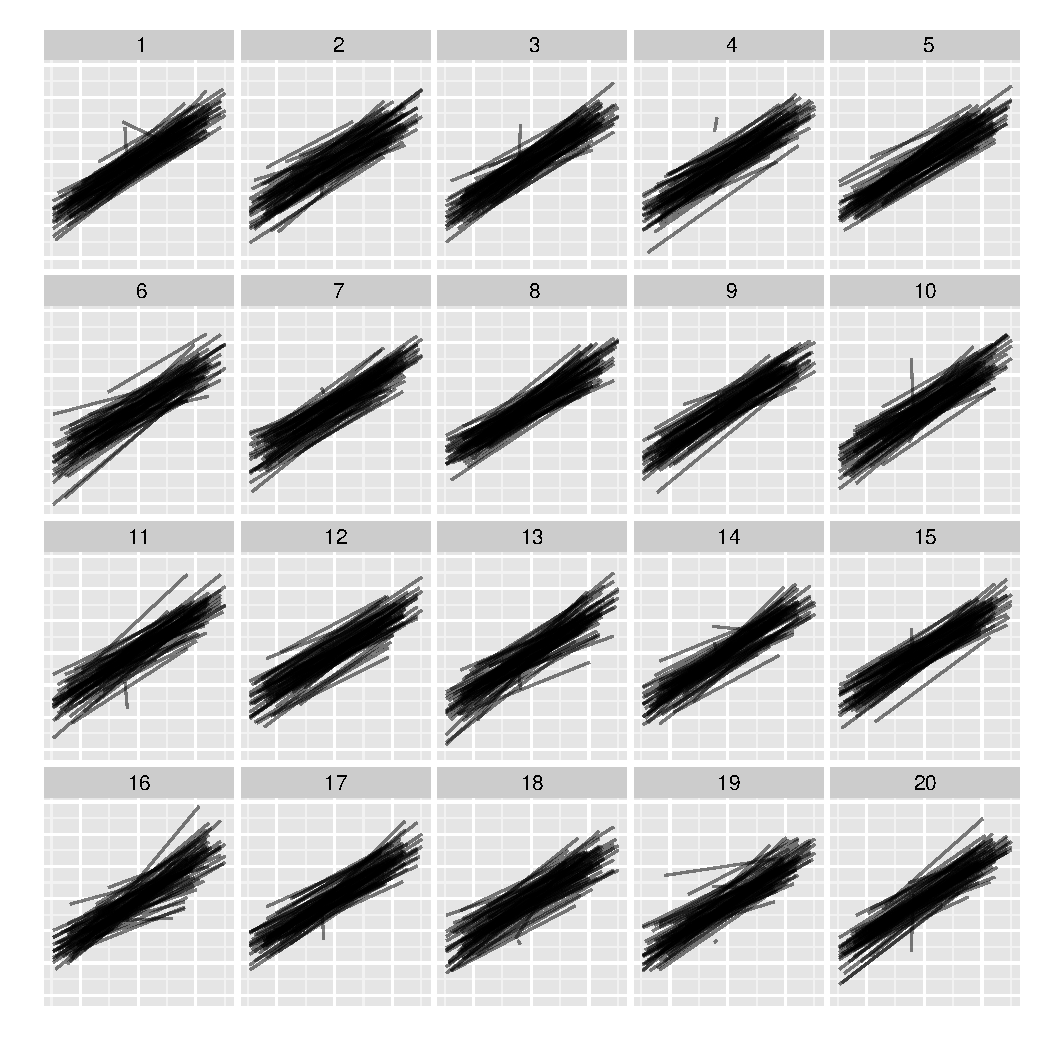
\includegraphics[width=0.8\textwidth]{normexam_fanned_lineup16.pdf}
	\caption{\label{fig:fanned} A lineup of size 20. Which plot is the most different from the other plots? What makes that plot different from the other plots?
	}
\end{figure}

Figure~\ref{fig:fanned} shows a lineup. Each panel shows  line segments of different lengths  with varying slopes. Observers were asked the question `Which plot is the most different?'.    Any  information revealing the context of the data, such as axis labels, units, titles, and legends,  was carefully removed to  avoid subjective bias \citep{meilgaard}, ensuring observers from make decisions that were based purely on the data display. 
%\alnote{Reading J's comments on my dissertation, this is where he asked about more information on the observers. At this point we could point ahead to where we discuss the study further or include a brief explanation of Amazon MTurk to address this comment.}

Based on a human subject study (described in more detail in Appendix~\ref{study}) run through the Amazon MTurk service \citep{amazon}, 11 out of 73 observers  chose the  data plot, shown in panel  \#($\sqrt{144} + 4$) of the lineup in Figure~\ref{fig:fanned}, resulting in a visual $p$-value of 0.0171. This leads us to reject the null hypothesis that the data plot %is consistent with the null model with a $p$-value of  0.0171. The actual model of the data and the null hypothesis are explained in detail in Section~\ref{sec:select}. 
is consistent with the model that generated the data, on which all of the other plots are based. The  model and its corresponding null hypothesis  are explained in detail in Section~\ref{sec:select} .  


Unlike classical hypothesis tests, visual inference  allows us to collect additional information on what aspect of the display led each observer to their choice. 
%Rather than to just reject a null hypothesis 
This  information makes it possible us assess which part of the null hypothesis is violated, something not feasible in classical hypothesis tests. For example,  `Spread' as the reason for an observer's choice (over `Outlier', `Trend',  `Asymmetry', or `Other') in Figure~\ref{fig:fanned} was associated with the highest probability of picking the data over a null plot (see Table~\ref{tab:reasons}).

%\alnote{The sentence below needs some rewording}
%In the example of the first lineup of figure~\ref{fig:fanned} `spread' as the reason for their choice increased observers' chances to pick the data over a null plot. 
%\hhnote{Should we give the reasons for the first example?}
%\alnote{That's a good idea. I think we can give both the common choices from MTurk, and our own analysis of the plot, since it is possible to get both from a lineup.}

%\subsection{Model notation and formulation} 
%------------------------------------------------------------------------------------


%------------------------------------------------------------------------------------
\section{Model selection}\label{sec:select}
%------------------------------------------------------------------------------------

\noindent
%The lineup protocol presents a unified approach to overcome the difficulties encountered when checking the validity of a hierarchical linear model. The only change necessary to utilize this approach to model checking is the generation of null plots, for which we use the parametric bootstrap. Consequently, the ``standard'' residuals plots can be used within this framework in order to overcome the subjectiveness of interpretation and identification of artificial structures, making visual inference a natural extension of conventional model checking. 
%In this section we discuss several examples of lineups that we have found useful for model checking; however, we do not intend to present an exhaustive overview.

%In this section we discuss how visual inference can be used during model selection.

%One statistical model is nested within another when the \emph{larger model} contains all components included in the \emph{smaller model}
%% with respect to both fixed and random effects, 
% as well as some additional component(s). For example, the larger model may include additional fixed effects, or include additional random effects. Two models are not nested when one model cannot be viewed as a special case of the other. For example, if two models contain different sets of fixed effects.
 Model selection for linear mixed-effects models relies on the comparison of nested models for the selection of both the fixed and random components. 
% To select fixed effects $t$- and $F$-tests are commonly used, while likelihood ratio tests are used to select the random effects. 
% \hh{For comparing non-nested models we usually make use of  AIC or BIC  \citep{anderson1998}.}
% In this section we discuss how to use visual inference as a unified testing framework for model selection of both fixed and random effects.
 % for both nested and non-nested models. 
%\subsubsection{Conventional practices}
%\subsection{Comparing nested models}\label{sec:select-fixed}
%------------------------------------------------------------------------------------
%\alnote{This paragraph is a lot of repeat from the last paragraph, other than the intro to complications. I need to think about ways to resolve this.}
It is standard practice to use a $t$-test, $F$-test, or likelihood ratio test to determine whether a fixed effect describes a significant portion of the unexplained variability. % in a linear mixed-effects model. 
%Likelihood ratio tests are more generally applicable in comparing nested models, but are  most commonly used in the selection of random effects. 
For selecting random effects likelihood ratio tests are most commonly used. 
%One statistical model is nested within another when the \emph{larger model} contains all components included in the \emph{smaller model}, with respect to both fixed and random effects, as well as some additional component(s). For example, the larger model could differ by including additional fixed effects, or by including additional random effects. 
%While statistical software has made performing many of these tests easy, 
However, situations often arise that complicate such tests. 
%Below we outline such situations.
Some of these are outlined below:

\begin{description}
\item[\bf Fixed effects: ] Likelihood ratio tests based on REML estimation cannot be used to test different fixed effects structures. Maximum likelihood estimation allows for such comparisons, but is anti-conservative. 
Defining the appropriate degrees of freedom in using  $t$- or $F$-tests provide another  complication in testing scenarios of LME models. Various approximate $F$-tests \citep{Verbeke:2000fh} propose solutions for estimating the degrees of freedom for these tests, but these typically lead to different results. Inflated Type I error rates and low power \citep{Catellier:2000vr}  become a problem  in the  approximate $F$-test when there are a few groups. \cite{Kenward:1997ft} propose the use of a scaled Wald statistic  that has a sampling distribution that is well approximated by an $F$ distribution; however, this approach has inflated type I error rates in some small sample cases  \citep{Gomez:2005dw}. \cite{Skene:2010kf} propose an alternative to the Kenward-Roger approximation that achieves nominal type I error rates, but this procedure suffers from low power. 
%From the literature it can be seen that tests for fixed effects are not always problematic, but they are complicated by the number of special cases that must be considered.
%XXX Need to reread the below references to check accuracy of these summaries:
%
%\cite{Kenward:1997ft} propose the use of a scaled Wald statistic that has a sampling distribution that is well approximated by an $F$ distribution 
%
%Problems with Kenward and Roger's method: has inflated type I error rates for some small sample cases  \citep{Gomez:2005dw}
%
%An alternative to the Kenward-Roger approximation that achieves nominal type I error rates but have low power \citep{Skene:2010kf}.


%\alnote{I could also mention the messy business of defining the degrees of freedom here.}
%\hhnote{yes, a bit of that discussion would be good. I'm not sure that we can cite Bates - but maybe by now he's actually published something on that discussion, which is the main reason for his aversion of putting in p values.}
%\alnote{I am taking a look through the literature. I did find Bates' ``rant'' (which is quite hilarious and interesting) \url{https://stat.ethz.ch/pipermail/r-help/2006-May/094765.html}, and I also found a paper by Hodges that might be applicable, but I need to read it to make that determination:
%
%Hodges, J. S., \& Sargent, D. J. (2001). Counting degrees of freedom in hierarchical and other richly-parameterised models. \emph{Biometrika}, 88(2), 367--379.
%}
\item[\bf Random components: ] When testing for the inclusion of a variance component, the parameter being tested lies on the boundary of the parameter space, and the asymptotic distribution of the likelihood ratio is no longer a $\chi^2$ distribution. Approximations have been suggested and shown to be useful in many situations \citep{Stram:1994wd, Morrell:1998ua}, but no single approximation holds for all situations. This leads to a need for simulation studies to determine the proper adjustment to the reference distribution in every situation. Alternatively, the rule of thumb suggested by \citeauthor{Stram:1994wd} can be utilized with the knowledge that the results may be sub-optimal, leading to either conservative or anti-conservative decisions. 
\end{description}


Visual inference provides an alternative to conventional hypothesis tests that does not require different rules based on the method of estimation or location of a parameter in the parameter space, and avoids the tricky business of defining degrees of freedom. Rather, visual inference depends on the choice of an appropriate plot highlighting the aspect of the model in question, the number of null plots, and the number of independent observers. Below we discuss how visual inference can be utilized to test the significance of fixed and random effects.

\subsection{Fixed effects} 
To test the significance of a fixed effect, we suggest using a plot comparing a residual quantity from the model without the variable of interest with the values of that variable. 
The residual used depends on the level at which the variable of interest enters the model: if the variable enters at the observation-level (level-1), then the level-1 residuals are used; if the variable enters at the group level, then both the level-1 and level-2 residuals are explored as the variable has the potential to explain additional variation at either level of the model.
Additionally, the type of plot depends on the variable type---if a continuous variable is targeted,  a scatterplot with a smoother is suitable for testing; for a discrete covariate, we make use of side-by-side box plots. 
In this setting, the null plots are generated using the parametric bootstrap  with a model that omits the variable of interest. The true plot is constructed from the same model but uses the observed data. 

\begin{figure}[h]
	\centering
	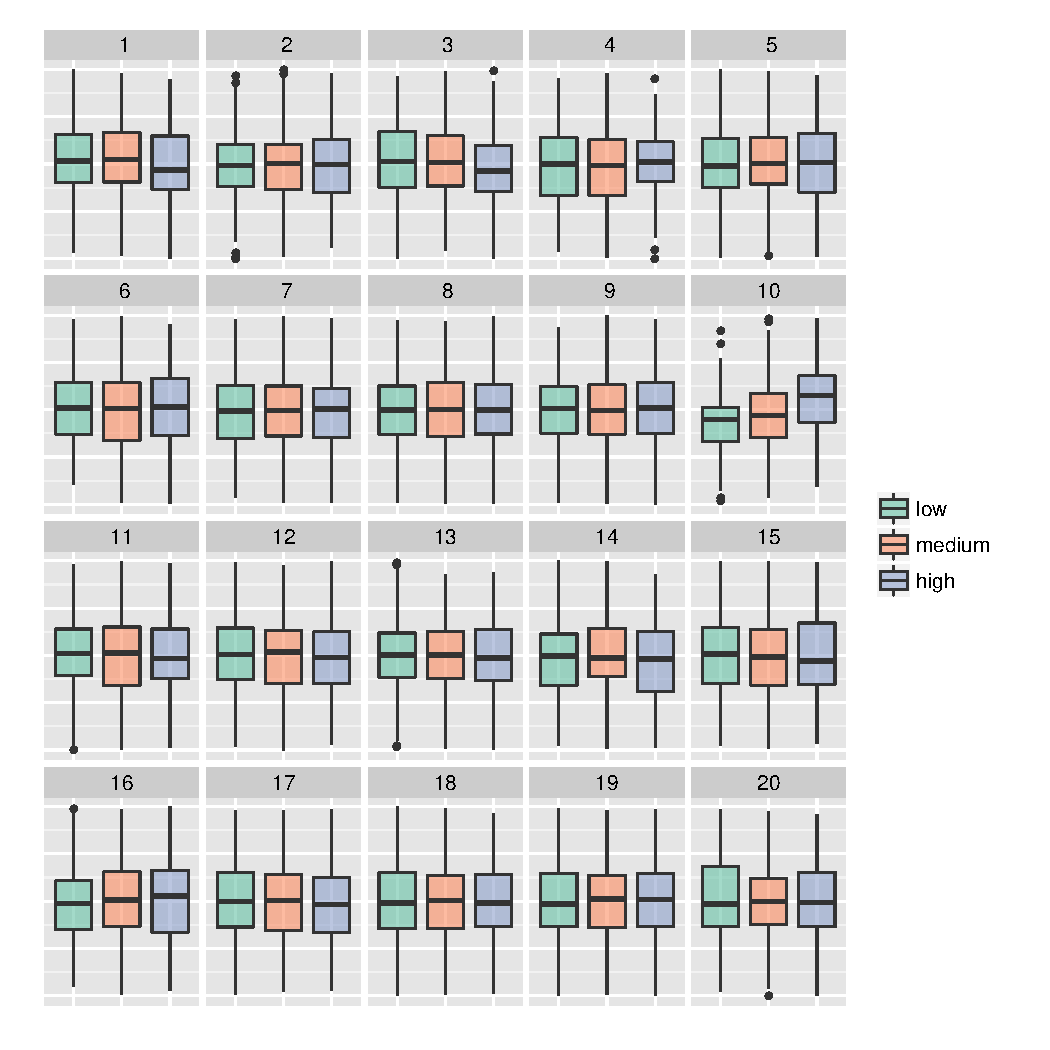
\includegraphics[width=0.8\textwidth]{autism2-ordered-10.pdf}
	\caption{\label{fig:boxplot-ordered} {Lineup of level-1 residuals in box plots  by groups to test significance of a discrete covariate.}
%	\todo[inline]{I'm starting to get nitpicky again :)
%	The legend is added (to make the point later that it doesn't help much with the overall pattern), the boxes are a bit transparent (maybe alpha of 0.6?) so the gridlines in the back don't completely disappear and we need to use a different color scheme - the red and the green are not color blind safe. } 
%	\todo[inline]{Why did you decide to remove the outliers? Are you worried the outliers distract from the pattern? - We could test that!}
%	\alnote{That is why I removed the outliers. It would be interesting to test.}
	Which of the plots is the most different? Which feature led you to your choice?} 
\end{figure}

Figure~\ref{fig:boxplot-ordered} illustrates the use of this type of lineup. In our study, 74 observers were asked to choose the plot that is the most different from the rest. Sixty five observers identified the data plot in panel \#($2^3 + 2$), 
%corresponding to a $p$-value of XXX, 
with 40.3\% pointing to the trend as the distinguishing feature. 
This lineup is chosen
to determine whether a child's language development at age two (low, medium, or high) helps explain the development of social skills from childhood to adolescence for children diagnosed with autism spectrum disorder (see Appendix~\ref{data:autism} for details on the data and analysis). Displayed on the $y$-axis are level-1 residuals from a longitudinal model. Clearly, language development at age two accounts for a significant amount of the remaining residual variability.
%The underlying data are level-1 residuals from a longitudinal 
%Lineup testing for the significance of social skills (low, medium, or high) for a longitudinal model investigating investigating the development of social skills from childhood to adolescence for children diagnosed with autism spectrum disorder. Here the level-1 residuals are used to see if the variable accounts for any additional residual variability. 


%\begin{figure}
%	\hfill
%	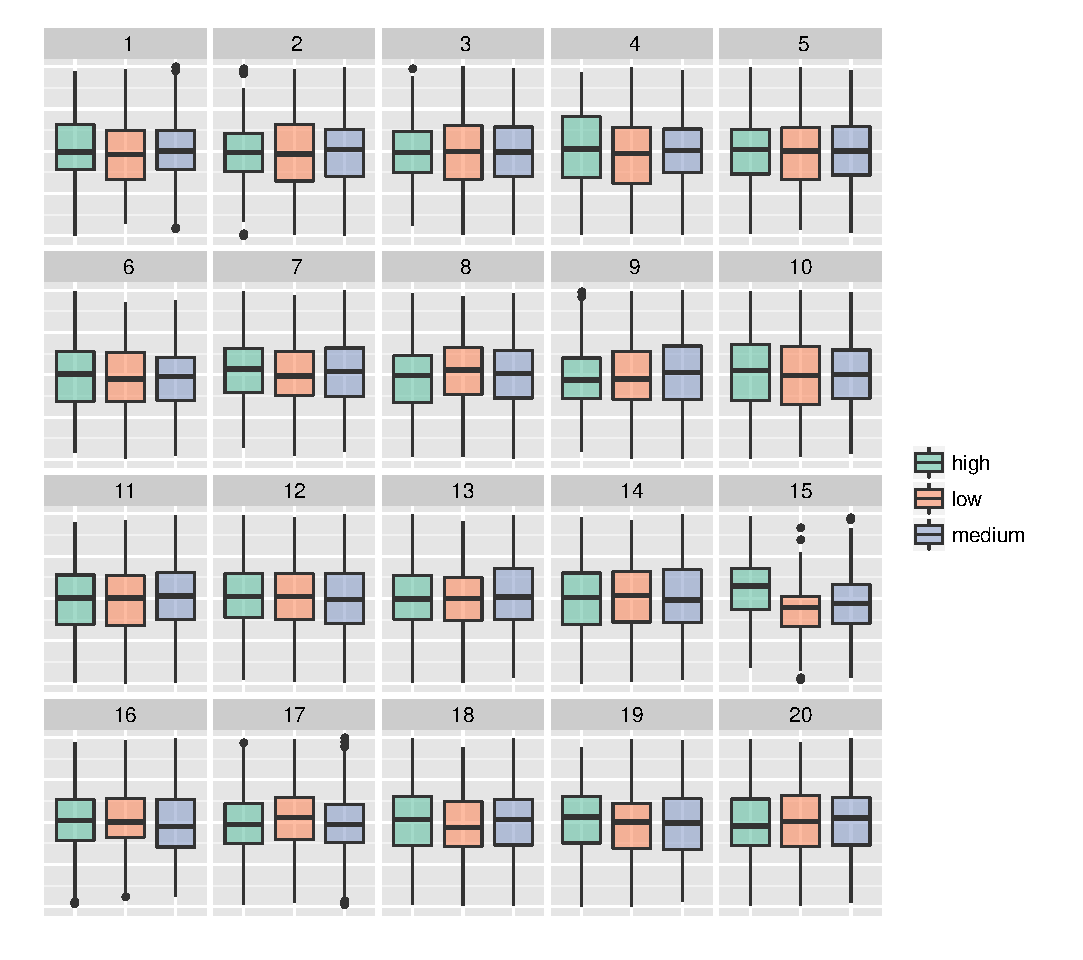
\includegraphics[width=0.9\textwidth]{autism_sicdegp_level1_lineup4.pdf}
%	\caption{\label{fig:boxplot-unordered} Lineup testing for the significance of social skills (low, medium, or high) for a longitudinal model investigating investigating the development of social skills from childhood to adolescence for children diagnosed with autism spectrum disorder. Here the level-1 residuals are used to see if the variable accounts for any additional residual variability. Which is the real plot?}
%\end{figure}


\subsection{Random effects}\label{sec:random}
Tests of the random part of a linear mixed-effects model focus on two questions: (1) whether a marginal random effect improves the model and (2) whether allowing the random effects to be correlated improves the model. Different plots must be used to answer each question. To answer the first question, we suggest using plots comparing the response and the explanatory variable of interest using appropriate (often linear) smoothers for each group. Scatterplots comparing the predicted random effects can be used to answer the second question.

The lineup in Figure~\ref{fig:fanned} was chosen to test the relationship between scores from the General Certificate of Secondary Education Exam (GCSEE) and the  standardized London Reading Test (LRT) (see Appendix~\ref{data:GCSE} for details).  Each line segment represents one of 65 inner-London schools. The slope of each line is determined by a linear regression relating the two test scores for all students at a school. 
The question of interest is whether random slopes for LRT scores are required to  represent the relationship between GCSEE and LRT scores ($H_1$). Correspondingly, data for the null plots  were  created by simulating GCSEE scores from a model with only a single random effect, the random intercept.
The resulting scores for each school are regressed on LRT results and shown as lines.
%\al{and overlaying linear smoothers for each school.}
%Revisiting Figure~\ref{fig:fanned} we see an example of testing for the inclusion of a random effect. Recall that the initial model was a random intercept model using a student's score on the standardized London Reading Test to describe their age 16 score on the General Certificate of Secondary Education examination.
 %To construct this figure we used the parametric bootstrap to generate simulated GCSEE exam scores, fit separate regression models to the simulated responses, and then plotted the fitted model for each school. 
 If the model is appropriate, then the overall pattern of the lines in the null plots should resemble the observed data. In this example, we find that the true plot in panel \#($\sqrt{144} + 4$) is identifiable:  11 of the 73 observers pick the data plot, resulting in a visual $p$-value of 0.0171. The main comments participants gave to explain their choice were the spread and trend of the line segments in the plot. This is consistent with a larger variance of slopes than the null model allows;
  %GCSEE scores   for higher scores on the standardized LRT than \hh{accommodated for} in the null plots; 
  thus, we find evidence supporting the inclusion of a random slope for standardized LRT. This conclusion agrees with the results of the likelihood ratio test (which shows significance at a level of less than 0.0001), and did not require the use of an asymptotic distribution to calculate the $p$-value. 
%\alnote{The p-value is $<$ 1e-4.}
  
\begin{figure}
	\centering
	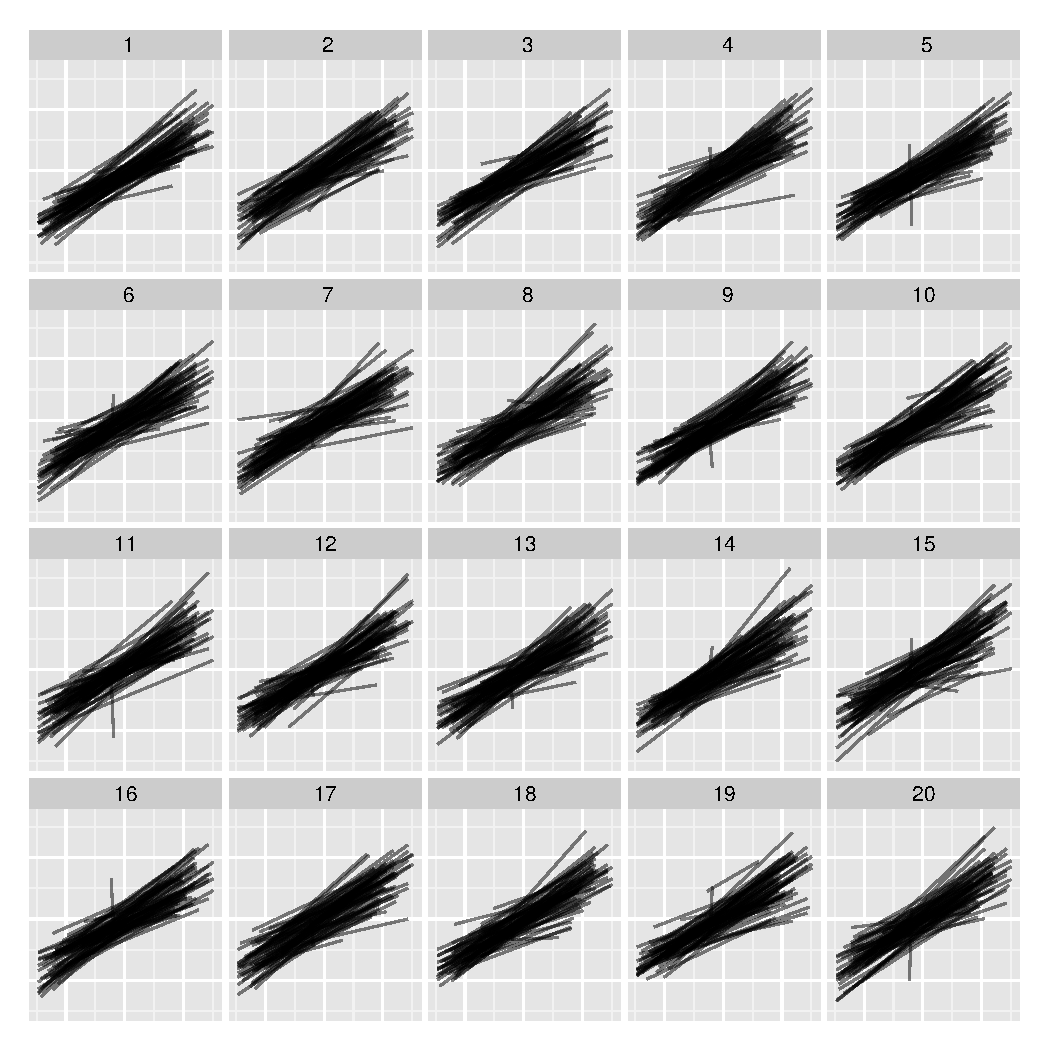
\includegraphics[width = 0.8\textwidth]{normexam_fanned_withslope_lineup18}
	\caption{\label{fig:fanned2} A follow-up to Figure~\ref{fig:fanned} where the random slope has been included in the model. Which plot is the most different of the others?}
\end{figure}

%\alnote{We should consider talking about the need for another lineup here. Originally, we only included one lineup to save space, but in practice we would need two: the first lineup associated with the original model in question, and a second to see if the addition of the random slope was enough. This was also brought up by Di during my defense.}
%\hhnote{yes, I agree - we actually need another lineup on this for the new experiment ***LINEUP***(added to folder) I would suggest to include the random slope in the model from which you simulate the null and draw the same picture again. Hopefully the data disappears.}
%\alnote{Here is a lineup with the random slope. Can you find the data?\\[1em]
%
%A similar thing can be done with the trajectories plotted for the autism data, should we do include that one too?}
%\hhnote{I like this figure! I know which panel it is - by now I recognize the data, but Christian couldn't tell. Is the code included in lineups-study2.R?}

{Note that participants are unable to identify the true data from a follow-up lineup (Figure~\ref{fig:fanned2}) where the random slope was included in the model.
%showing lines stemming from regression fits of null data from a model including the random slope.  
All panels show data from the same distribution and the true data should therefore not be identifiable.  None of the 64 observers identified the data plot in panel \#$(2\cdot 3^2)$. }

%\hhnote{XXX what else would you like to say about this lineup test? -- we could talk about how this supports the validity of the lineup protocol: it picks up on actual differences and does not when we are dealing with a case where the data is consistent with the null hypothesis. }
%\alnote{I think that is a good idea!}

Participants should only see one of Figures~\ref{fig:fanned} or~\ref{fig:fanned2} because both show the same data, even in the same design. After viewing the first of these figures we cannot, strictly speaking, assume that a participant is still an unbiased judge, because theoretically the data from the  second lineup could be identified by recognizing it as the same panel that was previously shown. While the chance of this is slim in practice, we only exposed participants to one of a set of dependent lineups.
%ensured in the user study to expose participants to only one of a set of of dependent lineups.  

Having considered the value of a random slope in the model, we next consider whether the model needs to allow the random effects to be correlated ($H_1$). While this is an example of a standard likelihood ratio test problem---a correlation of zero is not on the boundary of the parameter space---using a lineup keeps all tests of the random effects in a unified framework. The lineup in Figure~\ref{fig:ranef-corr} shows scatterplots of the predicted random effects with overlaid regression lines. 
%This type of plot is suggested by  \cite{Morrell:2000ve} as a visual diagnostic for assessing the amount of correlation. 
 The null plots in the lineup are created by simulation from the model that does not allow for correlation between the random effects, and the true plot is created using the predicted random effects from such a model fit to the observed data.
The slopes of the regression lines are indicative of the amount of correlation. 
%Note that with a higher amount of shrinkage in the random effects we start to see more lines with a higher amount of slope. 
 If the correlation between the random effects is not necessary, then the true plot will display little correlation and be indistinguishable from the null plots.
The lineup allows us to gauge the amount of correlation between the random effects while accounting for the effect of shrinkage in the model, avoiding the over-interpretation of structure in such plots discussed by \cite{Morrell:2000ve}.
  In Figure~\ref{fig:ranef-corr} the true plot in panel~\#($10 + \sqrt{25}$) was identified by 41 of the 69 observers, providing very strong evidence in  support of  the additional parameter for correlation between random effects, which agrees with a $p$-value of 0.0041 from the classical likelihood ratio test.
%  \hhnote{What does the $p$-value of the classical LRT say?}
%  \alnote{The $p$-value from the classical LRT is 0.0041, agreeing with our conclusion.}

\begin{figure}[hbt]
	\centering
	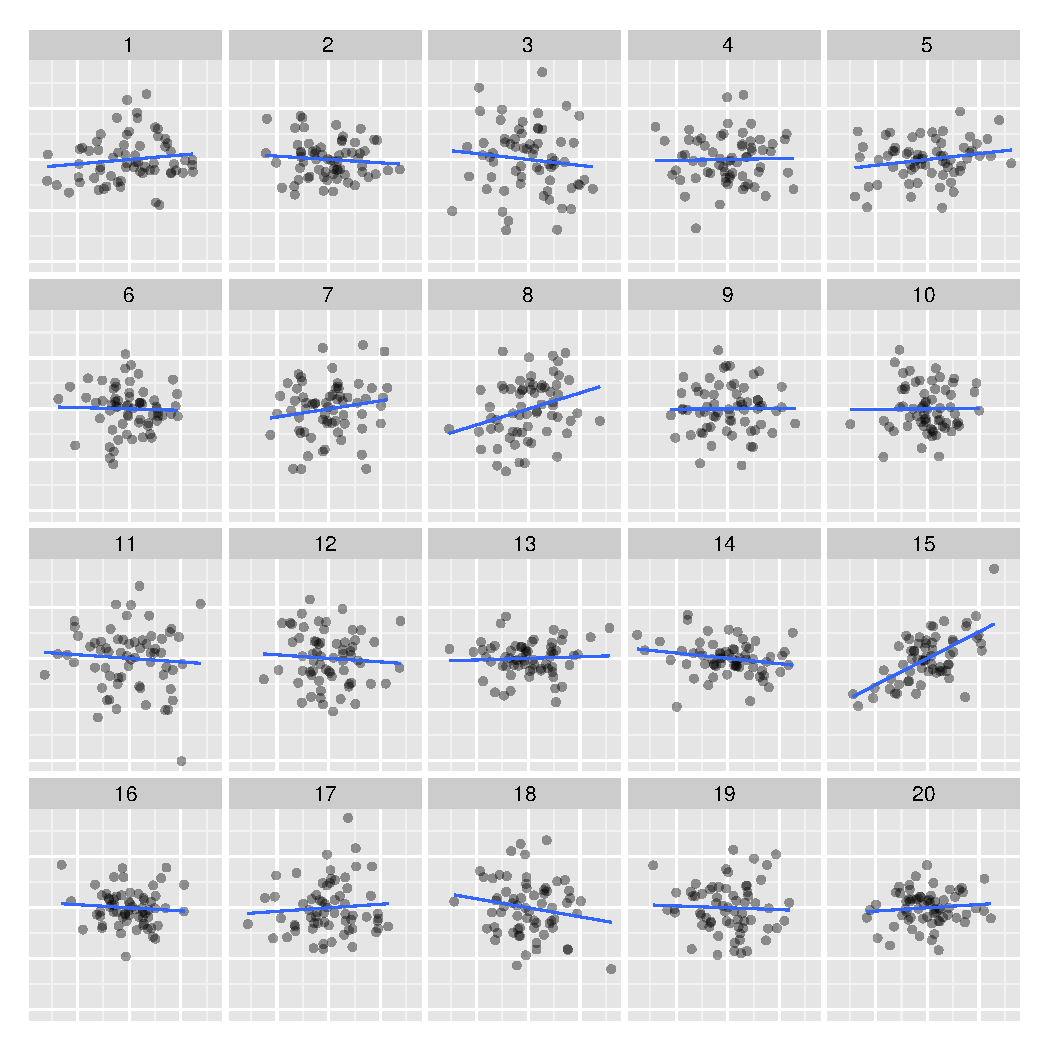
\includegraphics[width=0.8\textwidth]{examcorr-15.pdf}
	\caption{\label{fig:ranef-corr} Lineup for testing the correlation between random effects. Which plot is the most different of the others? What feature in the panel led you to your choice?}
\end{figure}

%\alnote{We could move the negative lineups that we did not include in the study to the appendix. I am thinking about this more from the perspective of when we submit to a journal with length restrictions}
%
%\begin{figure}
%	\centering
%	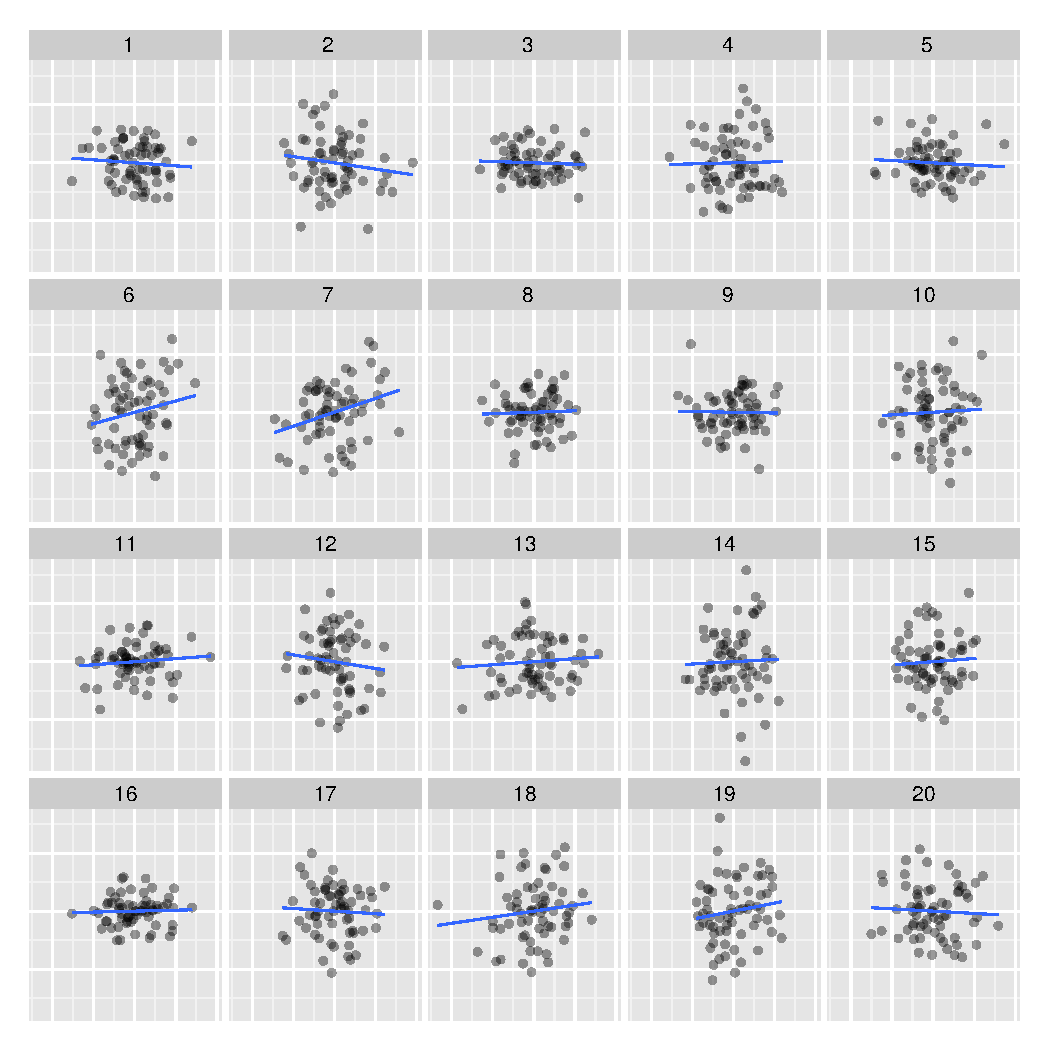
\includegraphics[width=\textwidth]{normexam_uncorr_lineup13.pdf}
%	\caption{\label{fig:ranef-uncorr}  Lineup testing the need to allow for correlation between the two random effects. These 20 plots compare the predicted random intercept and slope for the model fit to the Exam data. Which is the real plot?}
%\end{figure}


%\todo[inline]{Make the following paragraph a bullet list. This will help to emphasize the important parts. At the moment they get lost a bit.
%\begin{description}
%\item[\bf Fixed effects in nested models: ] likelihood ratio tests based on REML estimation do not allow for testing different fixed effect structures. Maximum likelihood estimation allows for it, but is conservative. 
%\item[\bf Random components in nested models: ] likelihood ratio tests for random components suffer from boundary effects. 
%\end{description}}

%Statistical software has made performing $t$-tests for fixed effects simple, but more thought is often required when performing a likelihood ratio test. More specifically, likelihood ratio tests can only be used with nested models fit by REML if they differ only with respect to their random components. This is because the restricted log likelihood contains a term that changes with $\bm{X}_i$ \citep[c.f.,][Section 2.2.5]{Pinhiero:2000vf}. Nested models fit by ML do not have this restriction, so likelihood ratio tests can be used to test both the fixed and random effects. 
%Additional complications arise in the computation of a $p$-value for the likelihood ratio test for covariance parameters on the boundary of the parameter space. In this case, the asymptotic reference distribution is not $\chi^2$ with degrees of freedom equal to the difference in the number of parameters. \cite{Stram:1994wd} suggest the use of a 50:50 mixture of $\chi^2$ distributions with $q$ and $q + 1$ degrees of freedom when testing $q$ versus $q + 1$ random effects. While this approximation has been shown to be useful \citep{Morrell:1998ua}, it does not apply to every case.  We refer the reader \citet[Section 2.4.1]{Pinhiero:2000vf} for an example of when a this approximation is not successful. The lack of a general rule for approximating the distribution of the likelihood ratio test statistic reveals the need for a more transparent procedure for determining whether a random effect should be included in the model.


%\subsection{Comparing non-nested models}
%%------------------------------------------------------------------------------------
%If two models are not nested, then the likelihood ratio test cannot be used to determine the preferred model. In this case, it is conventional practice to use the Akaike Information Criterion (AIC) as an index enabling model comparison, where the model with the smaller AIC is preferred. While AIC provides a concise and convenient way to compare non-nested models, it is only an index and does not address whether the model with the smaller AIC is significantly ``better'' than the other. To do this, we propose using lineups to investigate the goodness-of-fit of each model. If inadequacies are discovered in one model but not in the other, then this supports the use of the properly specified model. This approach is similar in concept to comparing the AIC from each model, but by focusing on an investigation of how the true data depart from the assumptions made by the model we can see why a model is preferred.
%%
%\hhnote{Do we have a lineup for this, or an idea of how to do a lineup checking for the goodness of fit?}
%\alnote{No, we don't have a lineup for this. I added this in the original manuscript ``to be complete,'' but I think that it could be omitted. It doesn't add much and length could be an issue.}

%\subsubsection{Proposals for visual inference}\label{model-selection}
%------------------------------------------------------------------------------------

%Visual inference provides an alternative to conventional hypothesis tests that does not have limitations based on whether ML or REML was used to fit the model since it does not rely on the (restricted) log likelihood. Additionally, the $p$-value from a visual test is calculated using the Binomial distribution, which does not require adjustments to an asymptotic distribution. Rather, visual inference depends on the plot chosen, the number of alternatives, and the number of viewers. Below we discuss plots for visual inference useful in model selection.

%\paragraph{Fixed effects.} To test the significance of a fixed effect, we suggest using a plot comparing a residual quantity from the model without the variable of interest and the values of that variable. The residual that should be used depends on the level at which the variable of interest enters the model---if the variable enters at the observation-level (level-1), then the level-1 residuals should be used; if the variable enters at the group level, then both the level-1 and level-2 residuals should be explored as additional variation at either level could be explained by this variable. Additionally, the type of plot depends on the variable type---if a continuous variable is targeted,  a scatterplot with a smoother \hh{is suitable for testing}; for a discrete covariate, \hh{we can make use of} side-by-side boxplots. 
%
%
%In this setting, the null plots are generated using the parametric bootstrap with a model that omits the variable of interest. The true plot is constructed from the same model but using the observed data. Figure~\ref{fig:boxplot-ordered} illustrates the use of this type of lineup to determine whether a child's language development at age 2 (low, medium, or high) helps explain the development of social skills from childhood to adolescence for children diagnosed with autism spectrum disorder. Which is the real plot? 
%
%\begin{figure}
%	\centering
%	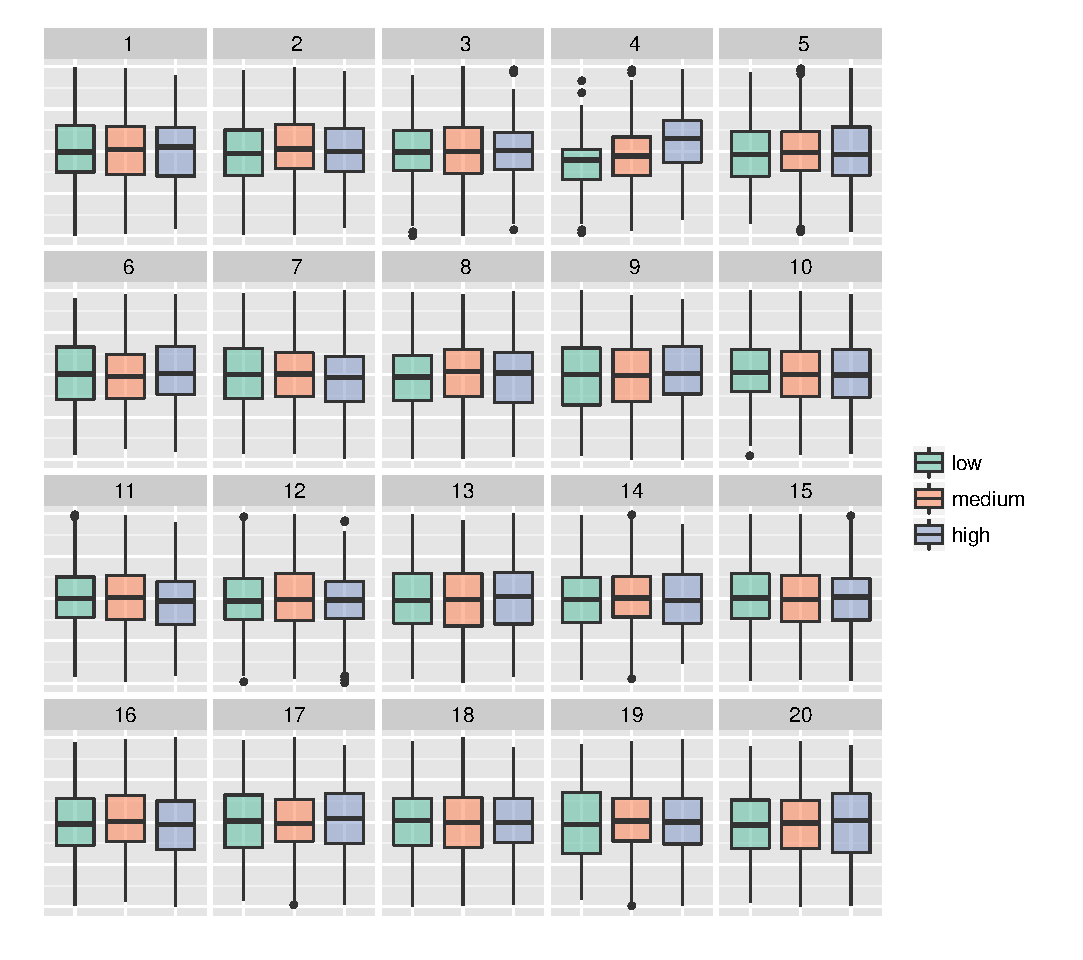
\includegraphics[width=\textwidth]{autism_sicdegp_level1_lineup5.pdf}
%	\caption{\label{fig:boxplot-ordered} Lineup testing for the significance of social skills (low, medium, or high) for a longitudinal model investigating investigating the development of social skills from childhood to adolescence for children diagnosed with autism spectrum disorder. Here the level-1 residuals are used to see if the variable accounts for any additional residual variability. Which is the real plot?}
%\end{figure}
%
%\todo[inline]{I also included the unordered boxplots so we could look at the difference}
%
%\begin{figure}
%	\centering
%	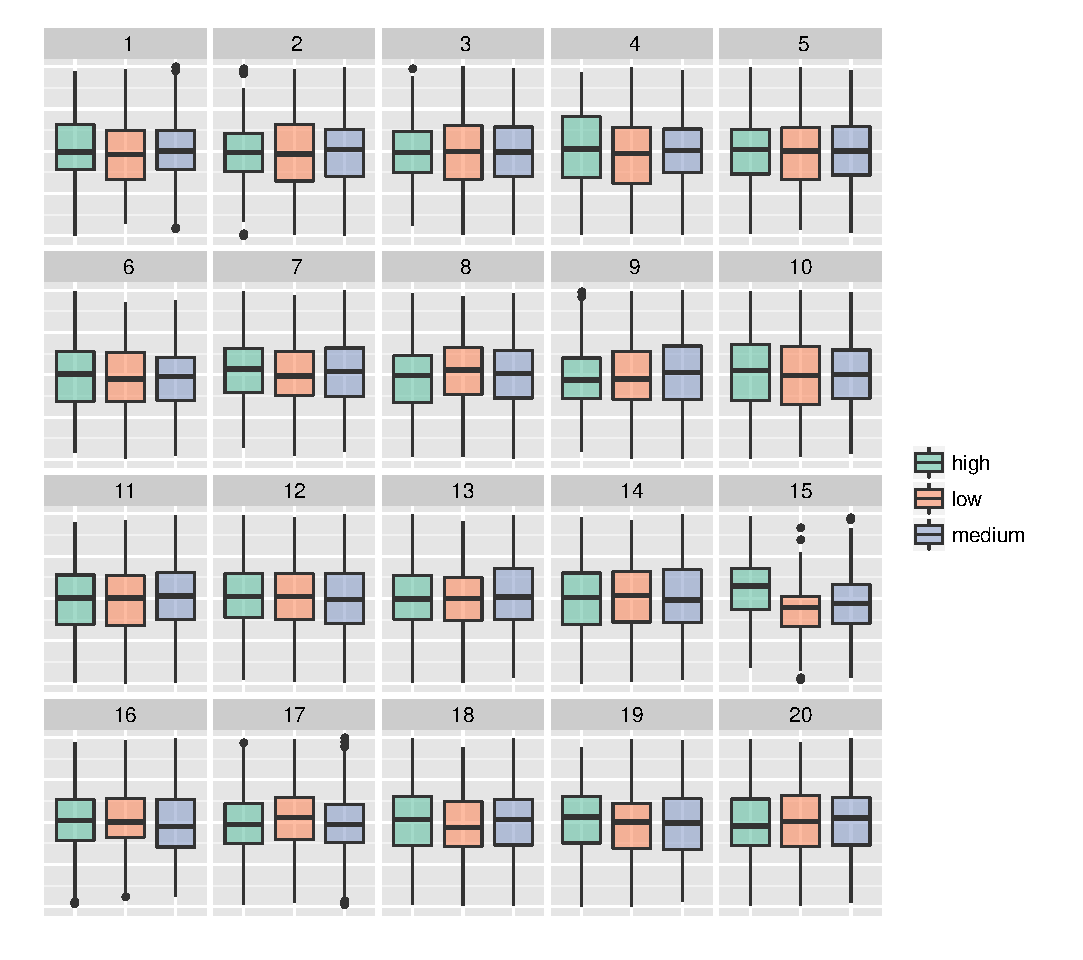
\includegraphics[width=\textwidth]{autism_sicdegp_level1_lineup4.pdf}
%	\caption{\label{fig:boxplot-unordered} Lineup testing for the significance of social skills (low, medium, or high) for a longitudinal model investigating investigating the development of social skills from childhood to adolescence for children diagnosed with autism spectrum disorder. Here the level-1 residuals are used to see if the variable accounts for any additional residual variability. Which is the real plot?}
%\end{figure}

%To illustrate the use of visual tests for fixed effects...\todo{Choose a data set!}


%\paragraph{Random effects.} Tests of the random part of a hierarchical model focus on two questions: (1) whether a marginal random effect improves the model and (2) whether allowing the random effects to be correlated improves the model. Different plots must be used to answer each question. To answer the first question, we suggest plots comparing the response and the explanatory variable of interest using appropriate (often linear) smoothers for each group. Scatterplots comparing the predicted random effects can be used to answer the second question.
%
%\hh{The lineup in figure~\ref{fig:fanned} is chosen to test the relationship between scores from the General Certificate of Secondary Education exam (GCSEE) and the  standardized London Reading Test (LRT).  Each line segment represents one of 65 inner-London schools. The slope of each line is determined by a linear regression of the two test scores for all students at a school. 
%The question of interest is whether random slopes for LRT scores are required to  represent the relationship between GCSEE and LRT scores ($H_1$). Correspondingly, data for the null plots  is  created by simulating GCSE exam scores from a model with a random intercept only.}
%\hh{The resulting scores for each school are regressed on LRT results and shown as lines} 
%%\al{and overlaying linear smoothers for each school.}
%
%
%%
%%Revisiting Figure~\ref{fig:fanned} we see an example of testing for the inclusion of a random effect. Recall that the initial model was a random intercept model using a student's score on the standardized London Reading Test to describe their age 16 score on the General Certificate of Secondary Education examination.
% %To construct this figure we used the parametric bootstrap to generate simulated GCSEE exam scores, fit separate regression models to the simulated responses, and then plotted the fitted model for each school. 
% If the model is appropriate, then the \hh{overall pattern of the lines in the null plots} should resemble the observed data. In this example, we find that the true plot (panel $\sqrt{144} + 1$) is identifiable 
%  \todo[inline]{we don't know that the true panel is identifiable, we do need to wait for the results first.}
%  \todo[inline]{true. I suppose I was just writing with an expected outcome in mind.}
%  as the variance of GCSEE scores is larger for higher scores on the standardized LRT than in the null plots; thus, we find evidence supporting the inclusion of a random slope for standardized LRT. This conclusion agrees with the results of the likelihood ratio test, and did not require the use of an asymptotic distribution to calculate the $p$-value.
%
%Having considered the value of a random slope in the model, we next consider whether the model needs to allow the random slope and intercept to be correlated ($H_1$). While this is an example of a standard likelihood ratio test problem, as a correlation of 0 is not on the boundary of the parameter space, a using a lineup keeps tests of the random effects in a unified framework. The lineup in Figure~\ref{fig:ranef-corr} shows scatterplots of the predicted random effects with a linear smoother. The null plots are created by simulation from the model that does not allow for correlation between the random effects, and the true plot is created using the predicted random effects from a model allowing for correlation between the random effects. If the correlation between the random effects is not necessary, then the true plot will display little correlation and be indistinguishable from the null plots. In Figure~\ref{fig:ranef-corr} the true plot (panel $\sqrt{70 + 11}$) is easily identified, providing evidence supporting the inclusion of the additional parameter.
%
%\begin{figure}
%	\centering
%	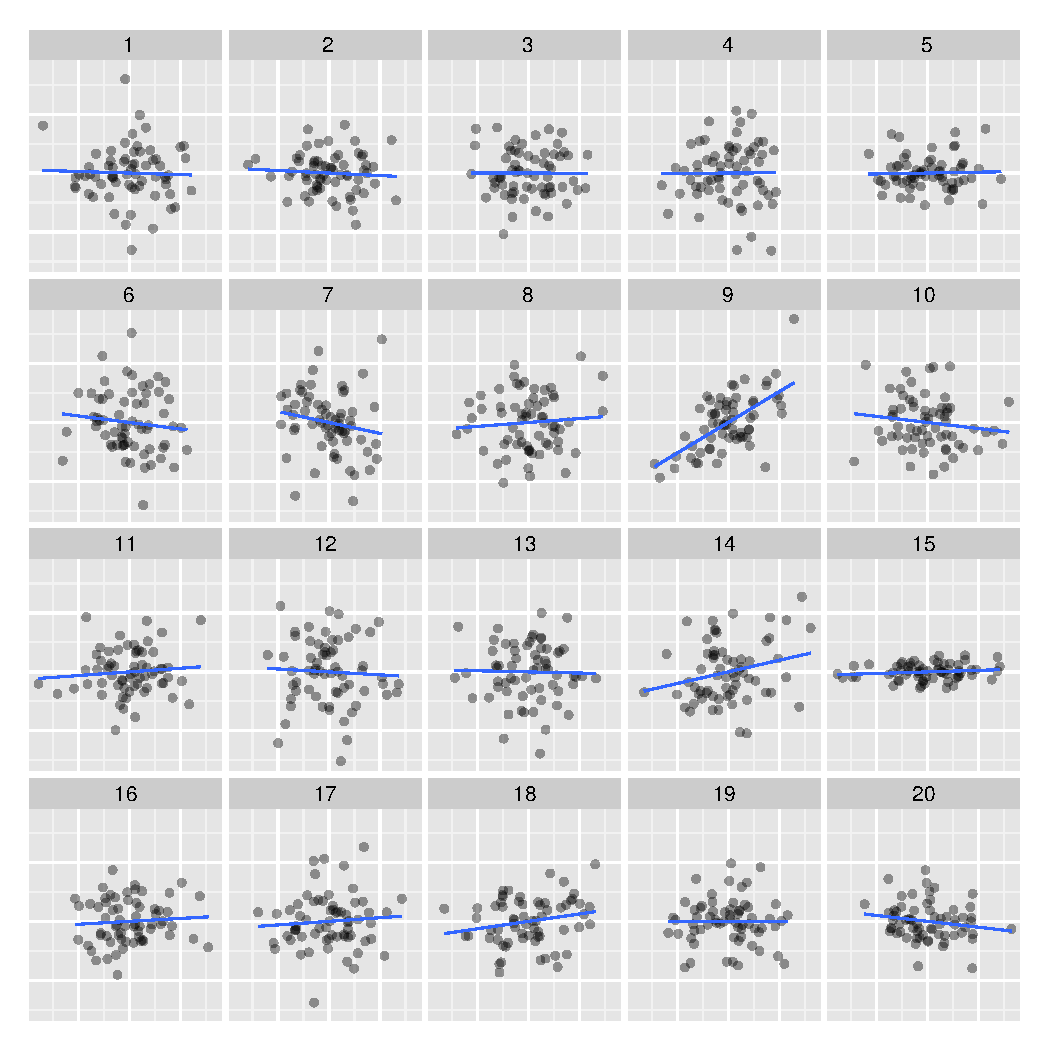
\includegraphics[width=\textwidth]{normexam_corr_lineup9.pdf}
%	\caption{\label{fig:ranef-corr} Lineup testing the need to allow for correlation between the two random effects. These 20 plots compare the predicted random intercept and slope for the model fit to the Exam data. Which is the real plot? Note that this is the type of plot that \cite{Morrell:2000ve} discussed. If there were a higher degree of shrinkage in the random effects we would start to see more false lines in these plots, but as it is, if you remove the smoother and use $\alpha$-blending a line/curve is visible consisting of the random effects of children with only one observation.}
%\end{figure}
%
%\begin{figure}
%	\centering
%	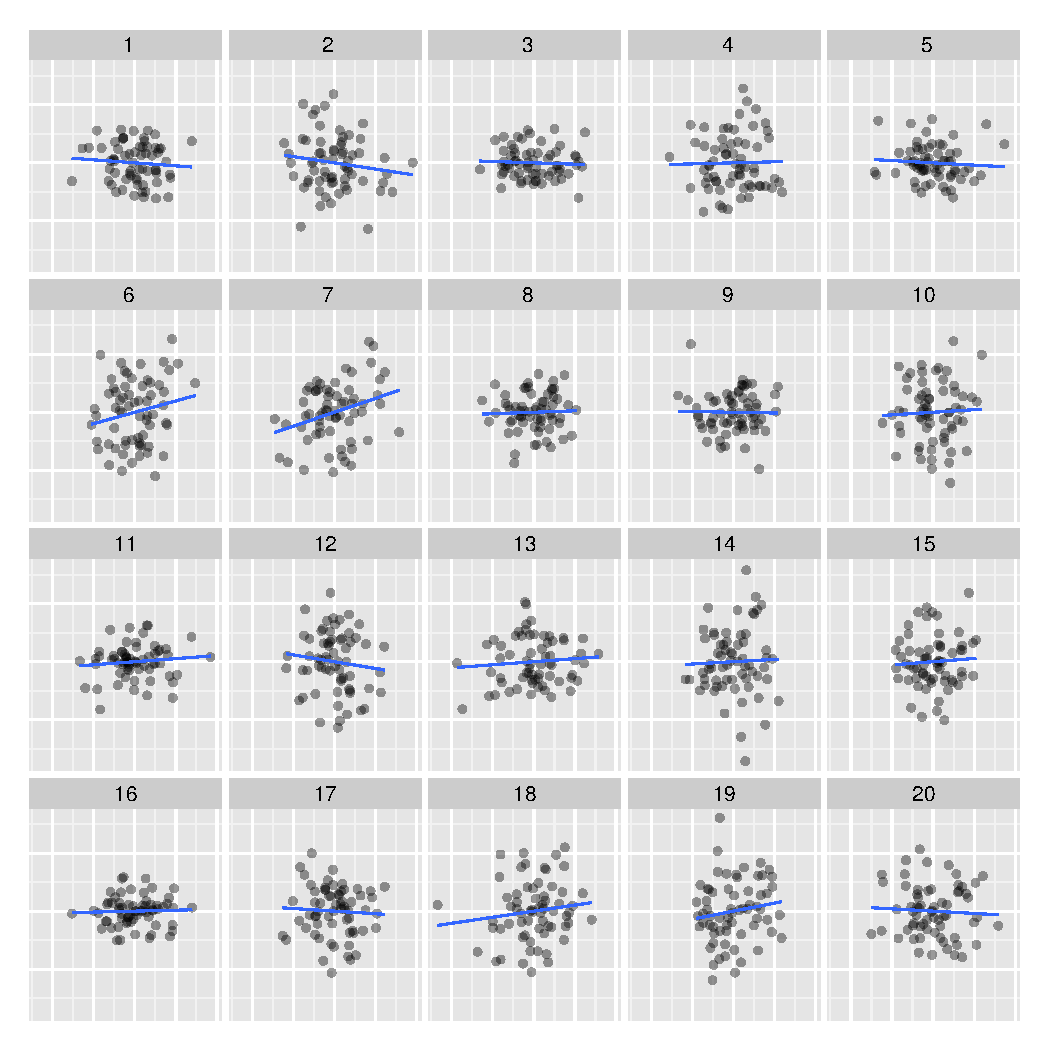
\includegraphics[width=\textwidth]{normexam_uncorr_lineup13.pdf}
%	\caption{\label{fig:ranef-uncorr}  Lineup testing the need to allow for correlation between the two random effects. These 20 plots compare the predicted random intercept and slope for the model fit to the Exam data. Which is the real plot?}
%\end{figure}

%\paragraph{Comparing non-nested models.}
%If two non-nested models are being considered, visual inference can be used to investigate the goodness-of-fit of each model (see Section~\ref{sec:checking} for further discussion). If inadequacies are discovered in one model but not in the other, then this support the use of the properly specified model. This approach is similar in concept to comparing the AIC from each model; however, by focusing on an investigation of how the true data depart from the assumptions made by the model we can see why one may be preferred.


%------------------------------------------------------------------------------------
\section{Model checking}\label{sec:checking}
%------------------------------------------------------------------------------------

In the formulation of model \eqref{eq:hlm} we make a number of assumptions that must be satisfied. In this section we discuss how residual plots can be used with lineups to check the assumptions of homogeneous residual variance, linearity, and normality of the random effects. While we only focus on these assumptions, the discussion is general enough to reveal how visual inference can be extended to check other aspects of the model.

%
%The lineup protocol presents a unified approach to overcome the difficulties encountered when checking the validity of a hierarchical linear model. The only change necessary to utilize this approach to model checking is the generation of null plots, for which we use the parametric bootstrap. Consequently, the ``standard'' residuals plots can be used within this framework in order to overcome the subjectiveness of interpretation and identification of artificial structures, making visual inference a natural extension of conventional model checking. In this section we discuss several examples of lineups that we have found useful for model checking; however, we do not intend to present an exhaustive overview.


\subsection{Homogeneity of variance}\label{sec:homogeneity}
%\subsubsection{Conventional practices}\label{sec:conv-check}
%------------------------------------------------------------------------------------


%\alnote{I know that the turk study for this first lineup was off because of the data thinning we had to do, but do we want to totally scrap this piece? We could use it as an example of the structure we might observe, and then use the other lineup with the study. I am not sure how well that would flow, but I thought it provided a better example of the artificial structure.}

%\hhnote{***LINEUP*** for homogeneity - what about the dialyzer example with side by side boxplots for flow speed}

%\alnote{I included such a lineup, though I am not sure if it quite what we want.}

%\hhnote{I like the boxplots a lot - but in the study, let's include both the boxplots and an example with jittered dots - I would like to check on the power between the designs. I would assume that boxplots are better (we've seen that before in the infovis paper \cite{infovis:2011}), but it would be nice to confirm it. }

%\hhnote{I'm including two more plots here - figures~\ref{homogeneous-1} and \ref{homogeneous-2}. They are both plots of residuals by subject. For the dot plots, I liked the idea of the sorting by group - so here, we sort groups by increasing variance - all the groups are the same size, but the sorting is different for each one. I believe that we cannot pick the data (it's at least difficult), i.e. there is homogeneity, but I like the way that the plot fans out. It might be a bit busy, though. To be fair, the box plots would probably also have to be sorted, but they aren't at the moment.}

%\begin{figure}[hbt]
%	\centering
%	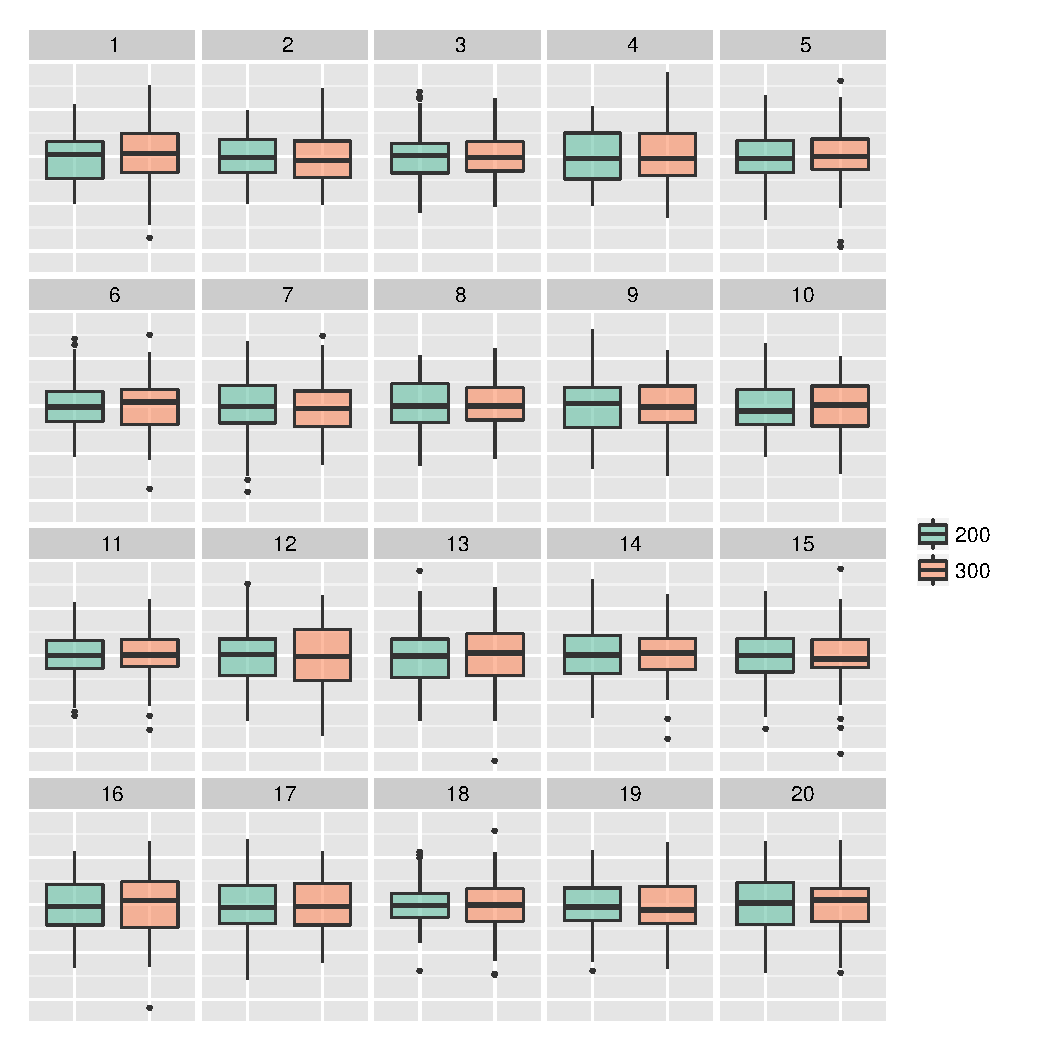
\includegraphics[width=.9\textwidth]{dialyzer-boxplots-lineup15.pdf}
%	\caption{ 
%	Lineup testing homogeneity of the level-1 residuals. Which of the plots is the most different? Which feature led you to your choice?
%%	Lineup of 20 scatterplots of level-1 residuals against pressure used to test the assumption of homogeneous level-1 residual variance for the dialyzer study.  Which is the real plot?
%\hh{We did not test this one, but I would assume that participants identify the true plot because of the outliers in the same way as the box plot of the other lineup}}
%\end{figure}


Model~\eqref{eq:hlm} assumes homogeneity of the within-group variance. To check this assumption we must verify the homogeneity of the within-group residual variance across the levels of all explanatory variables and check that the within-group variance is also constant between groups. Such investigations are often carried out using plots of the level-1 residuals. In order to guard against mis- or over-interpretation of the residual plots, we can again employ lineups.

%For example, consider investigating the appropriateness of this assumption for the GSCEE data. 
%To check the homogeneity of variance across the values of the explanatory variables we utilize plots of the level-1 residuals.
%Such plots are appropriate to check the assumptions of linearity and homoscedasticity at each level of the model. 
%The lineup in 
%Figure~\ref{fig:constvar1} shows a lineup of 20 plots of the level-1 residuals against a cubic fit in standardized LRT scores, one of the explanatory variables included in the model. If any panel of this lineup is considered separately, an analyst may come to the conclusion that the within-group variance decreases as (standardized LRT scores)$^3$ increases; however, inserting the true plot into the lineup forces the analyst to consider the features such a plot will exhibit under the null hypothesis of homogenous variance. Based on the lineup, is there a violation of this model assumption? If we identify the true plot (panel $\sqrt{121} - 8$) this provides evidence of a violation, but if we are unable to, this provides evidence that any structure observed in the plot is artificial.


\begin{figure}[hbt]
	\centering
	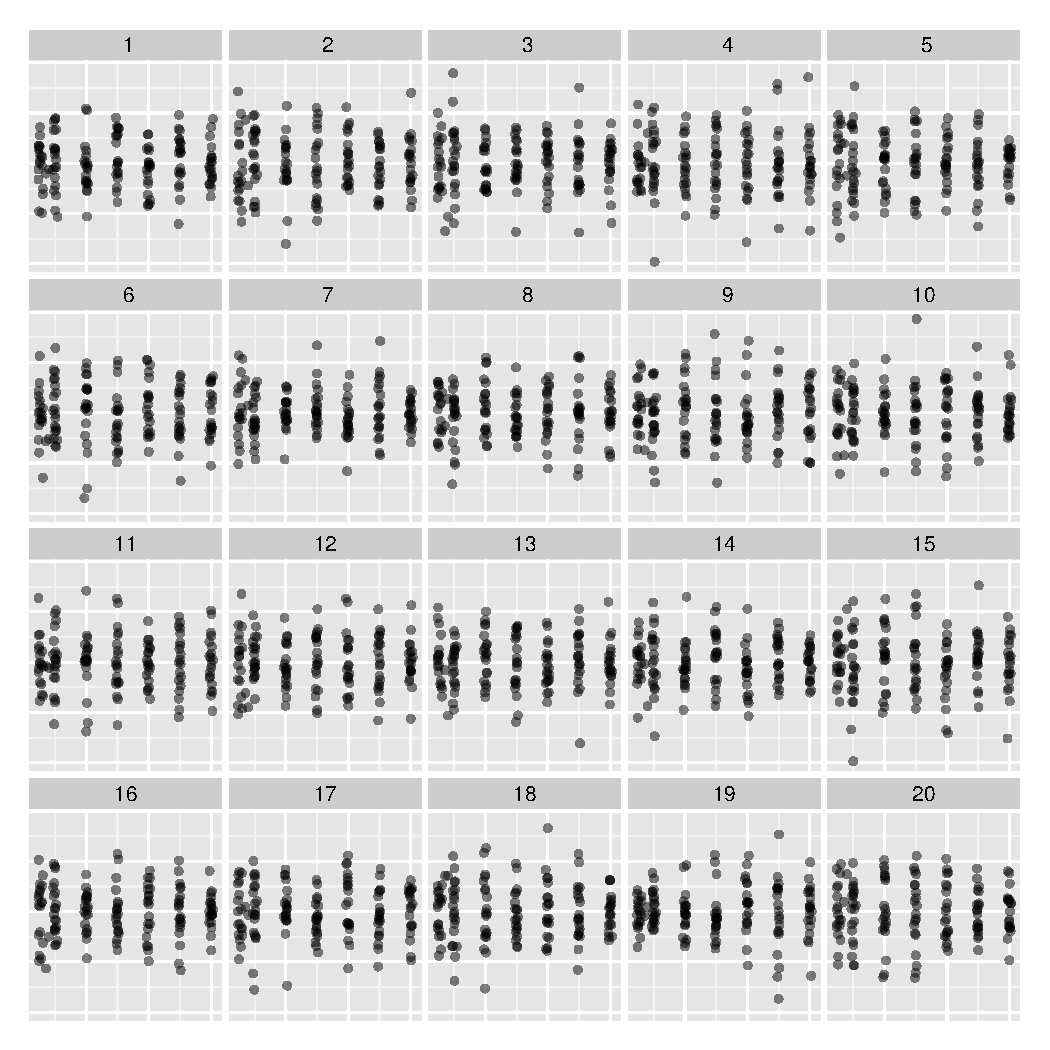
\includegraphics[width=0.8\textwidth]{dialyzerheterogeneous-19.pdf}
	\caption{\label{fig:constvar2} 
	Lineup testing homogeneity of the level-1 residuals. Which of the plots is the most different? Which feature led you to your choice?}
%	Lineup of 20 scatterplots of level-1 residuals against pressure used to test the assumption of homogeneous level-1 residual variance for the dialyzer study.  Which is the real plot?}
\end{figure}



Figure~\ref{fig:constvar2} shows a lineup of 20 plots of the level-1 residuals against pressure in the dialyzer study (see Appendix~\ref{data:dialyzer}).
%If any panel of this lineup is considered separately, an analyst may come to the conclusion that the within-group variance decreases as pressure increases \al{XXX I don't see that anymore XXX}; 
%\hhnote{you're right - this description seems to refer to the wrong lineup ... it should be one of the cyclones or fig~\ref{homogeneous-1}. Should we switch the order of 7 \& 8 and 5 \& 6 ...? }
%however, inserting the true plot into the lineup forces the analyst to consider this particular feature as inherent to the data structure rather than evidence against a hypothesis of homogenous variance. 
 In this example 29 of 85 observers identified the true plot in panel \#($2^4 +3$), providing evidence of heteroscedasticity. 
 %\hhnote{discuss reason that participants gave for their choice.}




%\hh{An example for the use of a lineup where observers do not detect heteroscedasticity and an accompanying discussion can be found in appendix~\ref{app:morelineups}.}
%\hhnote{where should the next sentence go? also in the appendix? - it's making a nice point, though}
%Comparing the two lineups reveals that the patterns that can be expected in any given residual plot differ depending on the data set. The use of lineups incorporates the comparison of the data to what is expected, eliminating the subjective interpretations we encounter with the use of single plots. 
%\alnote{Move the last sentence above into cyclone plot discussion -- any individual panel may lead someone to suspect structure where there is none.}


%\begin{figure}
%	\centering
%:
%	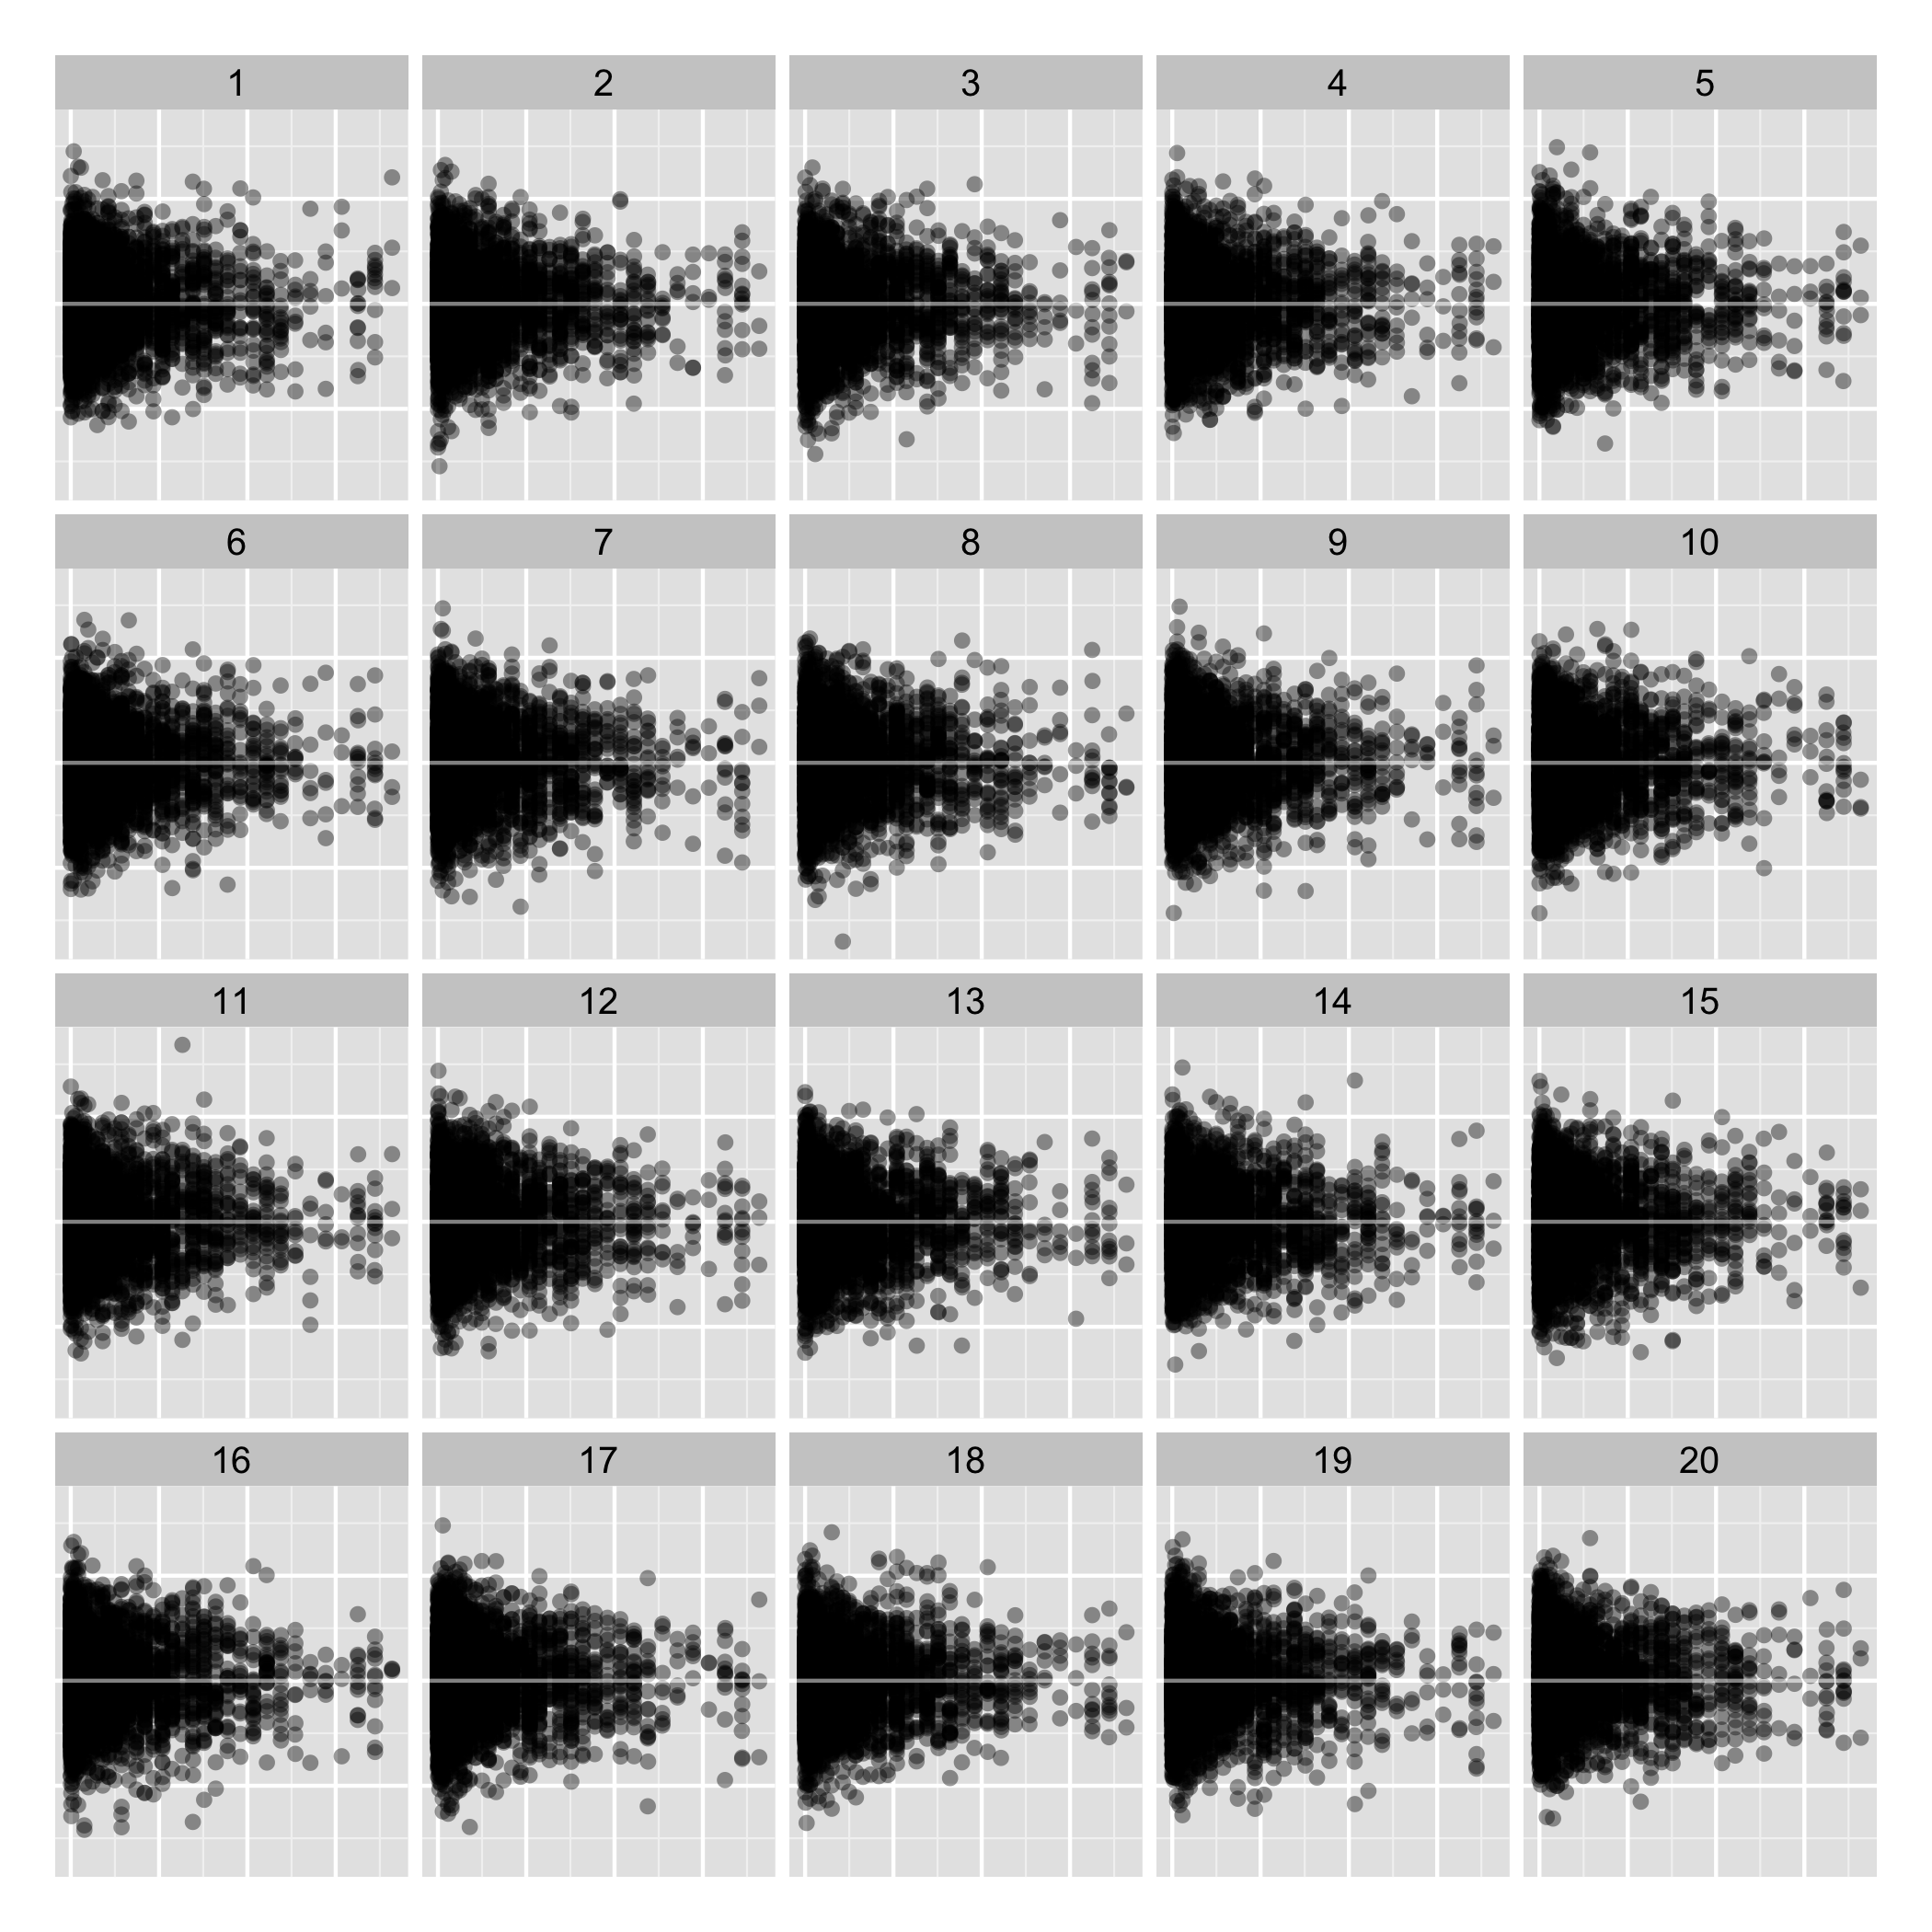
\includegraphics[width=\textwidth]{normexam_constvar_lineup3.png}
%	\caption{\label{fig:constvar1} 
%	Lineup testing homogeneity of the level-1 residuals. Which of the plots is the most different? Which feature led you to your choice?\hh{We need to figure out what to do with this example. }}
%%	Lineup of 20 scatterplots of level-1 residuals against (standardized LRT)$^3$ used to test the assumption of homogeneous level-1 residual variance.  Which is the real plot?}
%\end{figure}

%\hhnote{I am not quite sure about the difference between cyclone plots and the last four lineups ... We should comment on that.}

%\paragraph{Testing homoscedasticity across groups.}
Residual scatterplots are useful in checking that level-1 residuals are homoscedastic with respect to the explanatory variables, but they do not show the same power as box plots when they investigate potential differences in variability between groups, as can be seen in the example of the lineups in Figures~\ref{homogeneous-1} and~\ref{homogeneous-2} of  Appendix~\ref{app:morelineups}. 
%\alnote{Rethinking this, scatterplots can be used for this (figure 6 shows this!), but there are more effective plots.}
To visualize this assumption, we suggest using side-by-side box plots of the level-1 residuals. 
While box plots are more powerful, they still require the use of lineups.
When the plots are considered individually, unbalanced group sizes will cause artificial structure in these plots. 
%This is to be expected as the variance of the sampling distribution of the level-1 residuals within each group, $\var \left( s_i^2 \right) = \left(2 \left( \sigma_i^2 \right)^2 \right) \big/ (n_i - r_i)$, where $r_i = \mathrm{rank}(\bm{X}_i)$, depends on the group size, $n_i$.
To overcome this difficulty, we create a lineup of side-by-side box plots for each group ordered by their interquartile range (IQR), which we have come to call a ``cyclone'' plot. Figure~\ref{fig:badcyclone} shows a lineup of cyclone plots for 66 patients in a longitudinal study investigating the ability of methylprednisolone to treat patients with severe alcoholic hepatitis (see Section~\ref{data:ahd} for details). The true plot in panel \#($2^3+5$) is easily identified from the field of null plots (by 50 of 75 observers) revealing heteroscedasticity across groups that might not be apparent  in other residual plots.

While the data plot is \al{easily identified}, any panel from this lineup considered separately exhibits a structure that might, taken by itself, lead an analyst to the conclusion that within-group variance increases across the vertical axis. However, \al{placing} the true plot into the lineup forces the analyst to consider most of this structure as inherent to the data rather than evidence against the hypothesis of homogeneity. The fact that observers are able to still identify the data plot, indicates that the data plot has additional structure inconsistent with homogeneity. The use of lineups incorporates the comparison of the data to what is expected, eliminating the subjective interpretations we encounter with the use of single plots. 

\hhnote{how about the above change? we've got the additional complication that overall the test is significant, while individually each lineup panel shows very similar structure that -surprisingly- is not yet indicative of non-homogeneity.}
\alnote{I like the change! I commented out the original comment/paragraph.}

%\alnote{Smooth this discussion out:}
%
%\al{If any panel of this lineup is considered separately, an analyst may come to the conclusion that the within-group variance increases across the $x$ axis.  However, inserting the true plot into the lineup forces the analyst to consider this particular feature as inherent to the data structure rather than evidence against a hypothesis of homogenous variance.
%
%
%The use of lineups incorporates the comparison of the data to what is expected, eliminating the subjective interpretations we encounter with the use of single plots. 
%}

\begin{figure}[hbt]
	\centering
	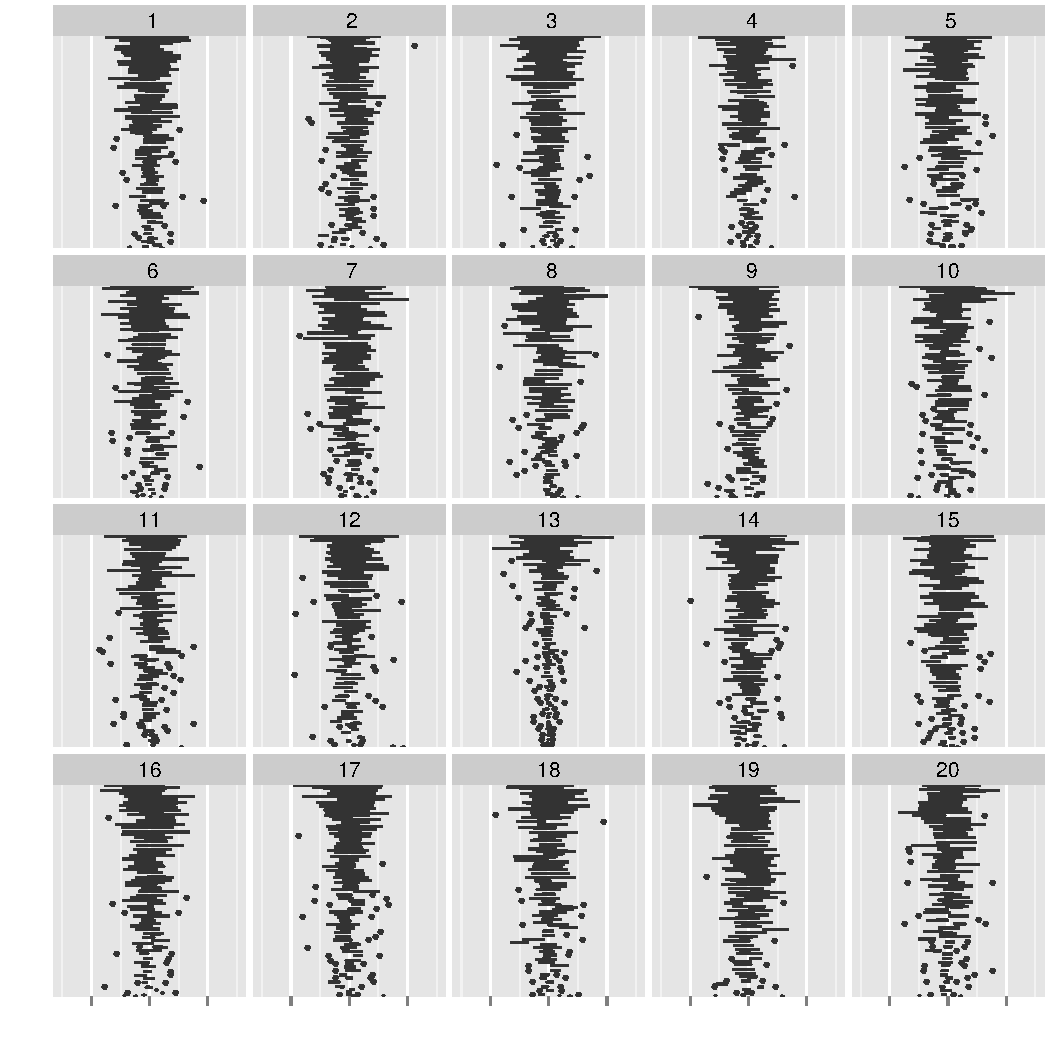
\includegraphics[width=0.8\textwidth]{cyclone-13.pdf}
	\caption{\label{fig:badcyclone} 
	Lineup testing homogeneity of the level-1 residuals between groups. Which of the plots is the most different? Which feature led you to your choice?}
%	Lineup of 20 boxplots (ordered by IQR) of level-1 residuals used to test the assumption of homogeneous level-1 residual variance.  Which is the real plot?}
\end{figure}

An alternative approach to detect homoscedasticity of the level-1 residuals across groups is to use a test based on the standardized measure of dispersion given by
%
\begin{equation}\label{eq:d}
	d_i = \frac{\log\left( s_i^2 \right) - \left[ \sum_i (n_i - r_i) \log\left( s_i^2 \right) / \sum_i  (n_i - r_i) \right]}{\left(2 / (n_i - r_i)\right)^{1/2}}
\end{equation}
%
where $s_i^2$ is the residual variance within each group based on separate ordinary least squares regressions and $r_i$ is the rank of the corresponding model matrix  \citep{Raudenbush:2002}. The test statistic is then
%
\begin{equation}
	H = \sum_{i=1}^{g^*} d_i^2
\end{equation}
%
which has an approximate $\chi^2_{g^*-1}$ reference distribution when the data are normal and the group sizes are ``large enough''. Here we use $g^*$ because ``small'' groups may be excluded from the calculation as small group sizes provide less reliable information about the residual variance, but this is a subjective choice. A common rule of thumb is to exclude groups with samples sizes smaller than 10. If the distributional assumptions are violated, or we do not have large enough group sizes,  the approximation to the $\chi^2$ distribution breaks down. In the methylprednisolone study each subject was observed at most five times, with 19 subjects dropping out of the study early. Due to the small group sizes the $\chi^2$ approximation is inappropriate, forcing the analyst to rely on simulation to construct the sampling distribution of the test statistic, which is not only computationally more demanding than the generation of 19 null plots, but lacks power with small sample sizes. Performing the simulation-based version of the test in this example results in a $p$-value of 0.0886, providing much weaker evidence for heterogeneity than the visual test. 

%\alnote{I need to go back and really emphasize the lack of effective conventional tests here}
%\hhnote{what is the result - in $p$-value for the conventional test? it would be nice if it were inconclusive :) }
%\alnote{Unfortunately, the result was not inconclusive ($p$-value $<$ 1e-4), however, the test statistic is based on LS regression using only 4 or 5 observations for each model. This seems dubious!}
%
%\hhnote{and we need a second cyclone plot (that probably ends up in the supplementary material, but still ... ***LINEUP***  to show a situation with different group sizes, i.e. the cyclone structure, but non significant variability.}
%\alnote{Here is a cyclone plot made from a reduced set of the radon data. I used the EB residuals here, so not everything is centered around 0, but we could use the LS residuals to overcome that.}
%\hhnote{The centered residuals might work better - or we need to sort differently. Lineups with LS residuals in cyclone plots are added to the study}

\begin{figure}[hbt]
	\centering
	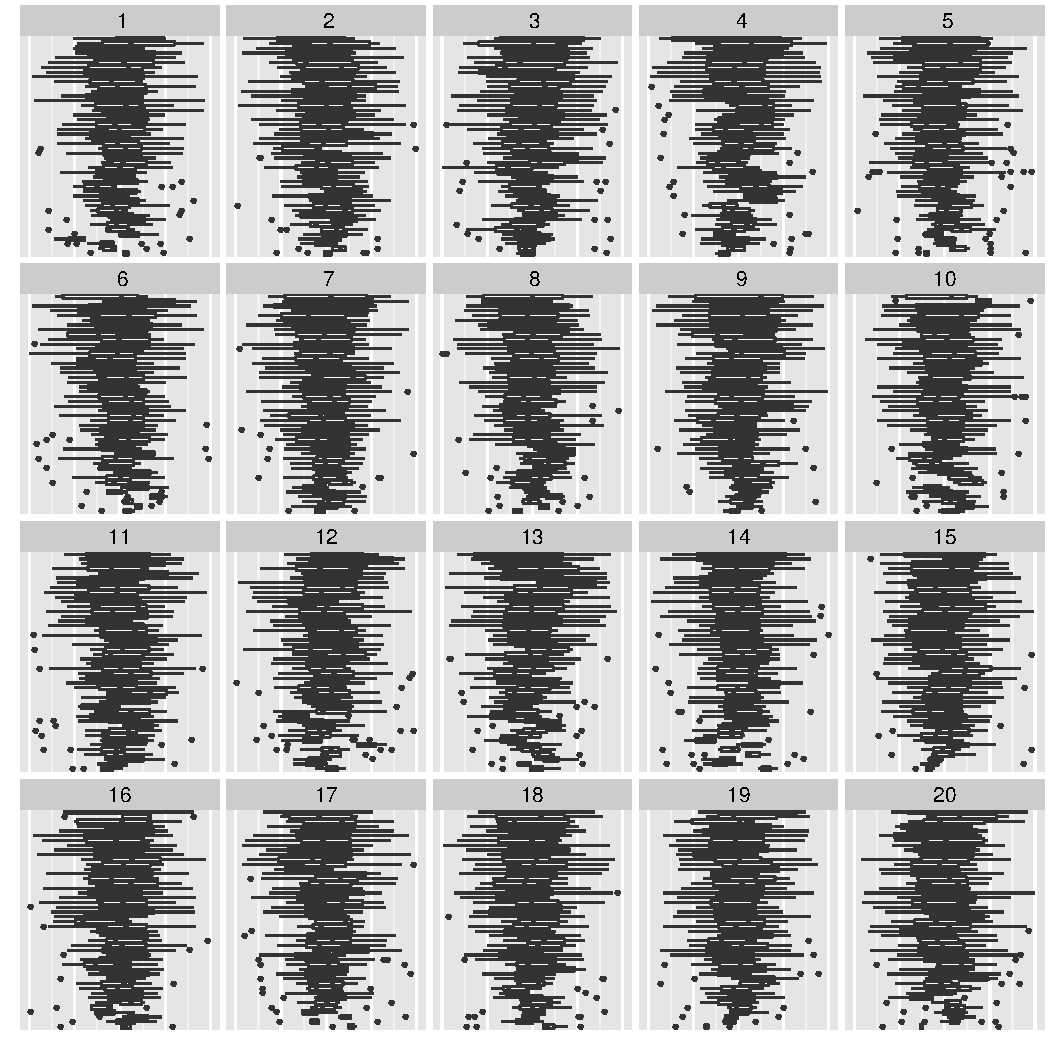
\includegraphics[width=0.8\textwidth]{radon_cyclone10.pdf}
	\caption{\label{fig:goodcyclone} Lineup of 20 box plots (ordered by IQR) of level-1 residuals used to test the assumption of homogeneous level-1 residual variance.  Which is the real plot?}
\end{figure}

\alnote{Construct table of $p$-values for the conventional test with varying group size restrictions.}

%\alnote{Intro data and reference appendix. }
Figure~\ref{fig:goodcyclone} shows another lineup of cyclone plots.  The data underlying this example are radon measurements across counties in Minnesota (see Section~\ref{data:radon} for details).
Here, level-1 residuals by county are plotted from a model, in which only counties with at least five observations were included. 
%Similar \hh{XXX??? -need the $p$-value first! XXX} to the above $p$-value, homogeneity is not rejected based on this lineup.  
Only one out of  59 participants identified the data plot shown in panel \#$(4^2 - 6)$ from the lineup, providing no evidence against homogeneity. In this situation the conventional test yields a $p$-value of 0.149, if counties with fewer than 10 observations are excluded, thereby agreeing with the visual inference result. However, if only counties with fewer than 5 observations are excluded, the conventional test indicates strong evidence of heterogeneity based on a $p$-value of 0.0185. This sensitivity to the group size is a clear weakness of the conventional test, and casts doubt on its usefulness in situations with small group sizes. In contrast, the visual test is not overly sensitive to group sizes. Counties with less than 5 observations were eliminated because box plots are not appropriate for such small group sizes, but could be included in the representation as dot plots. While we are still slightly constrained with group sizes, we are far less constrained than with the conventional test.
 
%\alnote{The ``conventional'' test yields a p-value of about 0.149 (if you use the $\ge 10$ suggestion, it yields a p-value of about .0017 if you use $\ge 5$. For the conventional test, the rule of thumb seems safer, though means we can apply the method only in situations with group sizes of $10+$, which we can emphasize!}

%\begin{figure}
%	\centering
%	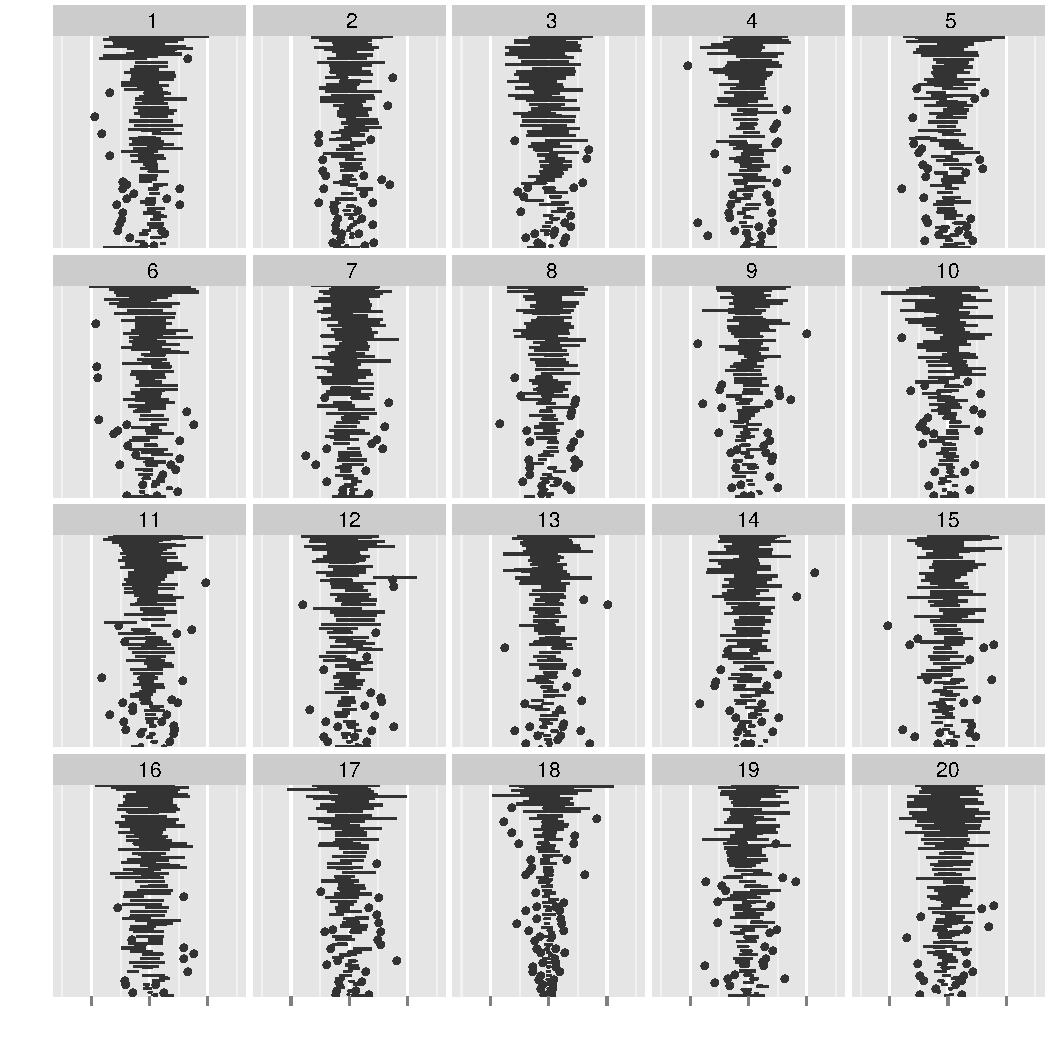
\includegraphics[width=\textwidth]{ahd_badcyclone5.pdf}
%	\caption{\label{fig:badcyclone} Lineup of 20 boxplots (ordered by IQR) of level-1 residuals used to test the assumption of homogeneous level-1 residual variance.  Which is the real plot?}
%\end{figure}

%\begin{figure}
%	\centering
%	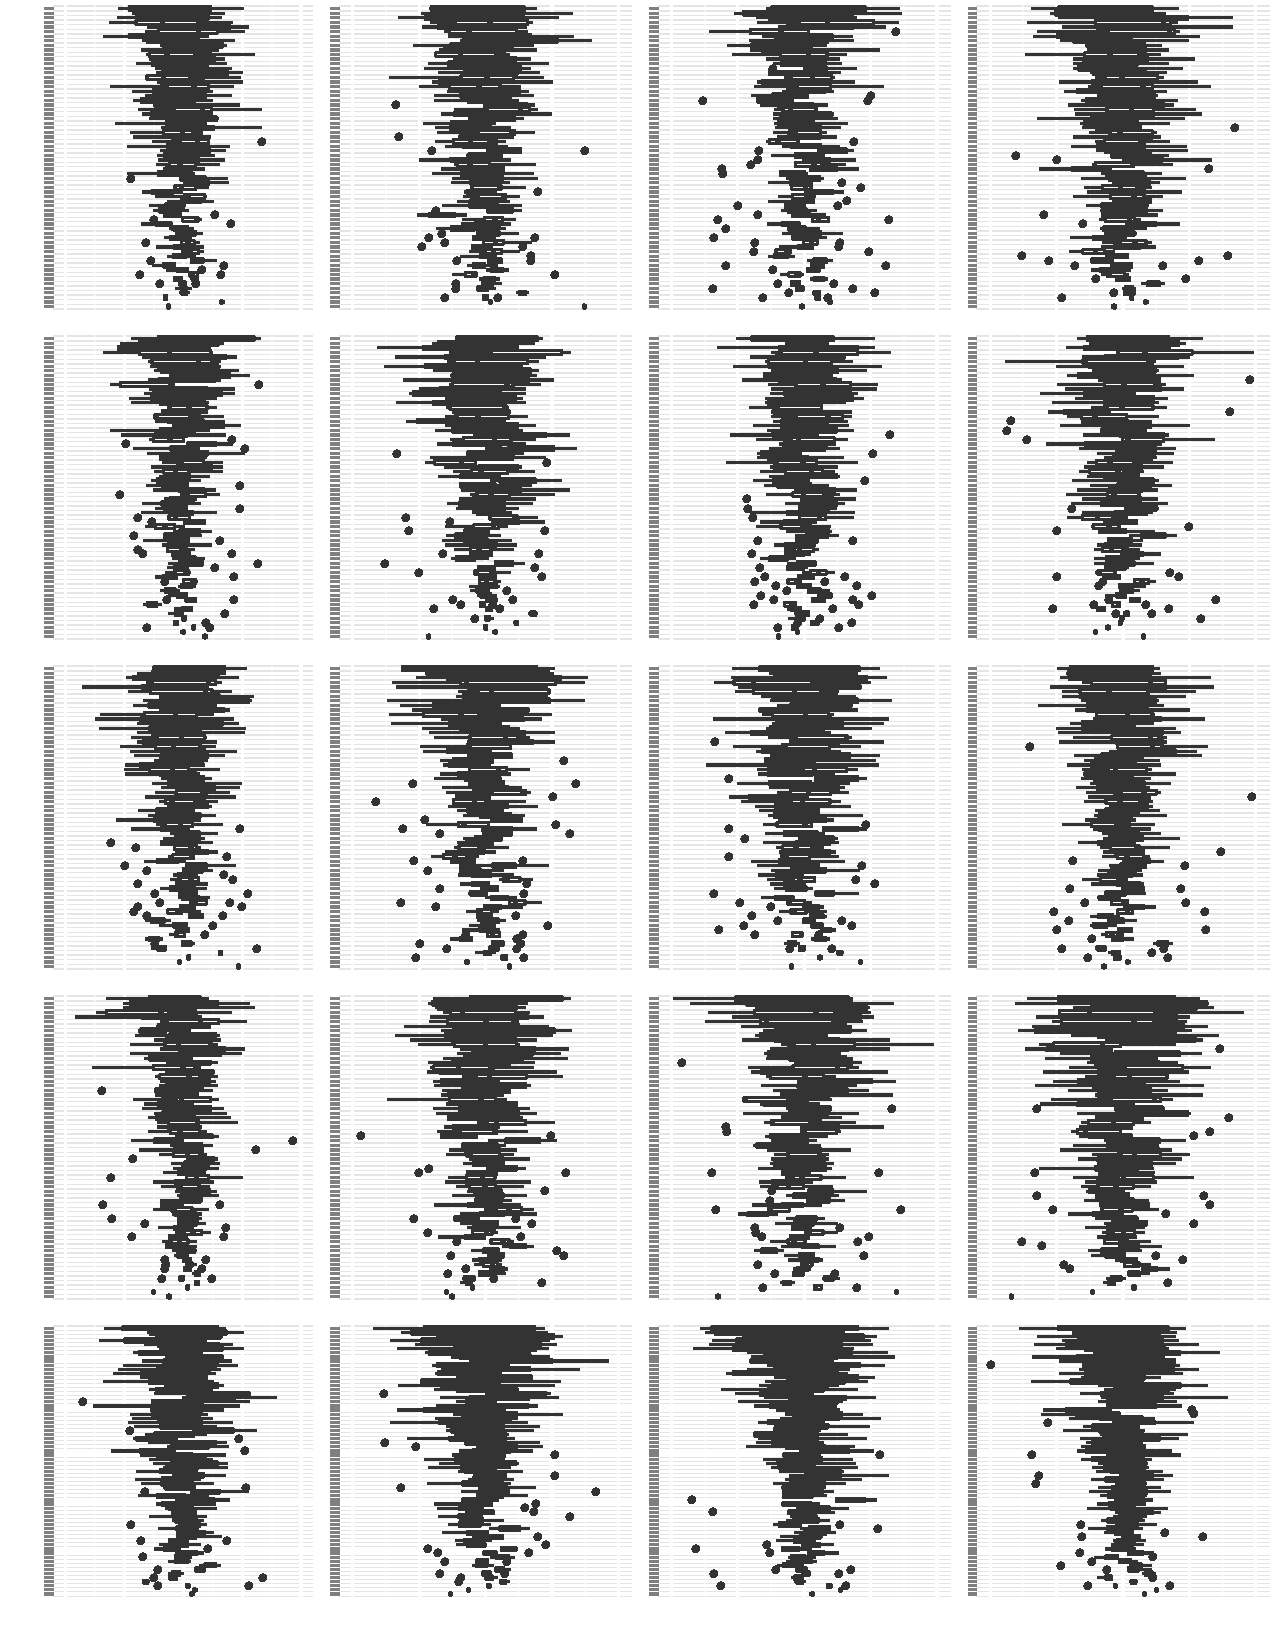
\includegraphics[width=\textwidth]{ahd_goodcyclone13.pdf}
%	\caption{\label{fig:goodcyclone} Lineup of 20 boxplots (ordered by IQR) of level-1 residuals used to test the assumption of homogeneous level-1 residual variance.  Which is the real plot?}
%\end{figure}


\subsection{Linearity}
%------------------------------------------------------------------------------------

Scatterplots with smoothers can also be used to check that the relationship between the explanatory variables and response variable is in fact linear. Figure~\ref{fig:linearity} shows such a lineup testing the linearity of an observation-level explanatory variable. Out of 63 observers, 60 identified the true plot in panel \#($2^3 + 2$), providing evidence that the mean structure is misspecified. This example comes from the dialyzer study and considers a model with only linear and quadratic terms for transmembrane pressure (see Appendix~\ref{data:dialyzer} for details on the data). It is clear that a higher-order polynomial is required. 
%\hhnote{we should probably include a higher order polynomial and come up with a new lineup in which the mean structure is captured correctly (or at least better).}
%\alnote{This is actually what we do in Figure 4, but after the issue with the mean structure is resolved the issue of heteroscedasticity rears its head.}
%\hhnote{Oh, ok - we should still write up a sentence on this}
Once a polynomial of degree four is included in the mean structure of the fixed effects, \al{the nonlinear pattern in} the residuals is \al{removed}---a lineup of this situation is shown in Figure~\ref{fig:constvar2}. In this lineup, the data plot is identified due to heteroscedasticity in the residuals.  This highlights the flexibility of lineups due to the general phrasing of the alternative hypothesis. By tracking observers' reasons for the choice of plot in a lineup, we can distinguish between different alternatives. 
%\alnote{Would ``a unified framework'' be more accurate? I am still milling this over.}
Using the same setup we will get test results based on where we are in the modeling process: as long as the mean structure is not correctly specified, it is most likely the distinguishing feature. Once the mean structure is properly specified, the lineup changes to test for homogeneity of variance. 

\begin{figure}
	\centering
	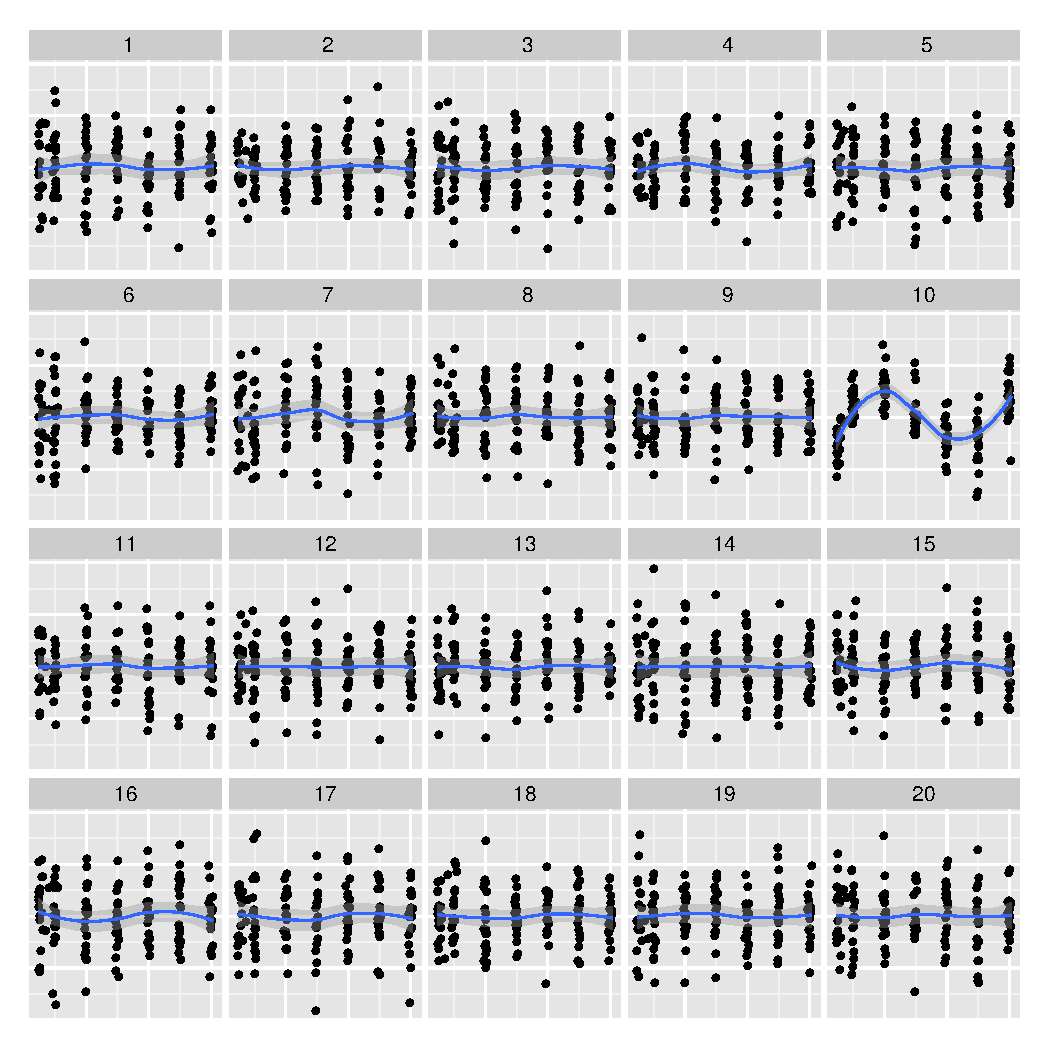
\includegraphics[width=0.8\textwidth]{dialyzernonlinear-10.pdf}
	\caption{\label{fig:linearity} Lineup testing  for nonlinearity of a covariate. Which of the plots is the most different? Which feature led you to your choice?}
%To check the assumption of linearity we suggest the use of scatterplots with smoothers and boxplots of both the residuals (either level-1 or -2) against the fitted values of an explanatory variable. If the assumption of linearity is upheld, then the residuals plots will exhibit ``random scatter.'' 
%%As illustrated in the previous section, such plots are also useful in checking for homogeneity of variance, but in that situation different deviations from random scatter are of interest.
%\alnote{I will write more here.}

	%Lineup of 20 scatterplots of level-1 residuals against pressure with a LOESS smoother used to test the assumption of linearity for the dialyzer study.  Which is the real plot?}
\end{figure}

To extend checks of linearity to group-level variables we suggest the use of the level-2 residuals. 
%Additionally, when categorical predictors are investigated, side-by-side boxplots should be used.
%\alnote{If we're looking for anything to cut, the last sentence is a prime target.}

%\hhnote{we wanted to talk about how this is the most familiar situation and is entirely solvable with tools straight from linear models. Did Cook and Weisberg name those? I think I've seen the name partial residual plots at times. 
%We need another ***LINEUP*** here, we agreed to use a quartic term in the dialyzer example to have a better mean structure.}
%\alnote{See the above note for a comment on the mean structure.\\[1em] 
%
%
%I am not sure if Cook and Weisberg named the scatterplots with smoothers, but they are not quite partial residual plots. Partial residual plots use the augmented (larger) model to construct residuals using fixed effects estimates for a reduced set of variables. Added variable plots are also similar in spirit to partial residual plots, though they are more involved. Partial residual plots have been discussed for mixed models (Hilden-Minton (1995); Hodges (1998)), but what we are doing is simpler in my mind. It might be interesting to pull this parallel into the paper, and maybe even compare what we see in an added variable plot and in the lineup. An extra perk of the lineup here is that added variable plots for LME models are not implement in R, but lineups are easy to create.\\[1em]
%
%Reference to Hodges (1998): Hodges, J. (1998). Some algebra and geometry for hierarchical models, applied to diagnostics. \emph{Journal of the Royal Statistical Society. Series B (Statistical Methodology)}, 60(3), 497--536.\\[1em]
%
%Based on the examples I have seen, visual inference seems to overcome the problems of interpreting slopes observed on residual plots that was pointed out by Atkinson (1985, p. 67), though I have not formally tested this in any way. Perhaps it would be interesting to do that? Of course, this is most straightforward in the OLS regression setting. 
%}
%\hhnote{this is where we want to extend the discussion a bit: the partial residual plots and our approach is like the difference between type I and type III sums of squares - i.e. looking at the contribution of covariates either without regarding any of the covariates (type III) or only after adjusting for everything else, in which case we need to fit the model first before we can look into the relationship between $Y$ and $X_i$}


\subsection{Normality}
%\hh{This section consists of two parts: we first discuss how to assess distributional assumptions in linear mixed-effects models, which are complicated by confounding issues between levels of residual structures; in the second part we assess power of visual normality tests based on three different Q-Q plot designs.}
%------------------------------------------------------------------------------------

%\subsubsection{Assessing normality of the random effects}
%------------------------------------------------------------------------------------

%Quantile-Quantile (Q-Q) plots \citep{Wilk:1968} are often used as an informal check of the distributional assumptions made on the level-1 and -2 residuals; however, an interrelationship between the residual quantities exists in hierarchical linear models that can render such an assessment inappropriate. 

Recall that in model~\eqref{eq:hlm} we assume that the random effects, $\bm{b}_i$, are a random sample from $\mathcal{N}(\bm{0},\ \bm{D})$ and are independent from the error terms, $\bm{\varepsilon}_i$, which are assumed to be a random sample from $\mathcal{N}(\bm{0},\ \sigma^2 \bm{I}_{n_i})$. In many situations, however, the predicted random effects are highly influenced (i.e., confounded) by the error terms. Consequently, traditional checks for normality such as Q-Q plots and the Anderson-Darling test are not appropriate. 
Formally this is seen by the
strong assumptions that are required for the empirical distributions of the residuals in the linear mixed-effects model to converge in probability to their true distributions \citep[Theorem 3.2 and Lemma 3.1]{Jiang:1998vt}. If these assumptions are not satisfied, then the empirical distribution of the residuals may not resemble the hypothesized distribution under a properly specified model. When this occurs, individual Q-Q plots will often lead to erroneous conclusions about the distributional assumptions which can be overcome, at least partially, using lineups.

Figures~\ref{fig:qqlineup-1} and \ref{fig:qqlineup-t} illustrate the use of lineups to test the distributional assumptions in a linear mixed-effects model. Figure~\ref{fig:qqlineup-1} presents a lineup of the predicted random slopes from the radon study, in which group sizes are very unbalanced and there is a high degree of shrinkage.
\begin{figure}[hbt]
	\centering
%	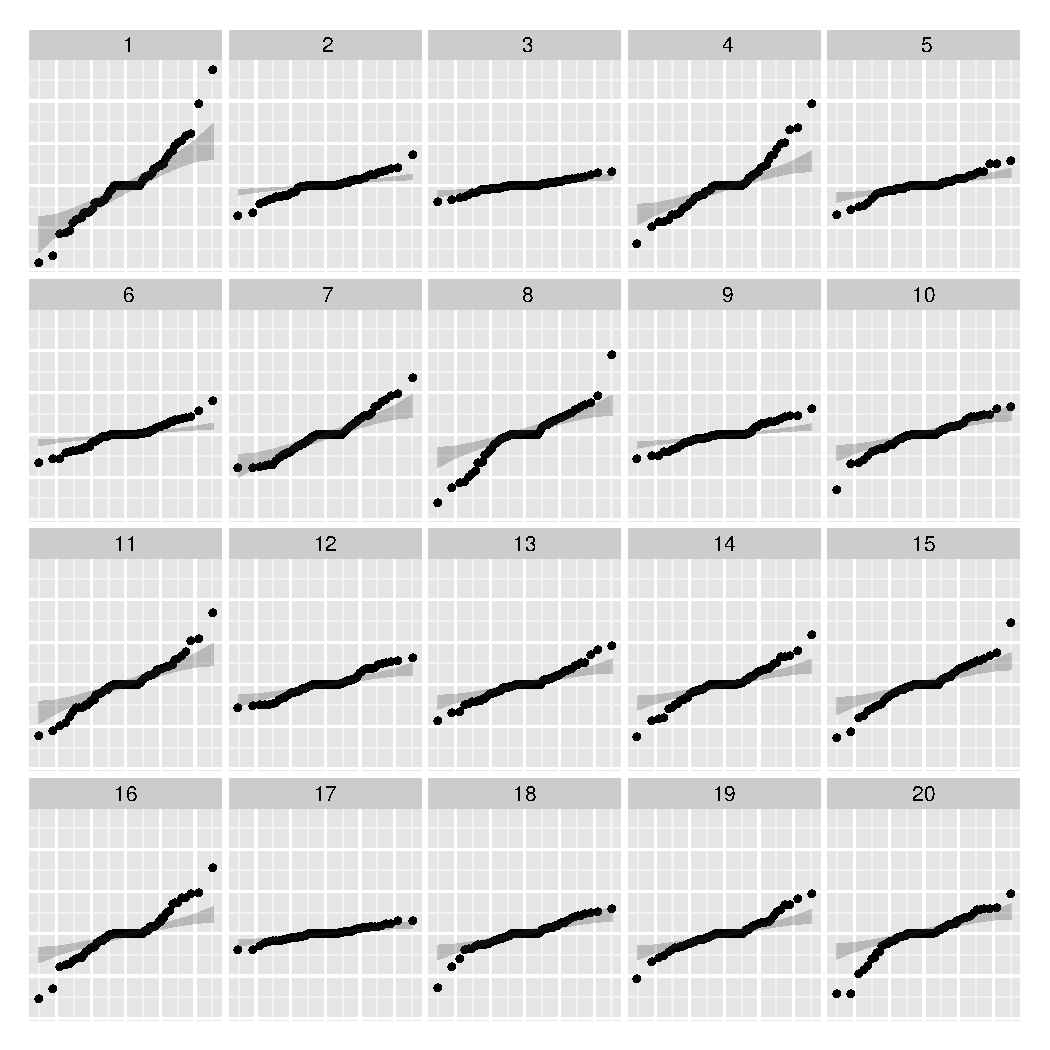
\includegraphics[width=\textwidth]{qqplot_normranef_slope_lineup11.pdf}
%	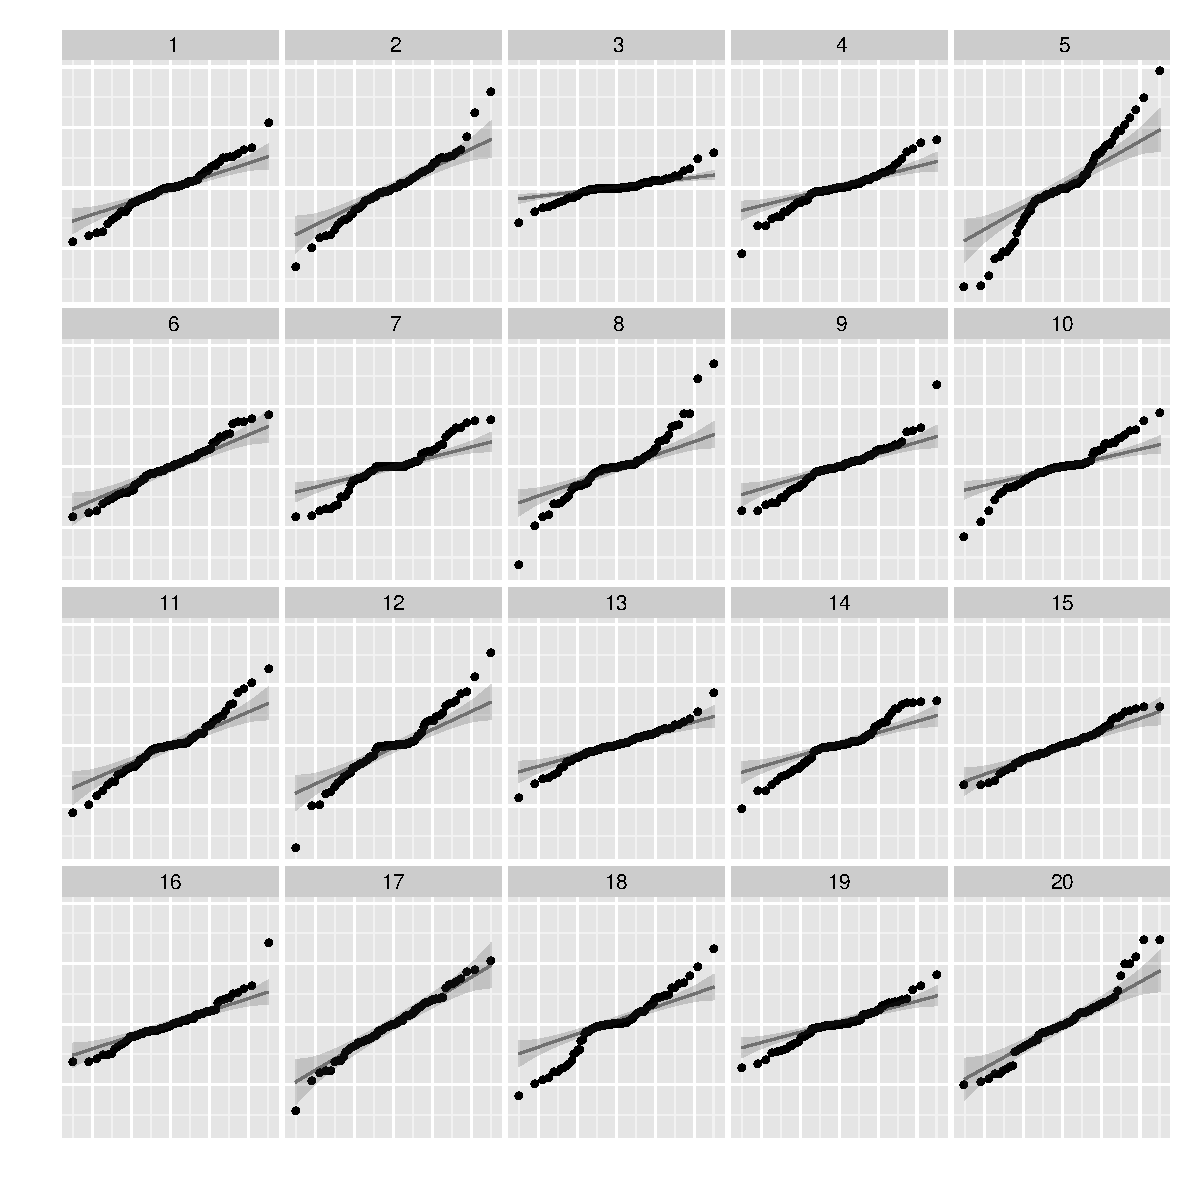
\includegraphics[width=0.8\textwidth]{filebab6182c2e84}
	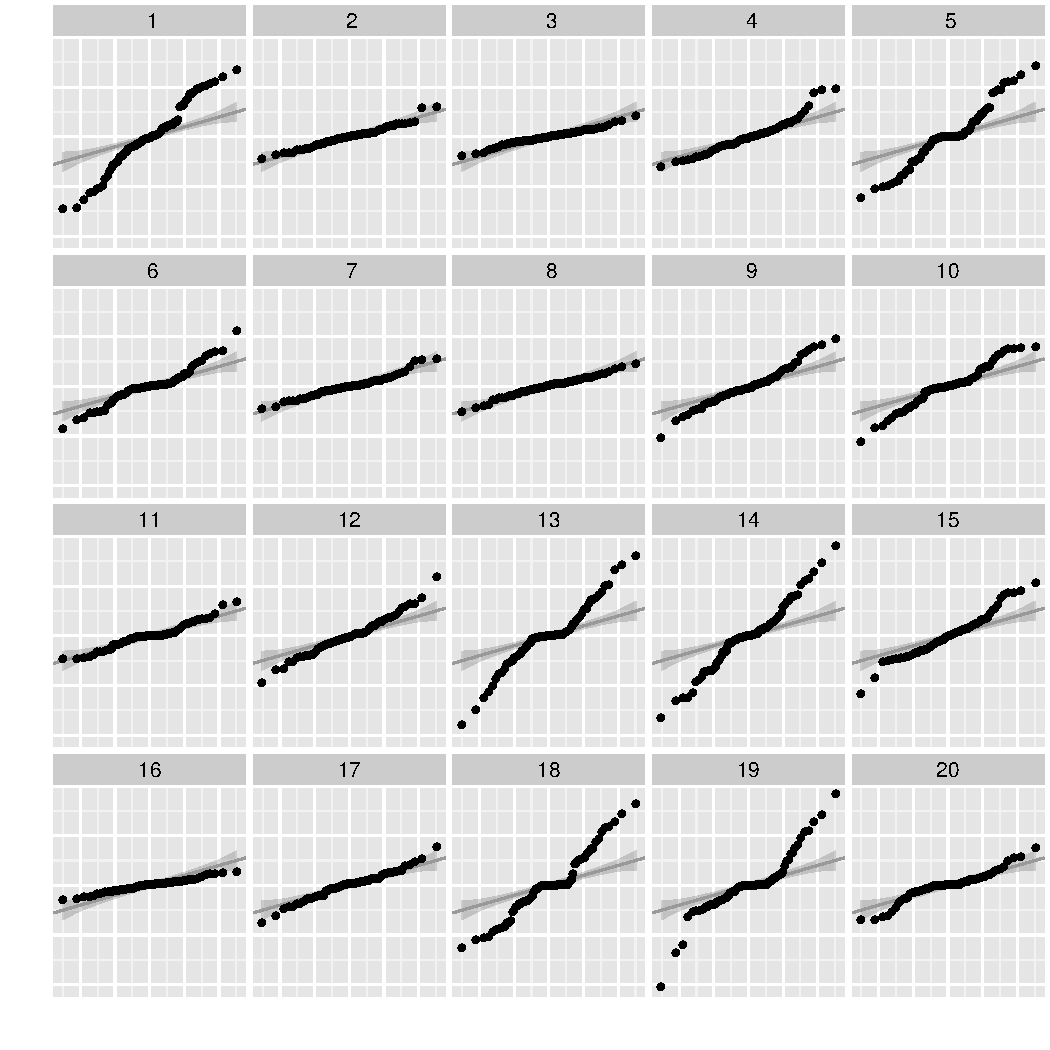
\includegraphics[width=0.8\textwidth]{radonqqb2-3-10.pdf}
	\caption{\label{fig:qqlineup-1}
	Lineup testing  for normality of the random slope for the radon data. Which of the plots is the most different? Which feature led you to your choice? }
\end{figure}

%Both lineups present simulated Q-Q plots of predicted random effects following the design of the radon study (see Section~\ref{data:radon} for details), in which group sizes are very unbalanced and there is a high degree of shrinkage. 
Confidence bands based on the normal distribution were applied to each lineup and reveal that the empirical distribution of the predicted random effects---both for the null plots and true plot---does not align with a normal distribution. While such confidence bands show the relationship of the predicted random effects to the hypothesized distribution, it is known that this is an ill conceived comparison in many cases; however, the lineups are not comparing the predicted random effects to the normal distribution, but rather are comparing the empirical distribution of the random effects between the null and observed plots. Consequently, the conclusions drawn from the lineups relate to evidence of consistency between the true plot and what is expected under a properly specified model. For example, the true plot in panel \#($2^4 - 6$) in Figure~\ref{fig:qqlineup-1}  is indistinguishable from the null plots (none of 68 observers identified this plot), providing no evidence of a violation of normality; however, when compared only to the normal distribution, the observed Q-Q plot would %, \al{in our opinion}, 
be rejected by any standard test for normality (e.g., the $p$-value of the Anderson-Darling test is .0004 for the data panel).
Panel \#19 was identified  most often from the lineup in Figure~\ref{fig:qqlineup-1}; it was picked by 29 out of 68 observers. Other panels  selected at least four times were \#1, 13, 14, 16, and 18. 
Additionally, this example shows that even the null plots that were generated from a normal distribution no longer look normal after  model estimation---in fact, 16 of the null plots fail the Anderson-Darling test of normality at a significance level of 0.05. This is due to confounding between the different levels of the mixed-effects model  \citep{adam}.
% \hh{All of the other panels are created from samples from a normal distribution, but after the model fit, they} \al{no longer} \hh{look normal---in fact, 16 of them fail the Anderson-Darling test of normality at a significance level of .05.}

\begin{figure}
	\centering
	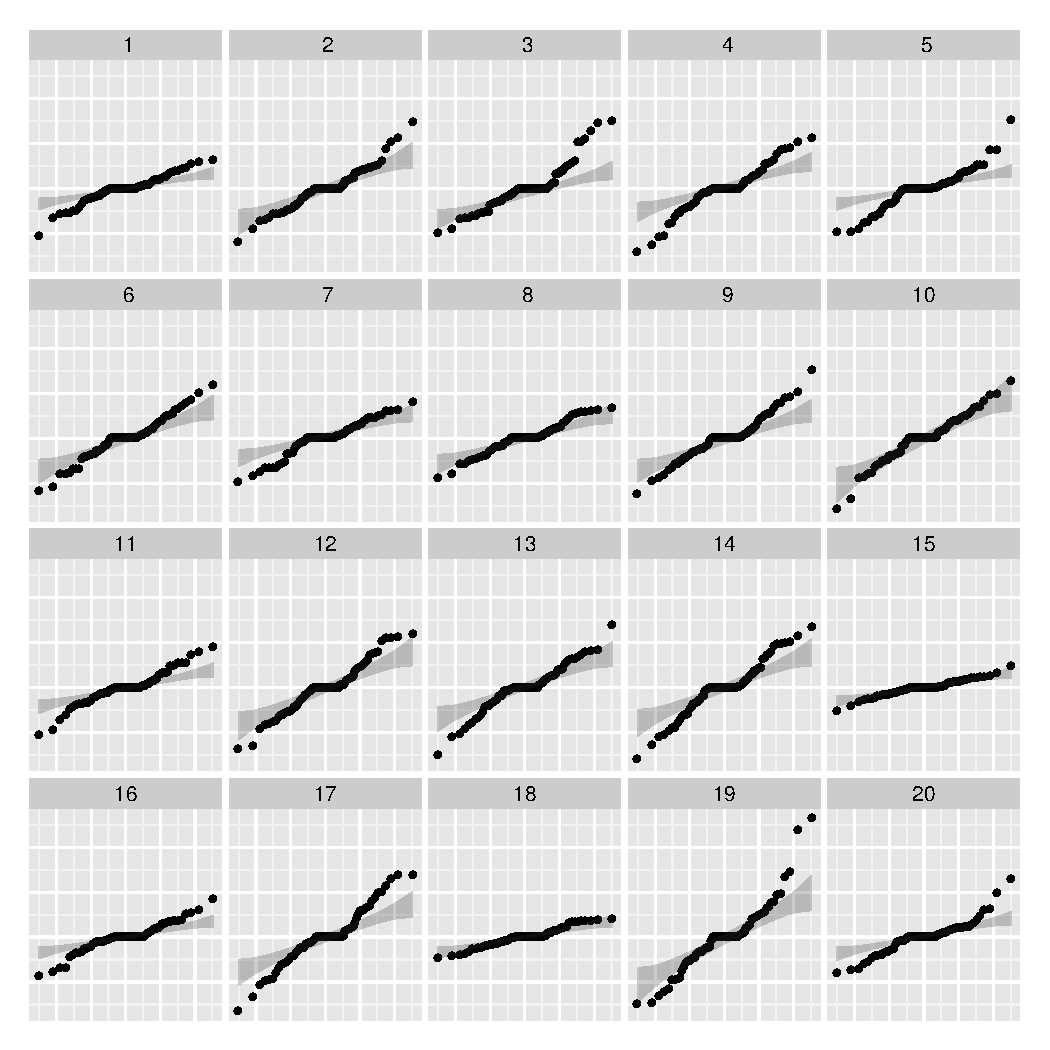
\includegraphics[width=0.8\textwidth]{radontranef-19.pdf}
	\caption{\label{fig:qqlineup-t} Lineup  testing for normality of random slopes with error terms simulated from a $t_3$ distribution. Which of the plots is the most different? Which feature led you to your choice?}
\end{figure}


% In Figure~\ref{fig:qqlineup-t} we can identify the true plot (panel $\sqrt{49} - 1$) providing evidence that the assumption of normality is violated, which is in fact the case as the true plot was constructed from random effects simulated from a $t_3$ distribution. 
To determine whether lineups can detect distributional violations we constructed another lineup where the ``true plot'' was constructed from random effects simulated from a $t_3$ distribution. This lineup is shown in Figure~\ref{fig:qqlineup-t}. Twenty nine out of 70 observers identified the true plot in panel \#($\sqrt{49} + 3\cdot4$), providing evidence against the null hypothesis of normality.  
 The fact that we can distinguish the true plot from the null plots in Figure~\ref{fig:qqlineup-t} indicates that lineups of Q-Q plots provide an avenue for distributional assessment where conventional methods fail. Further investigation is needed to explore limitations of this approach. %, as there are undoubtably situations where this approach will be unsuccessful, but this is outside the scope of the current paper.  
 The ability of a lineup to distinguish a $t$ distribution for the random effects in the radon study shows that the approach has fewer limitations than conventional approaches, justifying our preference.
%The utility of lineups in this case relies on whether the empirical distributions of predicted random effects are expected to be different under model violations, which was the case in this example. We add this as a 

%\hhnote{ I think we should include both a positive and a negative result for the Q-Q plot tests for normality - I am including five sets each of random intercepts and random slopes for the radon study. They all turned out negative ... }



%\paragraph{Residual scatterplots/boxplots.} 
%One of the most common diagnostic plots is a scatterplot or boxplot of the residuals (either level-1 or -2) against the fitted values or an explanatory variable. Such plots are often used to check linearity of the variables included in the model and homoscedasticity of the level-1 residuals. Patterns in these plots indicate departures from the model assumptions, however, we have found that patterns seem to be detectable in properly specified models more often than in the classical linear model. This problem is more commonly seen in scatterplots. 

%\paragraph{Testing homoscedasticity across groups.}
%Residual scatterplots are often used to check the assumption of homoscedastic level-1 residuals, but such plots do no account for the potential differences in variability across groups. Side-by-side boxplots of the level-1 residuals can be used to visualize this assumption; however, unbalanced group sizes can cause artificial structure in such plots. This can be seen by considering the sampling distribution of the level-1 residual variance, which has variance $\var \left( s_i^2 \right) = \left(2 \left( \sigma_i^2 \right)^2 \right) \big/ (n_i - p_i)$ which depends on the group size. Alternatively, \cite{Raudenbush:2002} propose using a standardized measure of dispersion given by
%%
%\begin{equation}\label{eq:d}
%	d_i = \frac{\log\left( s_i^2 \right) - \left[ \sum_i (n_i - r_i) \log\left( s_i^2 \right) / \sum_i  (n_i - r_i) \right]}{\left(2 / (n_i - r_i)\right)^{1/2}}
%\end{equation}
%%
%where $s_i^2$ is the residual variance within each group and $r_i = \mathrm{rank}(\bm{X}_i)$. The test statistic is then
%%
%\begin{equation}
%	H = \sum_{i=1}^{m^*} d_i^2
%\end{equation}
%%
%which has an approximate $\chi^2_{m^*-1}$ reference distribution when the data are normal and the group sizes are ``large enough''. Here we use $m^*$ because ``small'' groups may be excluded from the calculation as small group sizes provide less reliable information about the residual variance, but this is a subjective choice. If the distributional assumptions are violated or we do not have large enough group sizes, then the approximation to the $\chi^2$ distribution breaks down.


%\paragraph{Quantile-Quantile plots.}
%Quantile-Quantile (Q-Q) plots are often used as an informal check of the distributional assumptions made on the level-1 and -2 residuals; however, an interrelationship between the residual quantities exists in hierarchical linear models that can render such an assessment inappropriate. Additionally, strong assumptions are required for the empirical distributions of the residuals in the hierarchical linear model to converge in probability to their true distributions \citep[Theorem 3.2 and Lemma 3.1]{Jiang:1998vt}. If these assumptions are not satisfied, then the empirical distribution of the residuals may not resemble the hypothesized distribution under a properly specified model. Consequently, Q-Q plots will often lead to erroneous conclusions about the distributional assumptions.


%\subsubsection{Proposals for visual inference}
%------------------------------------------------------------------------------------

%The lineup protocol presents a unified approach to overcome the difficulties encountered when checking the validity of a hierarchical linear model. The only change necessary to utilize this approach to model checking is the generation of null plots, for which we use the parametric bootstrap. Consequently, the ``standard'' residuals plots can be used within this framework in order to overcome the subjectiveness of interpretation and identification of artificial structures, making visual inference a natural extension of conventional model checking. In this section we discuss several examples of lineups that we have found useful for model checking; however, we do not intend to present an exhaustive overview.

%First we consider investigating the appropriateness of a hierarchical linear model based on plots of residuals against explanatory variables. Such plots are appropriate to check the assumptions of linearity and homoscedasticity at each level of the model. The lineup in Figure~\ref{fig:constvar1} was chosen to test the homoscedasticity of the level-1 residual variance across levels of (standardized LRT scores)$^3$. Here, the true plot (panel $2^3-3$) is indistinguishable from the null plots indicating that there is no evidence that the level-1 residual variance is non-constant across the values of (standardized LRT scores)$^3$. While this conclusion is apparent from the lineup, we believe this is not the case if the true plot is considered separately. In this case, an analyst might believe that the level-1 residual variance decreases as (standardized LRT scores)$^3$ increases, which, based on the lineup, is simply artificial structure. 
% 
%\begin{figure}
%	\centering
%	\includegraphics[width=\textwidth]{normexam_constvar_lineup5.pdf}
%	\caption{\label{fig:constvar1} Lineup of 20 scatterplots of level-1 residuals against (standardized LRT)$^3$ used to test the assumption of homogeneous level-1 residual variance.  Which is the real plot?}
%\end{figure}
%
%While lineups such as Figure~\ref{fig:constvar1} address the assumption of homogeneous level-1 residual variance, they do not speak to the assumption of homogeneous level-1 residual variance across all groups. To do this we propose using a lineup of boxplots for each group ordered by their interquartile range (IQR), which we have come to call a ``cyclone'' plot. Figure~\ref{fig:badcyclone} shows a lineup of cyclone plots for 66 patients in a longitudinal study investigating the ability of Methylprednisolone to treat patients with severe alcoholic hepatitis (see Section~\ref{data:ahd} for details). The true plot (panel $2^3-3$) is easily identified from the field of null plots revealing heteroscedasticity across groups that was not detected by other plots. In this longitudinal study each subject was observed at most 5 times, with 19 subjects dropping out of the study early. Due to the small group sizes, the $\chi^2$ approximation used by the numeric approach suggested by \cite{Raudenbush:2002} is inappropriate, so conventional testing would be forced to rely on simulation, which is computationally more demanding than the generation of 19 null plots.
%
%
%\begin{figure}
%	\centering
%	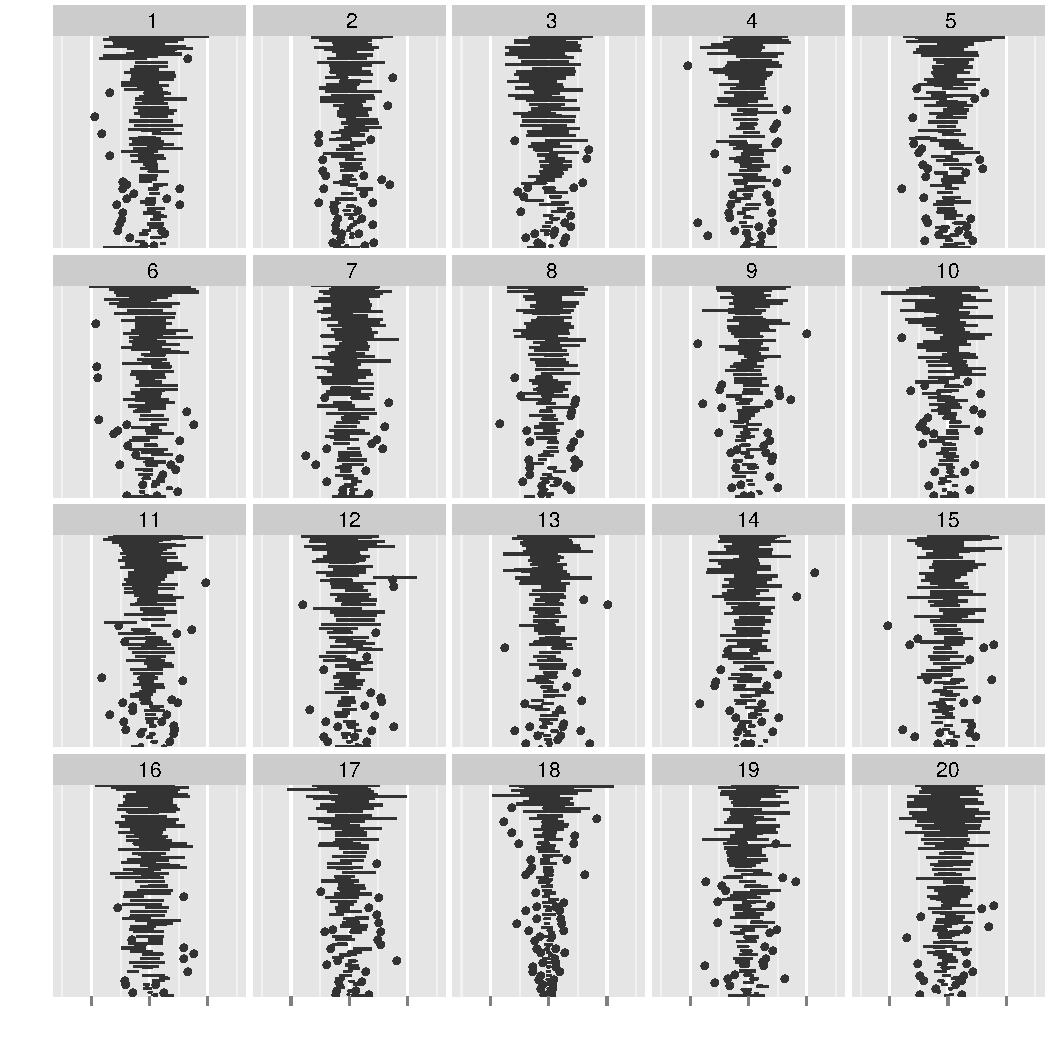
\includegraphics[width=\textwidth]{ahd_badcyclone5.pdf}
%	\caption{\label{fig:badcyclone} Lineup of 20 boxplots (ordered by IQR) of level-1 residuals used to test the assumption of homogeneous level-1 residual variance.  Which is the real plot?}
%\end{figure}
%
%\begin{figure}
%	\centering
%	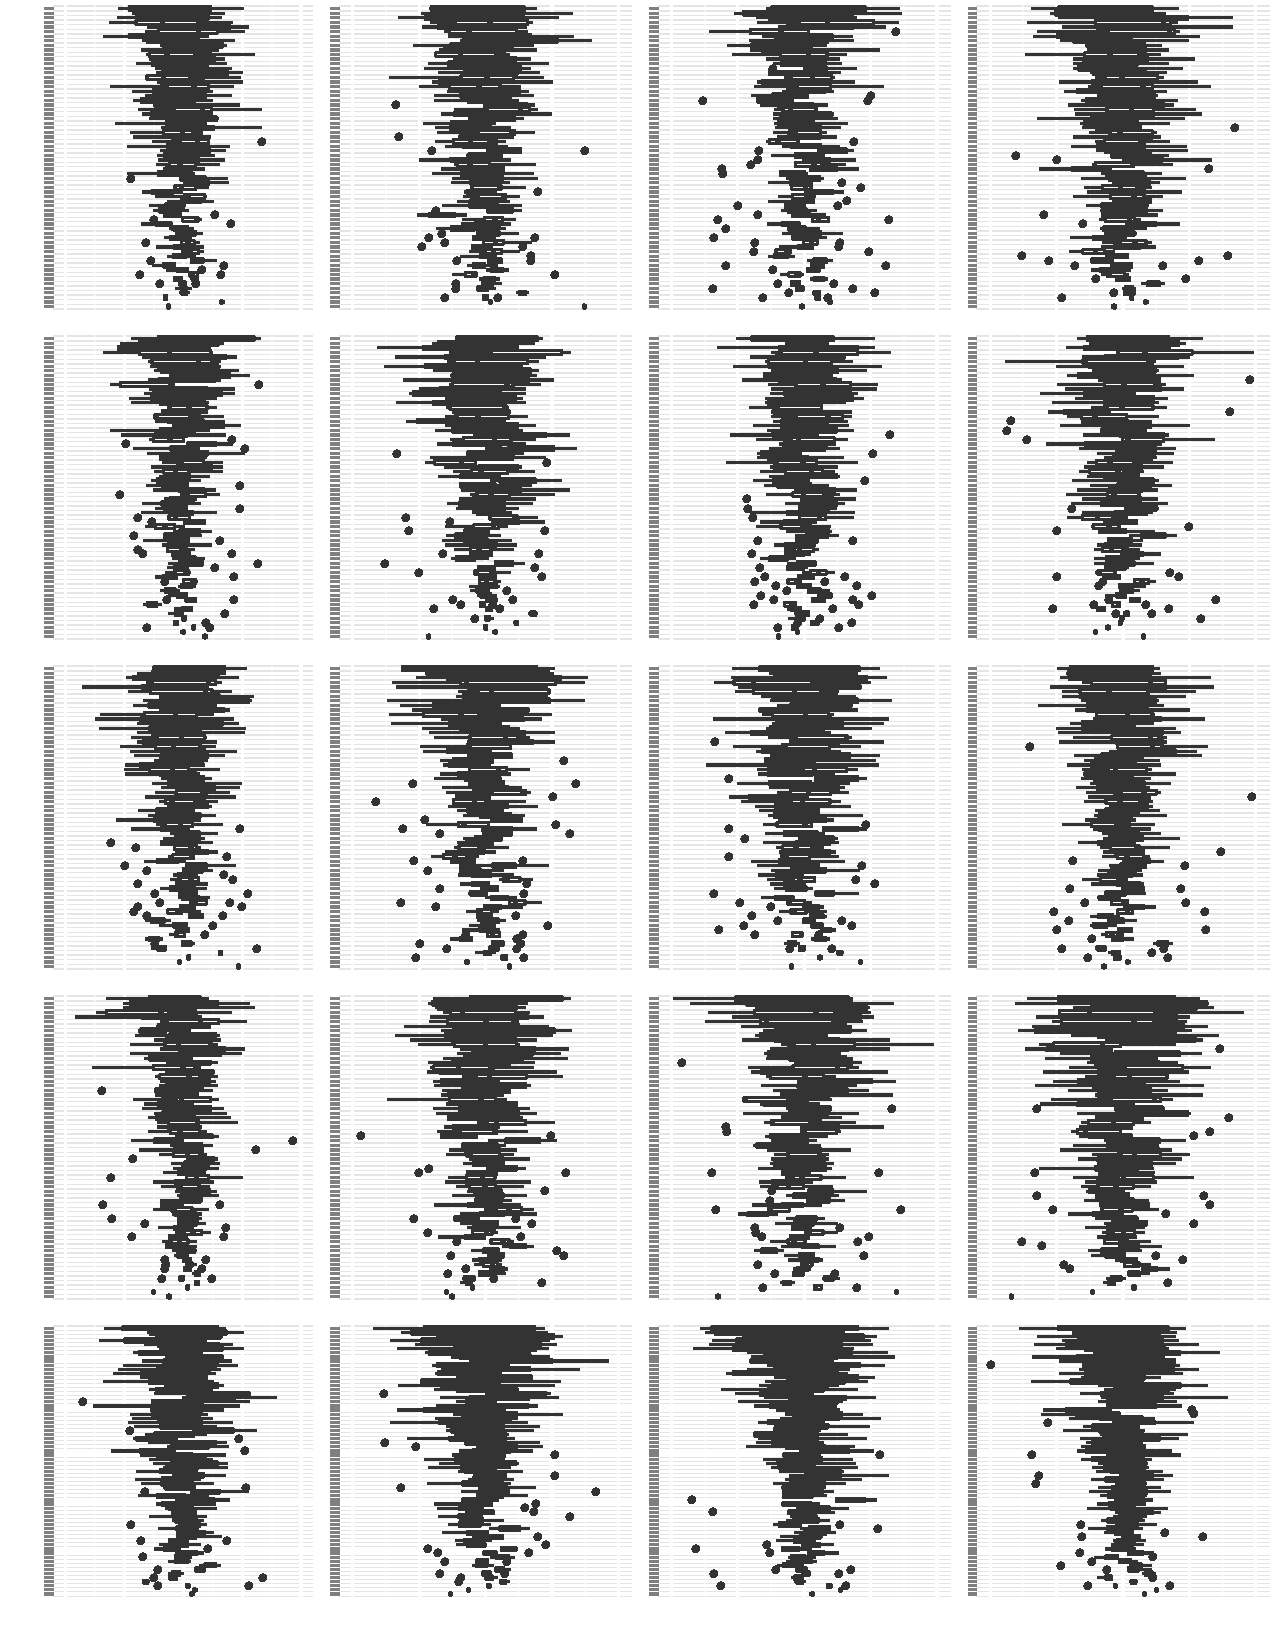
\includegraphics[width=\textwidth]{ahd_goodcyclone13.pdf}
%	\caption{\label{fig:goodcyclone} Lineup of 20 boxplots (ordered by IQR) of level-1 residuals used to test the assumption of homogeneous level-1 residual variance.  Which is the real plot?}
%\end{figure}


%Finally, the lineups presented in Figures~\ref{fig:qqlineup-norm} and \ref{fig:qqlineup-t} illustrate the use of lineups to test the distributional assumptions in a hiearachical linear model. Both lineups present simulated Q-Q plots of predicted random effects following the design of the radon study (see Section~\ref{data:radon} for details), in which group sizes were very unbalanced and there was a high degree of shrinkage. Confidence bands based on the normal distribution were applied to each lineup and reveal that the empirical distribution of the predicted random effects---both for the null plots and true plots---does not align with a normal distribution. While such confidence bands show the relationship of the predicted random effects to the hypothesized distribution, it is known that this is an ill conceived comparison in many cases; however, the lineups are not comparing the predicted random effects the normal distribution, but rather are comparing the empirical distribution of the random effects between null and observed plots. Consequently, the conclusions drawn from the lineups relate to evidence of consistency between the true plot and what is expected under a properly specified model. For example, the true plot in Figure~\ref{fig:qqlineup-norm} (panel $2^5 - 5$) is indistinguishable from the null plots, indicating no evidence of a violation of normality, but compared only to the normal distribution in a single Q-Q plot would be identified as a violation. In Figure~\ref{fig:qqlineup-t} we can identify the true plot (panel $\sqrt{49} - 1$) providing evidence that the assumption of normality is violated, which is in fact the case as the true plot was constructed from random effects simulated from a $t_3$ distribution. The fact that we can distinguish the true plot from the null plots in Figure~\ref{fig:qqlineup-t} indicates that lineups of Q-Q plots provide an avenue for distributional assessment where conventional methods fail. Further investigation is needed to explore limitations of this approach, as there are undoubtably situations where this approach will be unsuccessful, however, this is outside the scope of this paper.  The ability of a lineup to distinguish a $t$ distribution for the random effects in the radon study shows that the approach has fewer limitations than conventional approaches, justifying our preference.
%%The utility of lineups in this case relies on whether the empirical distributions of predicted random effects are expected to be different under model violations, which was the case in this example. We add this as a 
%
%
%\begin{figure}
%	\centering
%	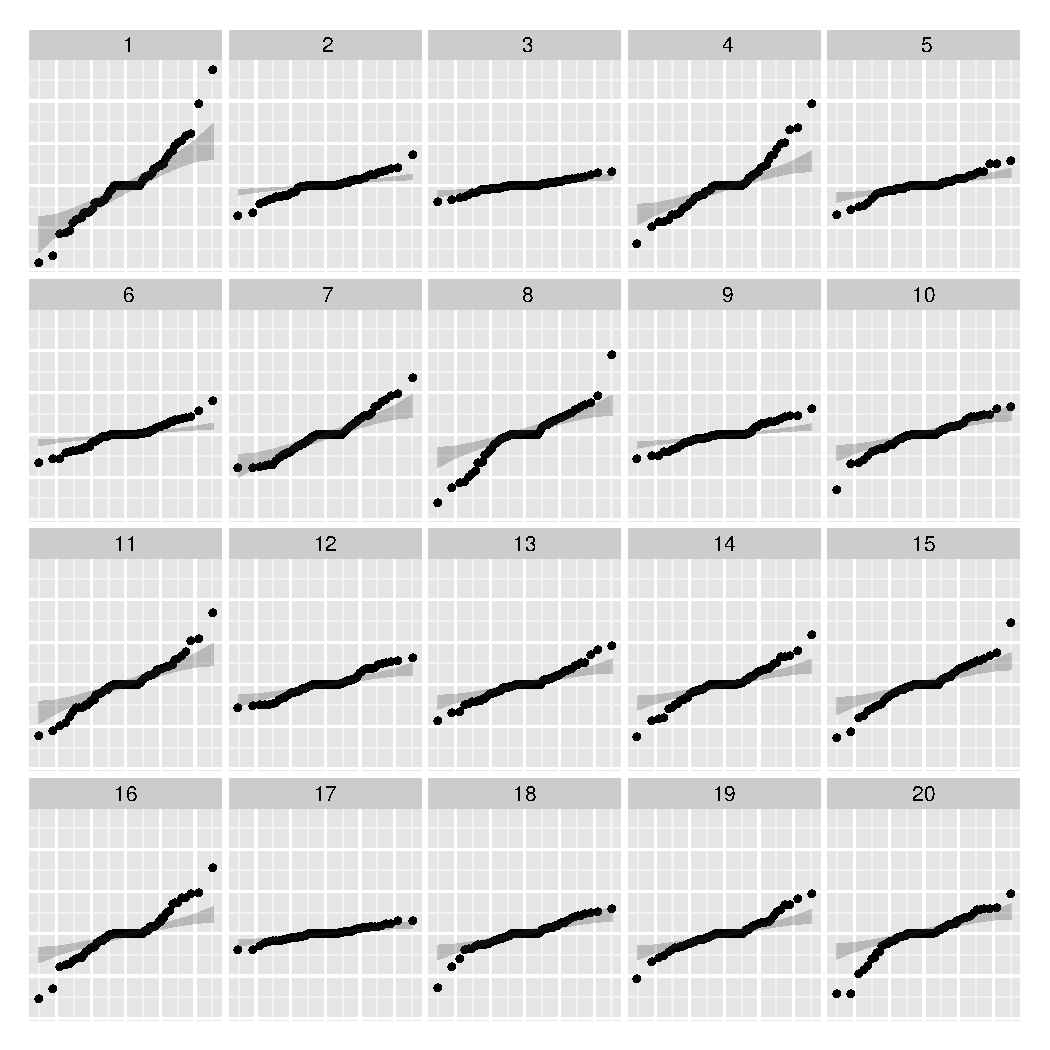
\includegraphics[width=\textwidth]{qqplot_normranef_slope_lineup11.pdf}
%	\caption{\label{fig:qqlineup-norm} Lineup of 20 normal Q-Q plots for the predicted random slope.  Which is the real plot?}
%\end{figure}
%
%\begin{figure}
%	\centering
%	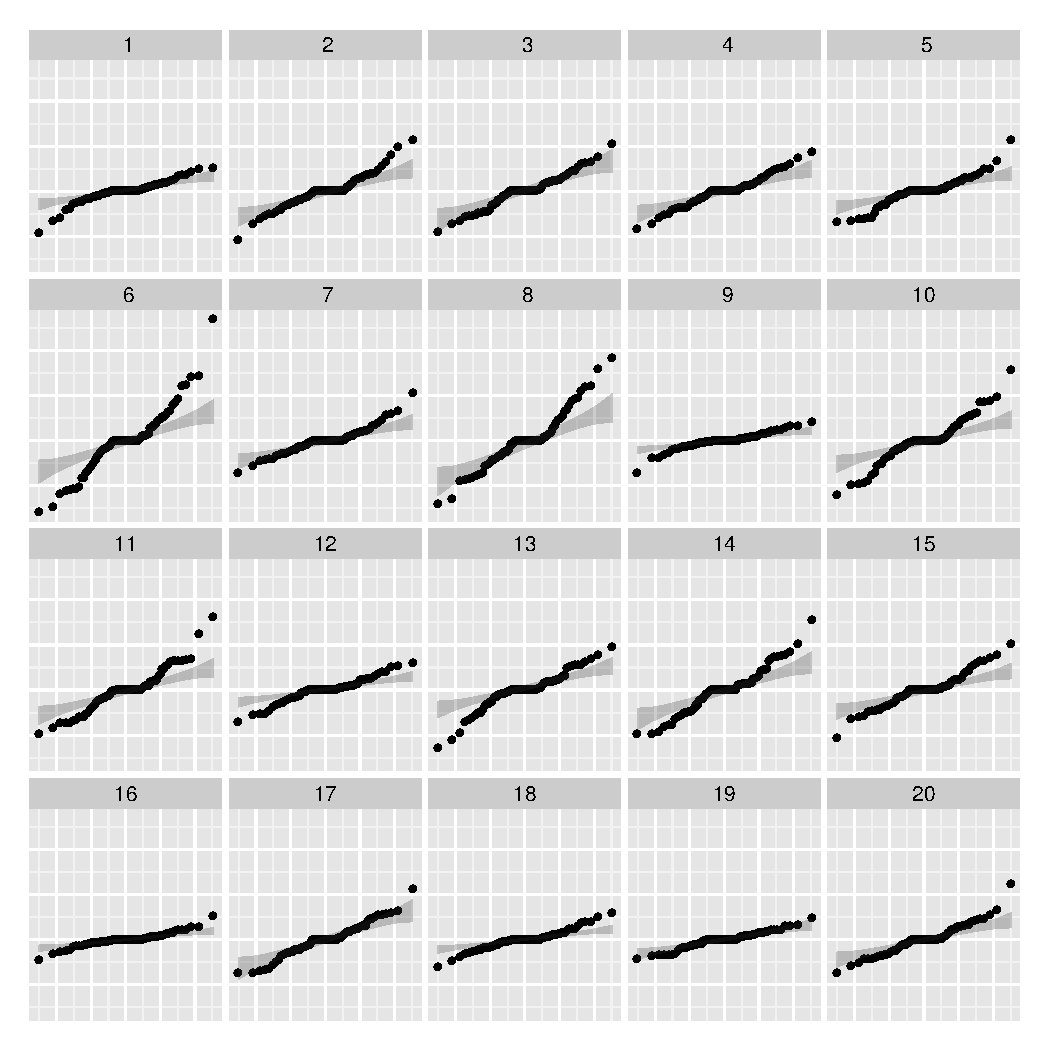
\includegraphics[width=\textwidth]{qqplot_tranef_slope_lineup6.pdf}
%	\caption{\label{fig:qqlineup-t} Lineup of 20 normal Q-Q plots for the predicted random slope.  Which is the real plot?}
%\end{figure}
%
%
%\todo[inline]{Should the below section headings be deleted?}
%
%%------------------------------------------------------------------------------------
%\section{Visual inference for hierarchical linear models}
%%------------------------------------------------------------------------------------
%
%In this section we discuss how visual inference can be implemented to conduct common tests for hierarchical linear models and to avoid misinterpreting residual plots. 
%
%
%\subsection{Model selection}
%%------------------------------------------------------------------------------------





%\begin{figure}
%	\centering
%	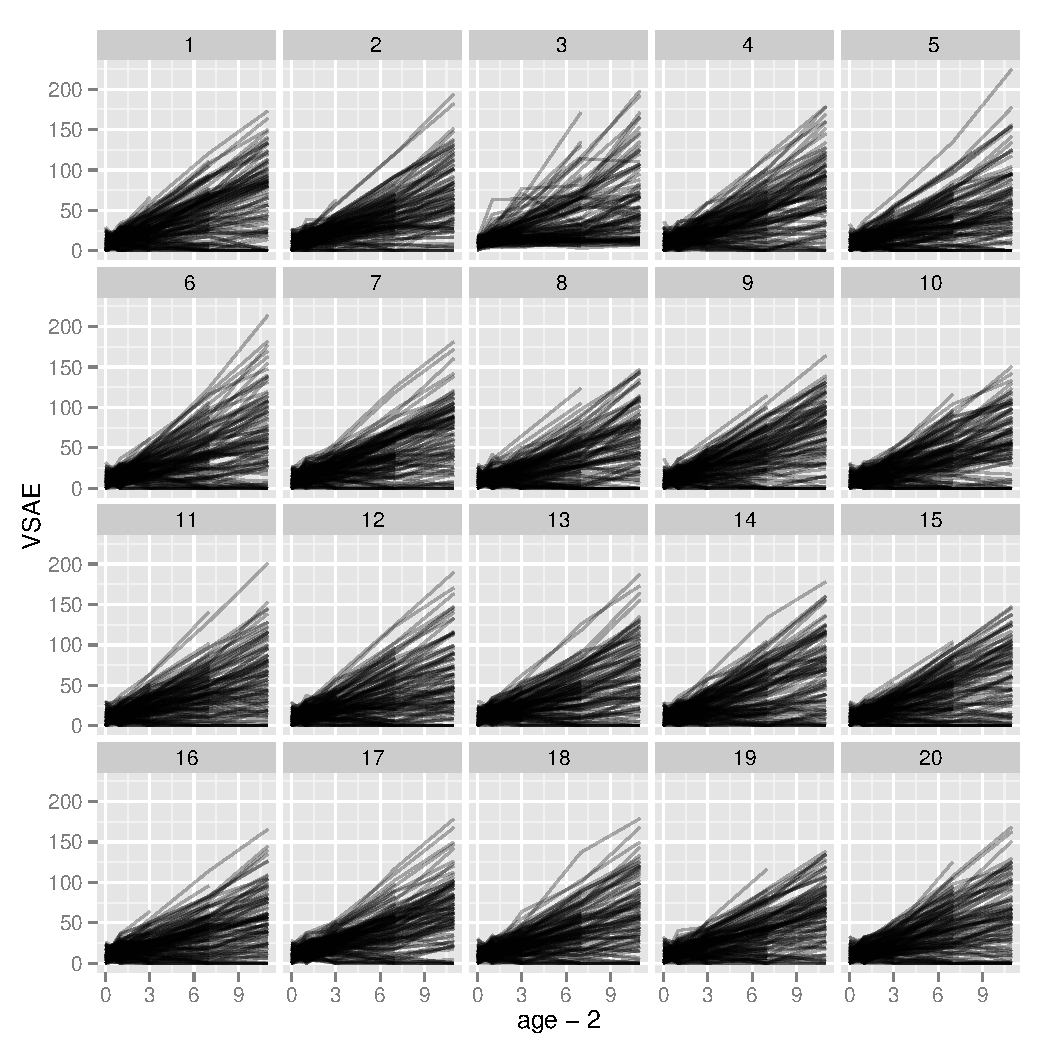
\includegraphics[width=\textwidth]{ranef1_lineup3.pdf}
%	\caption{\label{fig:lineup-ranef1} Lineup testing whether the random slope for $(\text{age} - 2)$ is sufficient, or if additional random effects are needed. These 20 plots display a child's VSAE trajectory. Which is the real plot?}
%\end{figure}
%
%\begin{figure}
%	\centering
%	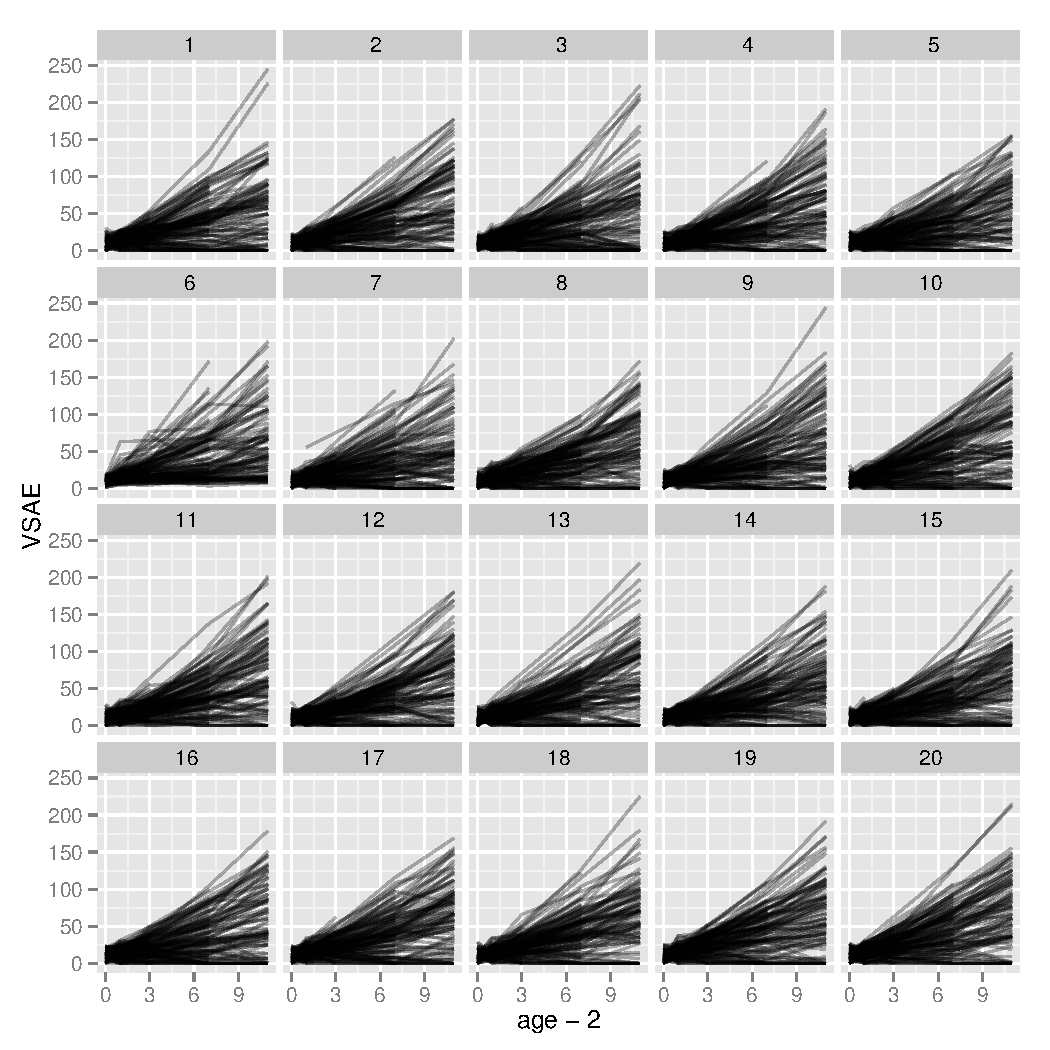
\includegraphics[width=\textwidth]{ranef2_lineup6.pdf}
%	\caption{\label{fig:lineup-ranef2} After adding a random effect for $(\text{age} - 2)^2$ we can construct the same lineup to see if we have a sufficient representation of the relationship between VSAE and age. These 20 plots display a child's VSAE trajectory. Which is the real plot?}
%\end{figure}


%\subsection{Model checking}
%%------------------------------------------------------------------------------------
%
%Include:
%\begin{itemize}
%\item Checks for level-1 and -2 heteroscedasticity -- cyclone plots, residuals vs. predictors
%\item Linearity
%
%\end{itemize}
%

%\todo[inline]{Below is a list of some initial ideas.}
%%------------------------------------------------------------------------------------
%\section{}
%%------------------------------------------------------------------------------------
%Applications of hierarchical models:
%\begin{itemize}
%\item Education -- students nested in classes nested in schools
%\item Interviewer research -- respondents nested in interviewer (Hox 1994)
%\end{itemize}
%
%Situations to consider:
%\begin{itemize}
%\item Residual analysis
%	\begin{itemize}
%	\item Unbalanced sample sizes introduces structure
%	\item Using raw rather than standardized residuals can introduce structure
%	\item This could help avoid using theoretical cutoffs for statistics used in the detection of outliers and influential points. \cite{Longford:2001wy} discusses numeric simulation-based diagnostics for outlier and makes some good points about how the theoretical distributions of these statistics are: (1) hard to calculate theoretically in many situations; (2) are based on a unit being randomly selected, as opposed to selected after an inspection of the data.
%	\end{itemize}
%
%\item Comparison of random effects -- \cite{Morrell:2000ve} discuss lines in plots of random effects appear when there are groups with a large amount of pooling (shrinkage)
%
%\item Exploratory modeling
%	\begin{itemize}
%	\item Considering a variable for inclusion in the model as a fixed effect
%	\item The need for/utility of additional random effects
%	
%	\end{itemize}
%
%
%\end{itemize}

%------------------------------------------------------------------------------------
%\section{Critical Discussion of visual inference results}\label{sec:results}
%------------------------------------------------------------------------------------

%------------------------------------------------------------------------------------
\section{Discussion and Conclusion}\label{sec:conclusion}
%------------------------------------------------------------------------------------

We have presented a graphical approach to model selection and diagnosis, using lineups constructed by simulation from the model. % fit to the true data. 
Lineup tests provide us with the framework to test hypotheses and also allow a  subsequent exploration of the plots in the lineup  for additional insight into the data structure. This approach relies  on the simulation process, the design of the graphics created, and observers, but avoids the reliance on asymptotic reference distributions; thereby circumventing the pitfalls of many commonly used tests. 
%It is important to note that simulation-based diagnostics for linear mixed-effects models have been discussed previously \citep{Longford:2001wy}, but graphical diagnosis was not the focus. A key advantage of the graphical approach is that fewer simulations are required, greatly reducing the computational burden of simulation-based diagnostics.

%\hhnote{now we need to say something on each of the pieces that lineups rely on}

%With independence from asymptotics gained, we have  to pay attention to each of the dependencies of graphical testing a bit more:
The graphical approach is relatively new, and involves working with human observers recruited on the web. There is a vast experience in statistics in engaging subjects in a traditional lab setting, where researchers are closely engaged with the experiment. With MTurk, researchers are working with subjects in a long distance relationship, and there are some participants who will try to ``game the system''. Nevertheless, results thus far are promising: experiments replicated in both environments, a replicate of the  study by \citet{cleveland:1984} using the MTurk service \citet{heer:2010} achieved matching results, and \citet{kosara:2010} found similar results between a lab study and one performed using MTurk.


Design of plots is important---some designs are better for revealing anomalies than others. At a population level, the results obtained from the same plot design are very stable. %This is reassuring and allows us to introduce the concept of power of tests into visual inference. 
In this paper design choices were made using best judgment based on  experience and results from cognitive psychology. As more studies are conducted more about the power of designs for model diagnostics will be learned, enabling more informed decisions about best practices \citep{infovis:2012}.


As with constructing surveys, avoiding leading questions is very importatnt. Mostly, the questions are very generic, asking observers to pick the plot with the most different features. Contextual information, such as labels, axis tick marks, and titles, are removed to avoid subjective bias. Care is taken, in constructnig lineup sequences and different plot designs, so that observers see the data only once. Because of the finite nature of the comparisons, multiple replications of lineups are constructed with different sets of $m-1$ null plots. In our studies five replicates were used.

%Further, we have to be careful in the application of lineup tests to maintain unbiasedness of observers. Biasing observers is relatively easy, but it also easy to avoid. We have to avoid leading questions (in our study we instead asked observers to pick the plot with the most different features), we need to make sure to remove any information from lineups that might identify the context, such as labels, axis tick marks, and titles to avoid expectation error \citep{meilgaard}, and we have to  ensure that multiple views of the same data are shown to different observers (such as in the testing sequence of Figures~\ref{fig:fanned} and~\ref{fig:fanned2} or the different designs of Figures~\ref{fig:constvar2} and~\ref{fig:constvar2.bp}).
 
%One of the advantages of visual testing using the lineup protocol is that in practice its results are decisive, resulting in $p$-values that are either very small or very close to 1; thus, decisions are rarely dependent on the exact choice of significance level. We have to be aware of the variability that is brought into the test by the choice of null plots. These $m-1$ plots are all that represent the null distribution, which is theoretically made up of infinitely many representatives. We are bound to see some ``odd'' null plots just by chance. Their influence on an individual lineup is then much higher than their nominal probability, and  affects the number of times the data plot is picked by observers. In the study underlying this paper we have accommodated for this variability by using five sets of null plots for each testing situation, and report only the $p$-value based on the combined situation.

By asking observers for the distinguishing feature(s) of the plot they chose,  graphical tests also provide us with information about the alternative hypothesis. This allows us to group responses by reasons for rejection and assess individual sub-hypotheses. In particular, it enables us to further investigate different types of errors. For example, in Figure~\ref{fig:qqlineup-t} we observed participants choosing plots for showing the ``most straight line'' or ``closest fit'' to the line of the theoretical distribution. This is why we failed to reject (type II error) in lineups 3 and 5 of this testing situation.
Similarly, we can also identify  type III errors \citep{mosteller:1948}, where we reject the hypothesis for the wrong reason, based on the reasons given by participants for their choice.


A further benefit of using the graphical framework for testing is that graphics adapt relatively well to big data situations \citep{unwin:million}. This provides us with a viable approach to assess practical relevance of a result versus results that show statistical significance purely based on the dimension of the problem. Barring bad design choices, graphical tests allow us to judge practical relevance of a result as ``If we do not see it, it might be there but not be relevant.'' 
  
%\hhnote{approach to practical relevance versus statistical significance: if we see it, it is there}  


Throughout this paper we have provided examples of graphical diagnostics that we have found to be useful. Many situations, such as outlier detection, were not discussed in this paper. This omission was not because we overlooked these diagnostic situations, but because an exhaustive list is impossible. Based on the examples and discussion throughout this paper, and the examples it builds upon \citep{Buja:2009hp, mahbub:2013}, we believe the approach can be easily adapted.

The diagnostics in this paper draw from various sources. Some of the diagnostics presented here, are well known diagnostic  tools, such as Q-Q plots or  scatterplots of residuals with trend lines as suggested by \citet{Cook:1999} for ordinary least squares regression. Some diagnostics are suggestions from the literature specific to mixed effects models. An example of a new diagnostic addressing a  practical need are the cyclone plots of Figure~\ref{fig:badcyclone}. The overarching purpose of  these examples is to show graphical diagnostics in a wide variety of situations, that all need special consideration in conventional hypothesis test, but that all fit within the same graphical inference framework.

%\hh{We do not intend for this paper to include an exhaustive discussion of all possible tests or testing situations, but rather we include some suggestions of specific diagnostics to alleviate some of the problems inherent to mixed effects models.   We hope to encourage  readers to use their own favorite graphical diagnostics for a lineup of their very own when they next diagnose a model. }


%\alnote{I think it would be useful to expand this paragraph to include a more comprehensive discussion of when we would use MTurk in practice, when we would go ask colleagues their opinions, etc. I think would clarify the process, which, as I saw from J's reaction, can seem a little odd until you wrap your head around visual inference.}


  

%\hhnote{}
%\todo[inline]{discussion for visual inference: what could go wrong; for Amazon Turk studies use \citep{kosara:2010, heer:2010} to say that previous studies \citet{cleveland:1984} have been re-done with similar results.}



%Additionally, we have presented a more detailed look at graphical diagnostics that can be used to assess distributional assumptions. We found that, contrary to expectation, rotating the Q-Q plot to emphasize the vertical comparisons does not improve the power of the graphical test. In addition to supporting the use of the standard construction of Q-Q plots, this study provides an example of how to select a graphical diagnostic based on its estimated power. 

%\alnote{I'm not quite sure where to put this... We could add a paragraph here describing what was used, or maybe an appendix? If we put it here, should it be the last paragraph?}
%\hh{Technical implementation: R \citep{R} and packages for modeling lme4 \citep{lme4}, HLMdiag \citep{HLMDiag}, and visualizations ggplot2 \citep{ggplot2}, nullabor \citep{nullabor}, gridSVG \citep{gridSVG}. 
%Mahbub's website for experiments}

%------------------------------------------------------------------------------------
\section{Acknowledgments}
%------------------------------------------------------------------------------------
We would like to thank Mahbubul Majumder and Eric Hare, who conducted the Amazon MTurk study (\url{mahbub.stat.iastate.edu/feedback_turk11/homepage.html}). R \citep{R} was used to implement all analyses and methods discussed in this paper: lme4 \citep{lme4} and HLMdiag \citep{HLMDiag, Loy:JSS} were used for model fitting and  calculation of diagnostics, respectively.  ggplot2 \citep{ggplot2}, nullabor \citep{nullabor}, and gridSVG \citep{gridSVG} provided the basis for the visualizations.
This work was funded in part by National Science Foundation grant DMS 1007697. All studies were conducted with approval from the internal review board IRB 10-347.
%------------------------------------------------------------------------------------

%\bibliographystyle{asa}
%\bibliography{hlmviz_bib}

%\clearpage
%------------------------------------------------------------------------------------
%------------------------------------------------------------------------------------

\bibliographystyle{asa}
\bibliography{hlmviz_bib}

%------------------------------------------------------------------------------------
\clearpage
\appendix
\section{Data sets}\label{sec:datasets}
%------------------------------------------------------------------------------------

All of the data sets used in this paper are publicly available: the General Certificate of Secondary Education Exam data set is available in the R package mlmRev \citep{mlmRev}; the Dialyzer data set is available in the R package MEMSS \citep{MEMSS}; all other data sets can be found in the R package HLMdiag \citep{HLMDiag}.

\subsection{General certificate of secondary education exam data}\label{data:GCSE}

We make use of a subset of examination results of 4,065 students nested within 65 inner-London schools discussed by \cite{Goldstein:1993wm}. The original analysis explored school effectiveness as defined by students' performance on the General Certificate of Secondary Education Exam (GCSEE) in both mathematics and English. This exam is taken at the end of compulsory education, typically when students are 16 years old.  To adjust for a student's ability when they began secondary education, the students' scores on the standardized London Reading Test (LRT) and verbal reasoning group (bottom 25\%, middle 50\%, or top 25\%) at age 11. Additional information contained in the data set includes student gender, school gender, and the average LRT intake score for each school. 


\subsection{Autism study}\label{data:autism}
%------------------------------------------------------------------------------------
%\alnote{I need to pare this down.}
%Autism is a developmental disorder typically characterized by impaired communication and social skills, but there is relatively little consensus on how these abilities or disabilities change over time \citep{Anderson:2007cl, Anderson:2009in}. 
In an effort to better understand changes in verbal and social abilities from childhood to adolescence, \cite{Anderson:2007cl, Anderson:2009in} carried out a prospective longitudinal study following 214 children between the ages of 2 and 13 who had been diagnosed with either autism spectrum disorder or non-spectrum developmental delays at age 2. The Vineland Adaptive Behavior Interview survey was used to assess each child's interpersonal relationships, play time activities, and coping skills, 
%This survey is completed by the parents. 
from which the Vineland Socialization Age Equivalent (VSAE) was computed as an overall measure of a child's social skills. Additionally, expressive language development at age 2 was assessed using the Sequenced Inventory of Communication Development (SICD) and the children were classified into three groups (high, medium, or low). Assessments were made on the children ages 2, 3, 5, 9, and 13, however, not all children were assessed at each age. Additional information collected on each child includes: gender, race (white or non-white), and initial diagnosis at age 2 (autism, pervasive development disorder (pdd), or non-spectrum). We restricted attention to models concerned with the changes in social skills for subjects diagnosed with autism spectrum disorder having complete data. This results in a reduced data set of 155 children. For more detailed analyses we refer the reader to \cite{Anderson:2007cl, Anderson:2009in}.

\subsection{Methylprednisolone study}\label{data:ahd}
%------------------------------------------------------------------------------------

\cite{Carithers:1989} conducted a four week longitudinal study to investigate the effectiveness of methylprednisolone to treat patients with severe alcoholic hepatitis. The researchers randomly assigned 66 patients to receive either methylprednisolone (35 patients) or a placebo (31 patients). Over the study duration, each subject's serum bilirubin levels (in $\mu$mol/L) were measured each week, with the first measurement taken at the start of the study (week 0).

\subsection{Dialyzer study}\label{data:dialyzer}
%------------------------------------------------------------------------------------

\cite{Vonesh:1992us} describe a study characterizing the water transportation characteristics of 20 high flux membrane dialyzers, which were introduced to reduce the time a patient spends on hemodialysis. The 20 dialyzers were studied \emph{in vitro} using bovine blood at flow rates of either 200 or 300 ml/min, and the ultrafiltration rate (ml/hr) for each dialyzer was measured at seven transmembrane pressures (in mmHg). \cite{Vonesh:1992us} use nonlinear mixed-effects models to analyze these data; however, they can be modeled using polynomials in the linear mixed-effects framework \citep[Section 9.5]{Littell:2006}.

\subsection{Radon study}\label{data:radon}
%------------------------------------------------------------------------------------

The data consist of a stratified random sample of 919 owner-occupied homes in 85 counties in Minnesota. For each home, a radon measurement was recorded (in log $pCi/L$, i.e., log picoCuries per liter) as well as a binary variable indicating whether the measurement was taken in the basement (0) or a higher level (1). Additionally, the average soil uranium content for each county was available. The number of homes within each county varies greatly between counties ranging from one home to 116 homes, with 50\% of counties having measurements from between 3 and 10 homes. \cite{Gelman:2006ue} suggest a simple hierarchical model allowing for a random intercept for each county and a random slope for floor level. This is the model from which we simulate predicted random effects.

%------------------------------------------------------------------------------------
\section{Experimental Setup and Results}\label{study}
%------------------------------------------------------------------------------------
\subsection{Experimental Setup and Calculation of $p$-values}\label{sec:pvalues}
For each of the lineup designs described in the paper we constructed five replicates consisting of the same data plot and different sets of nineteen null plots for a total of 75 different lineups. These were evaluated by 487 participants in altogether 4927 evaluations. For each lineup, observers were instructed to identify the plot  most different from the set and asked what feature led them to their choice. 
These choices came in form of four suggestions (in checkboxes) and one text box for a free-form answer. For each lineup the time was taken to answer and  observers were asked for their confidence level (on a scale from 1=weak to 5=high). Observers were also asked to provide their demographics: age category, gender,  education range, and geographic location (from parts of the ip address). 

The results of the evaluations for all lineups  are displayed in Table~\ref{tab:results} and the observers' reasons for identifying plots are summarized in Table~\ref{tab:reasons}. 
The significances in Table~\ref{tab:results} are based on the number of evaluations and the times that the data plot is being identified. For that, we introduce random variable $Y$ as the  number of evaluations of a lineup in which the observer identifies the data plot. Assume that the lineup has size $m=20$, and it is shown to a total of $K$ independent observers.  Then $Y$ has a Visual distribution $V_{K, m, s=3}$ as defined in \hh{reference to technical report}, where $s$ delineates scenario III, i.e.~the same lineup is shown to all $K$ observers. The $p$-values in Table~\ref{tab:results} for each of the five replicates are calculated this way.
For the overall $p$-value, we use a simulation based approach to combine the five results. Treating the number of evaluations $(K_1, ..., K_5)$ as fixed, we simulate assessments of lineups without signal as follows: we assume that the signal in a plot is complementary to its $p$-value, which is i.i.d. $U[0,1]$ under the null hypothesis. We further assume that the probability an observer picks a  plot  is allocated proportionally to its signal. For each ``data plot'' we create five sets of null plots to be evaluated simultaneously $(K_1, ..., K_5)$ times.  
$p$-values are then based on a comparison of the sum of data picks from  five no-signal lineups and  the observed number of data picks from the actual lineups. The column on the right of Table~\ref{tab:results} shows $p$-values based on $10^5$ simulation runs.


%How did we get the data? Some information on Amazon Turk, and setup of experiments. 

%\hhnote{Data collected for each response: time taken, answer(s), confidence level and reason for choice - four suggestions in form of check boxes, one text box;
%data collected on each participant: gender, age group, education level, geography (from ip address), nickname to match responses from the same individual. }


%%------------------------------------------------------------------------------------
%\subsection{Discussion of study results} % and participants' demographics}
%%------------------------------------------------------------------------------------
%
%%All of the lineups discussed in this paper (and the two presented in Appendix~\ref{app:morelineups}) were evaluated using Amazon MTurk. All  lineups were evaluated in the same study, which we describe below.
%
%%For each of the ten lineups, five replications were constructed for a total of 50 lineups. The replications for the lineup in Figure~\ref{fig:qqlineup-t} were created by different simulations, while the replications for the remaining lineups were created by shuffling the location of the true plot and exchanging the null plots for additional simulations under the null model. For each lineup, observers were instructed to identify the plot that is most different and asked what feature led them to their choice. Overall the study was comprised of  334 participants who made 3441 evaluations. 
%
%The results show that for all but the Q-Q plots of the random slopes, enough observers identified the true plot so that we reject the null hypotheses that the data are consistent with what is expected under the null model. For the Q-Q plot of the random slopes generated by a $t$ distribution, three of the five replicates resulted in a rejection of the null hypothesis of normality. The variability in the results is explained by different ``true'' plots being simulated for each replicate. 



%\hhnote{I'm not sure how much more detail we can give here - we're in the process of writing up the exact distribution, but the vinference package on my github site already allows for a calculation of the corrected $p$-values.}
%\alnote{Can we cite the R package? Having a citation might help with this.}
%
%\hhnote{Only three out of five replicates are providing significant results against the null hypothesis.}
%
%\hhnote{Explain how we deal with five $p$-values from five lineups with the same data and different null sets }


%\hh{There are five different null sets for each data set. Throughout the paper we show lineups for the first replicate. In all of the lineups with the exception of figure~\ref{fig:qqlineup-1} observers are identifying the data plot to a degree that we have to reject the null hypotheses of the data being consistent with the null model. }
%\hh{For the radon t ranef example we have actually five different samples from a $t$ distribution in the lineups - that explains the much larger variability between the results. }

% latex table generated in R 3.0.1 by xtable 1.7-1 package
% Tue Jun  4 23:00:42 2013
\begin{table}[ht]
\centering
\caption{\label{tab:results} Overview of all lineup evaluations. Ratios comparing the number correct to the total number of evaluations are shown.  $p$-values and significances are based on the calculations as described in section~\ref{sec:pvalues}} 
\begin{tabular}{Mrrlrlrlrlrlc}
  \hline
&  & \multicolumn{9}{c}{Replicate} && Overall \\ \cline{3-12} 
\multicolumn{2}{c}{Lineup} & 1 & & 2 && 3 && 4 && 5 && $p$-values\\ 
  \hline
  

\includegraphics[width=0.05\textwidth]{examfanned-icon}&  fig.~\ref{fig:fanned} & 11/73&\hspace{-0.1in}* & 7/70&\hspace{-0.1in} & 9/65&\hspace{-0.1in}*& 13/66&\hspace{-0.1in}** & 7/72&\hspace{-0.1in} & 0.0001\\ 
 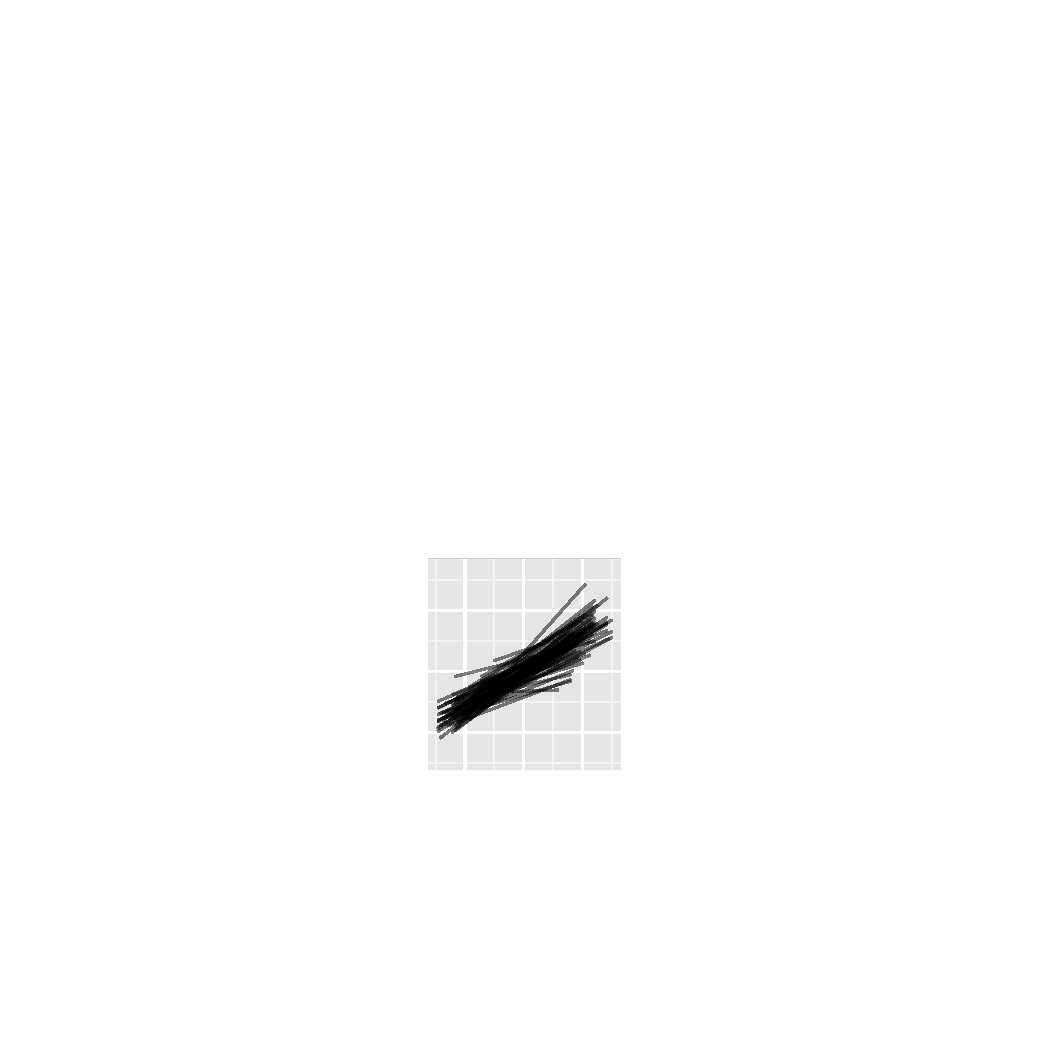
\includegraphics[width=0.05\textwidth]{exam-with-slope-icon} & fig.~\ref{fig:fanned2} & 0/64 & \hspace{-0.1in}  & 7/75 & \hspace{-0.1in}  & 11/76 & \hspace{-0.1in}* & 0/69 & \hspace{-0.1in}  & 0/60 & \hspace{-0.1in} & 0.4837 \\ 
%
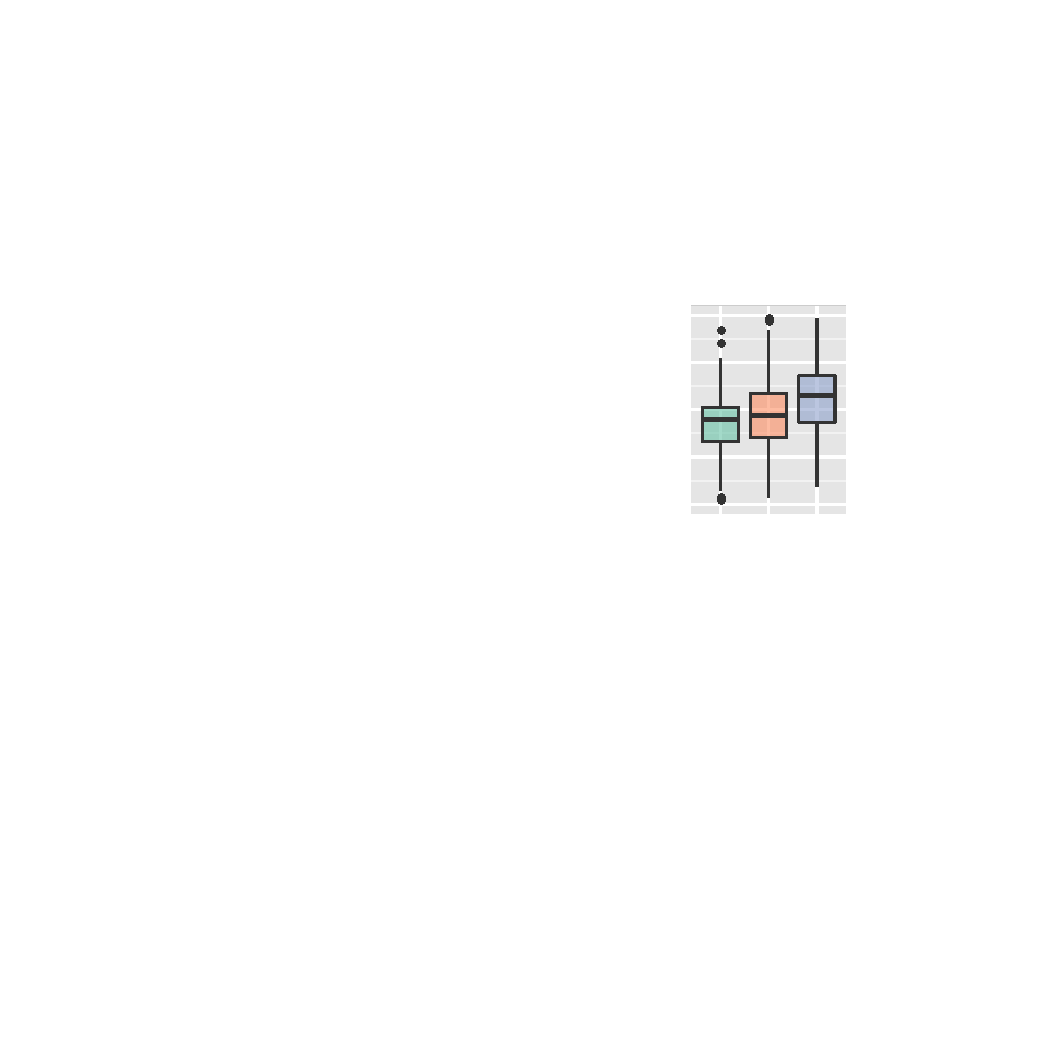
\includegraphics[width=0.05\textwidth]{autism-ordered-icon}&   fig.~\ref{fig:boxplot-ordered} & 65/74&\hspace{-0.1in}*** & 57/66&\hspace{-0.1in}*** & 62/68&\hspace{-0.1in}*** & 54/63&\hspace{-0.1in}*** & 66/76&\hspace{-0.1in}*** & $<10^{-5}$\\ 
%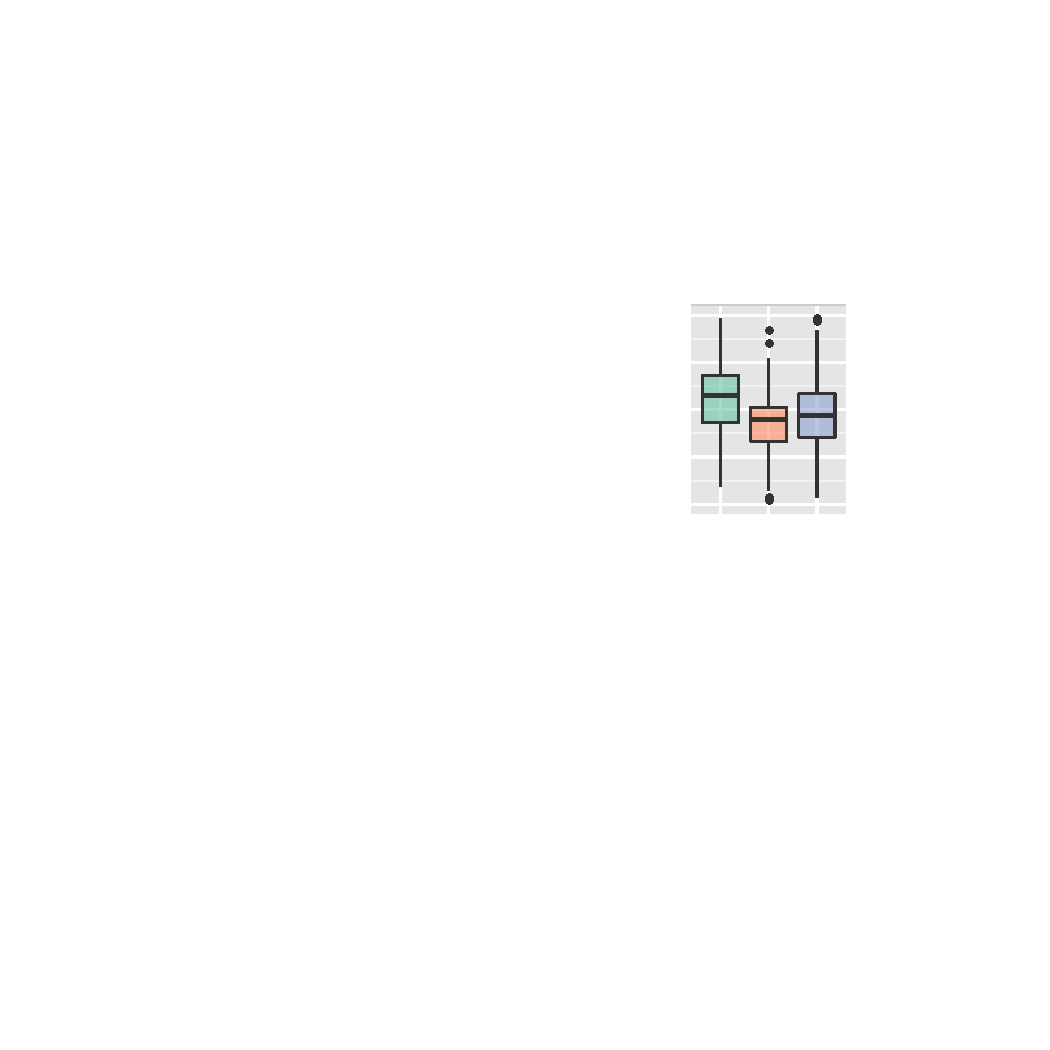
\includegraphics[width=0.05\textwidth]{autism-unordered-icon}&   fig.~\ref{fig:boxplot-unordered} & 52/54&\hspace{-0.1in}***  & 63/76&\hspace{-0.1in}*** & 70/75&\hspace{-0.1in}*** & 59/64&\hspace{-0.1in}*** & 63/70&\hspace{-0.1in}*** & $<10^{-5}$\\ 
 %
 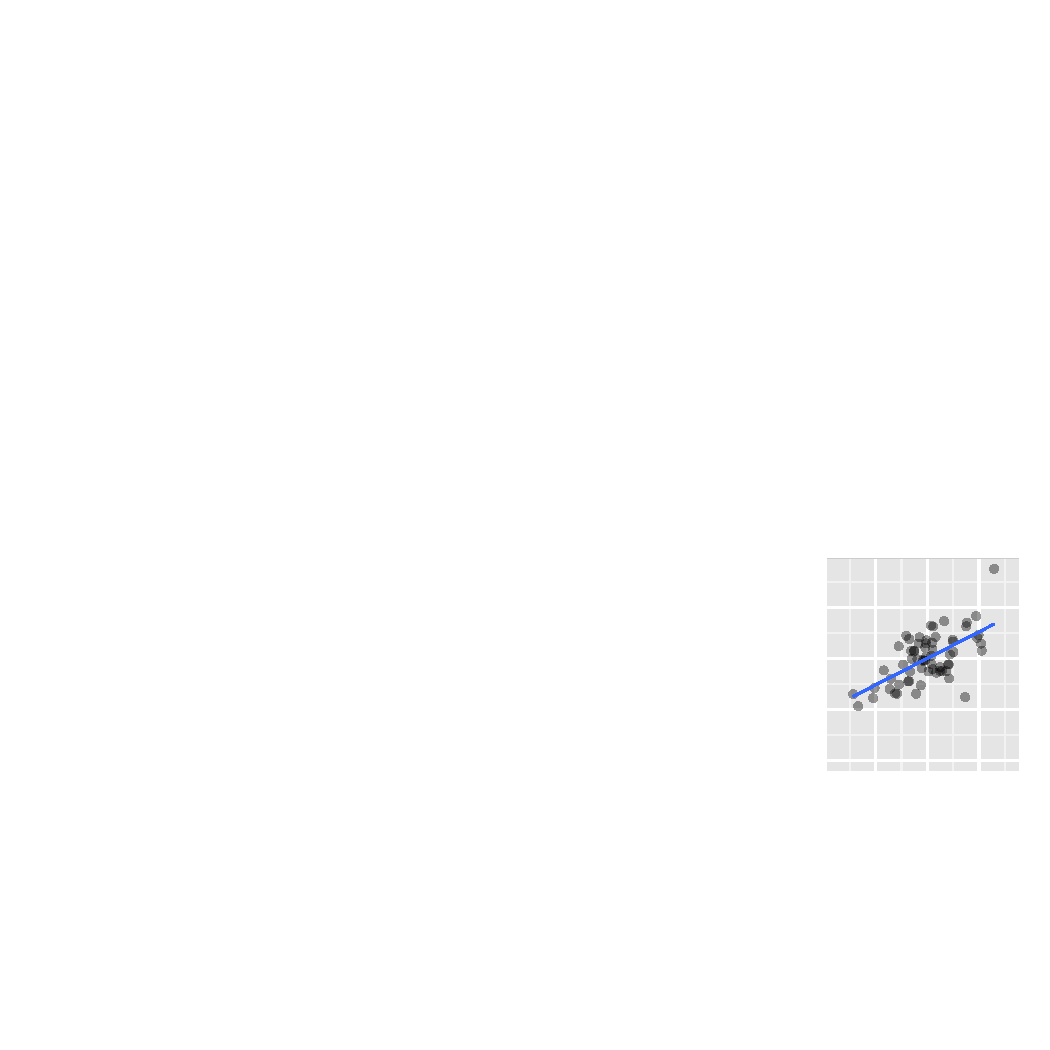
\includegraphics[width=0.05\textwidth]{examcorr-icon}&   fig.~\ref{fig:ranef-corr} & 41/69&\hspace{-0.1in}*** & 62/73&\hspace{-0.1in}*** & 31/64&\hspace{-0.1in}*** & 57/75&\hspace{-0.1in}*** & 55/67&\hspace{-0.1in}*** & $<10^{-5}$\\ 
 %
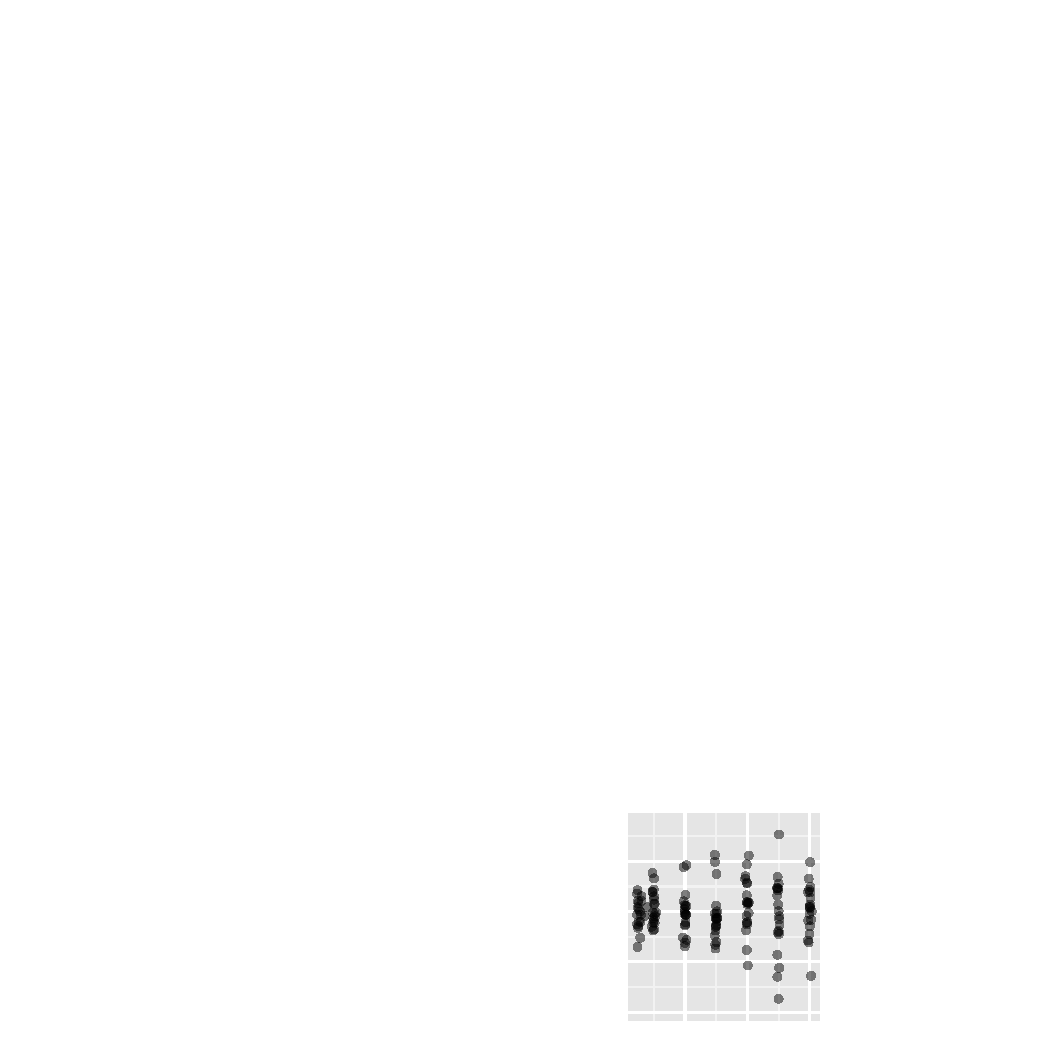
\includegraphics[width=0.05\textwidth]{dialyzerheterogeneous-icon}& fig.~\ref{fig:constvar2} & 29/85&\hspace{-0.1in}***  & 10/65&\hspace{-0.1in}* & 24/64&\hspace{-0.1in}*** & 7/60&\hspace{-0.1in}. & 13/72&\hspace{-0.1in}** & $<10^{-5}$\\ 
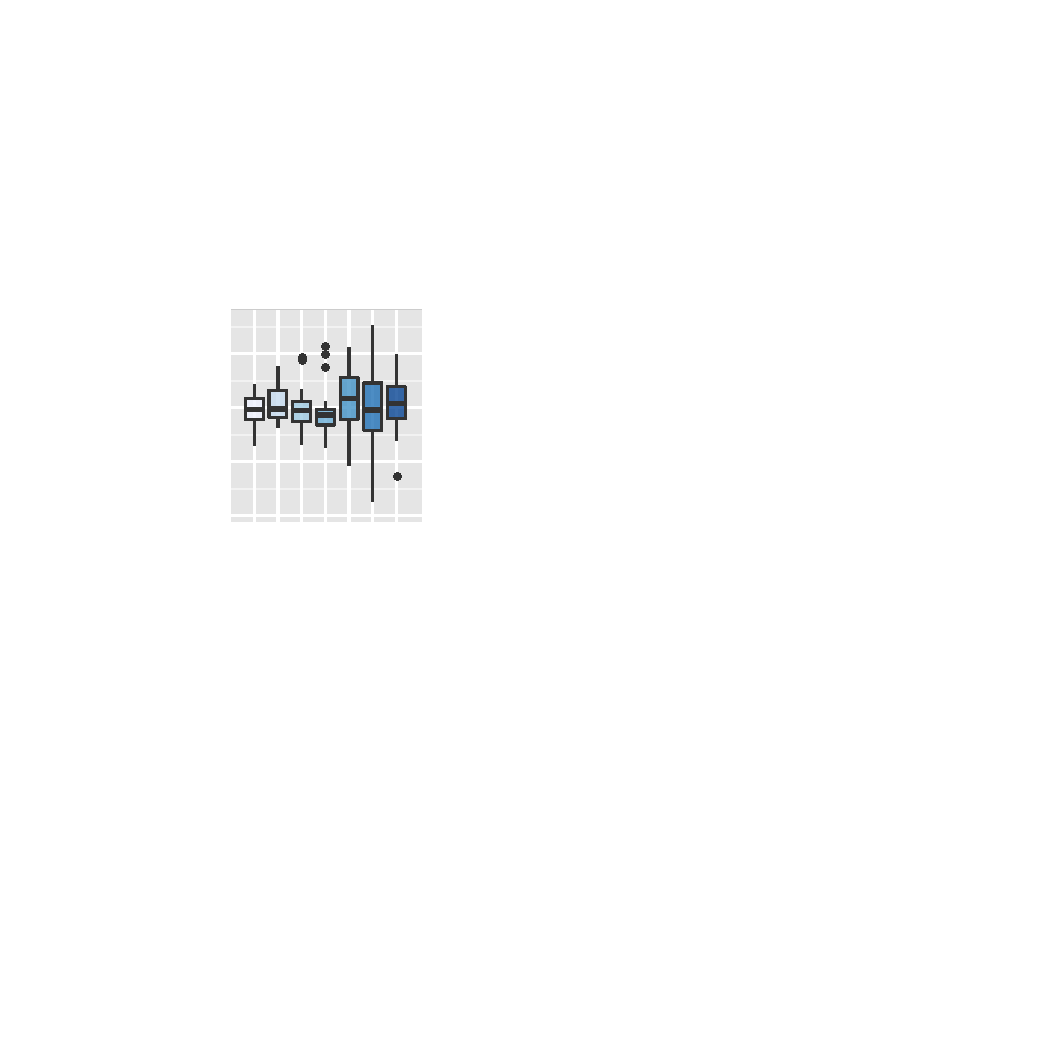
\includegraphics[width=0.05\textwidth]{dialyzerheterogeneous-bp} &  fig.~\ref{fig:constvar2.bp} & 23/70 & \hspace{-0.1in}*** & 9/74 & \hspace{-0.1in}. & 11/62 & \hspace{-0.1in}** & 31/78 & \hspace{-0.1in}*** & 25/61 & \hspace{-0.1in}*** & $<10^{-5}$\\ 
%
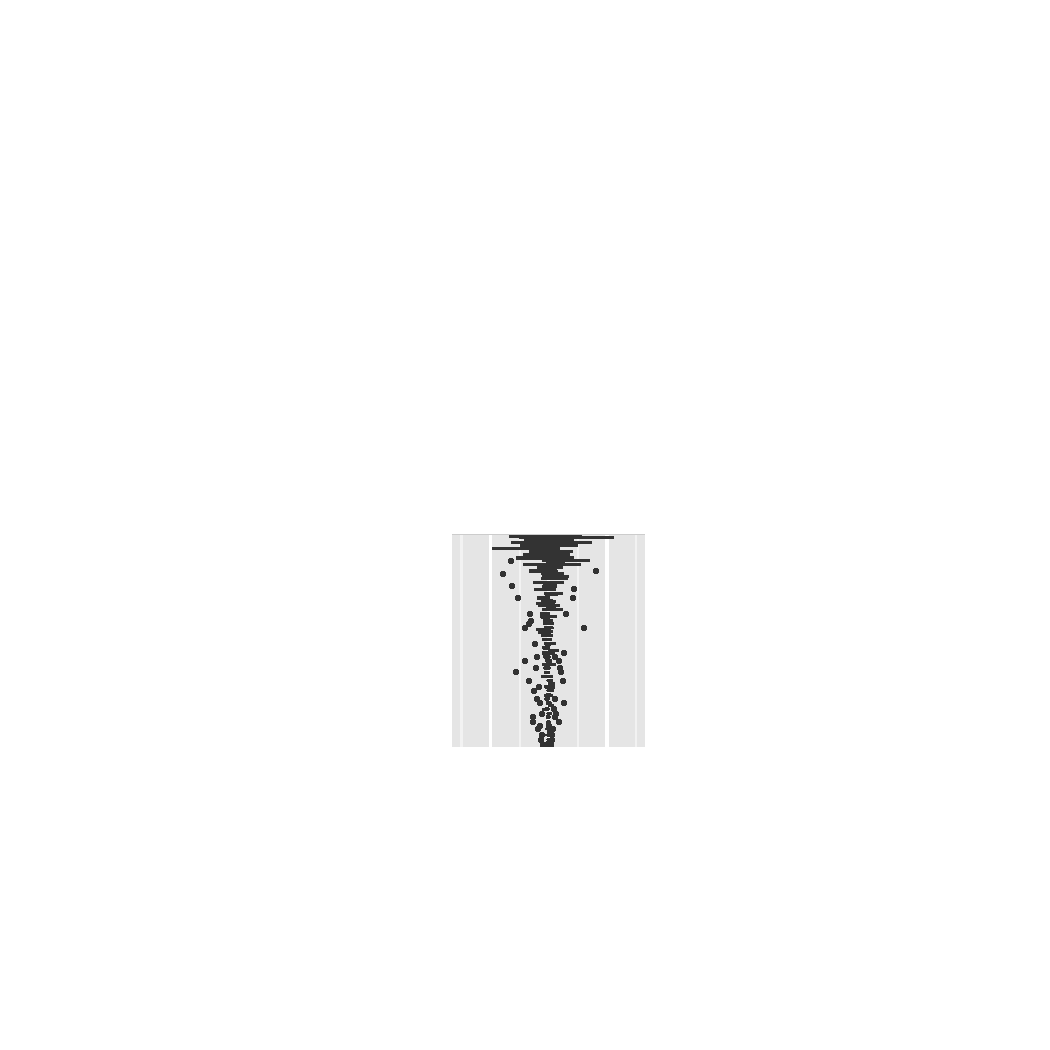
\includegraphics[width=0.05\textwidth]{cyclone-icon}&   fig.~\ref{fig:badcyclone} & 50/75&\hspace{-0.1in}***  & 44/64&\hspace{-0.1in}*** & 45/68&\hspace{-0.1in}*** & 46/76&\hspace{-0.1in}*** & 50/67&\hspace{-0.1in}*** & $<10^{-5}$\\ 
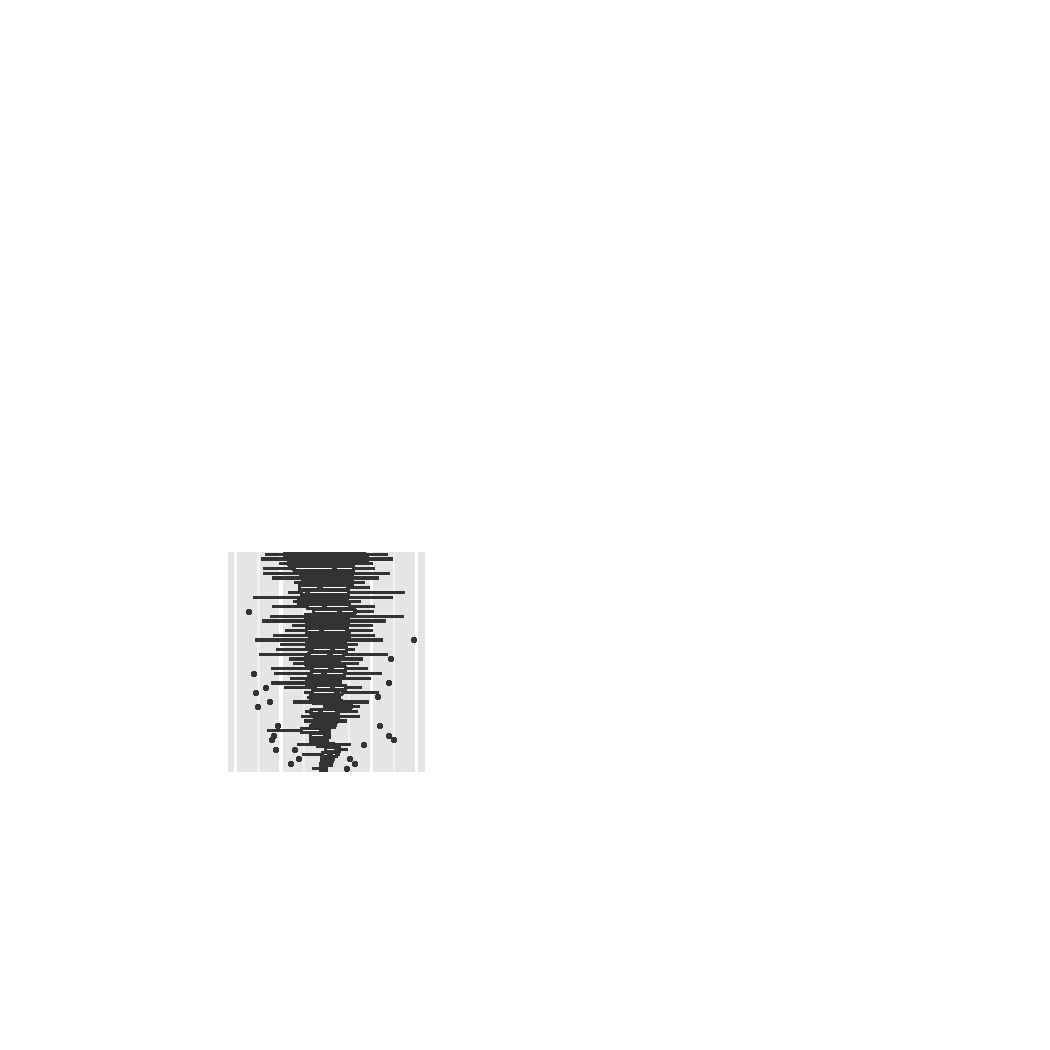
\includegraphics[width=0.05\textwidth]{cyclone-good-icon} & fig.~\ref{fig:goodcyclone}  & 1/59 & \hspace{-0.1in}  & 2/79 & \hspace{-0.1in}  & 2/68 & \hspace{-0.1in}  & 4/62 & \hspace{-0.1in}  & 1/73 & \hspace{-0.1in}  & 0.7180\\ 
%
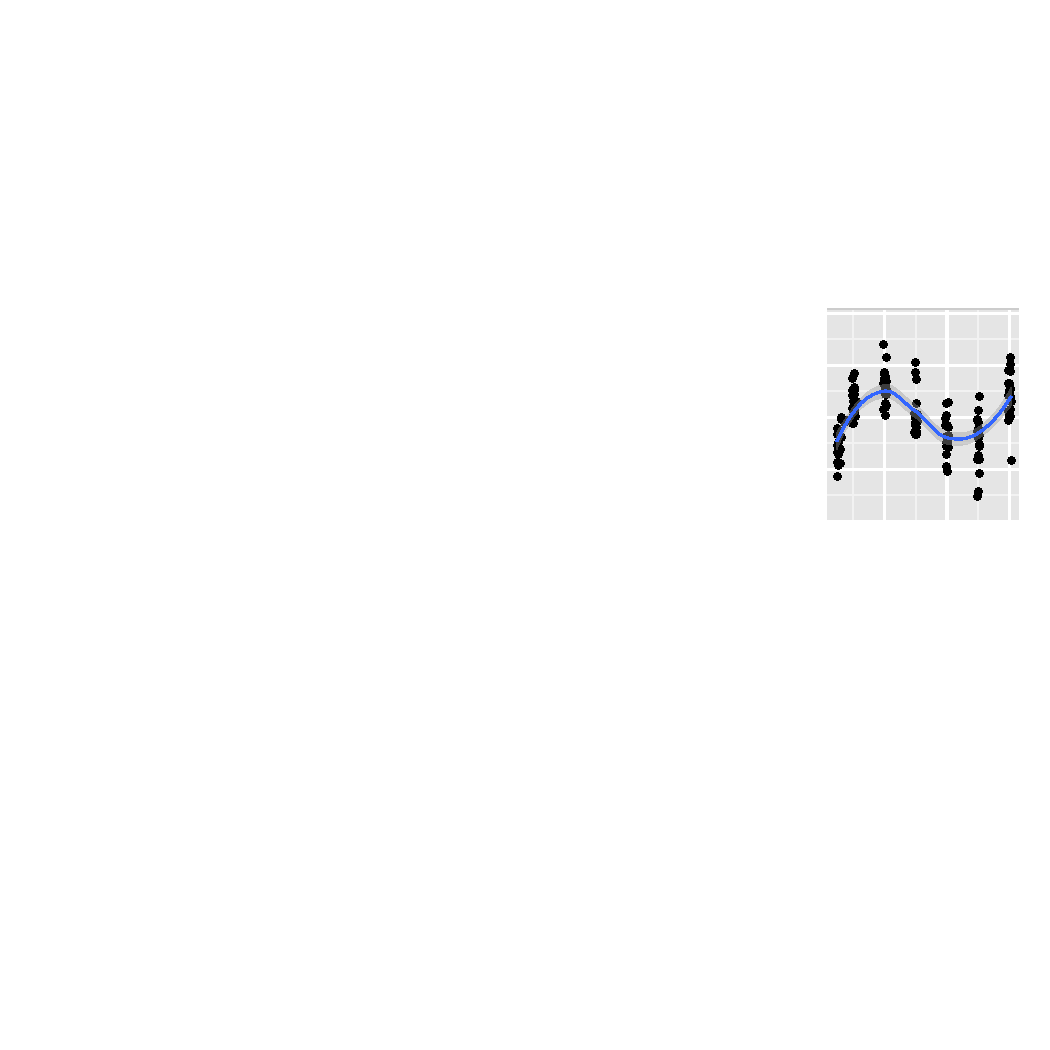
\includegraphics[width=0.05\textwidth]{dialyzernonlinear-icon}&   fig.~\ref{fig:linearity} & 60/63&\hspace{-0.1in}***  & 62/64&\hspace{-0.1in}*** & 57/60&\hspace{-0.1in}*** & 84/88&\hspace{-0.1in}*** & 66/69&\hspace{-0.1in}*** & $<10^{-5}$\\ 
%
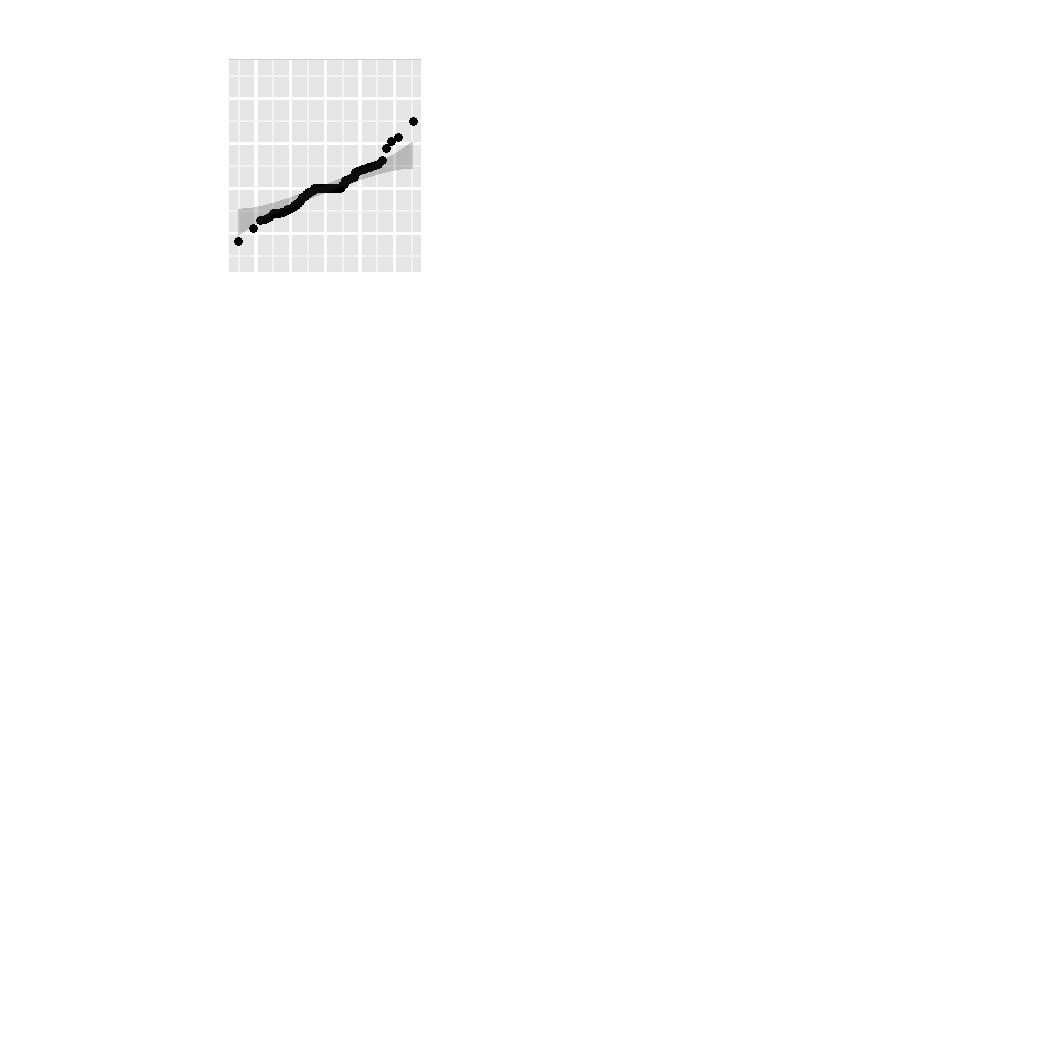
\includegraphics[width=0.05\textwidth]{radontranef-icon}&   fig.~\ref{fig:qqlineup-t} & 29/70&\hspace{-0.1in}***  & 52/79&\hspace{-0.1in}*** & 0/64& & 13/59&\hspace{-0.1in}*** & 6/74& & $<10^{-5}$\\ 
\multicolumn{2}{r}{random intercept} & 0/72 & \hspace{-0.1in}  & 1/75 & \hspace{-0.1in}  & 0/68 & \hspace{-0.1in}  & 0/75 & \hspace{-0.1in}  & 2/61 & \hspace{-0.1in} & 0.9458 \\ 
\multicolumn{2}{r}{random slope} & 0/65 & \hspace{-0.1in}  & 0/64 & \hspace{-0.1in}  & 0/68 & \hspace{-0.1in}  & 0/46 & \hspace{-0.1in}  & 0/64 & \hspace{-0.1in}  & 1.0000\\ 
%
 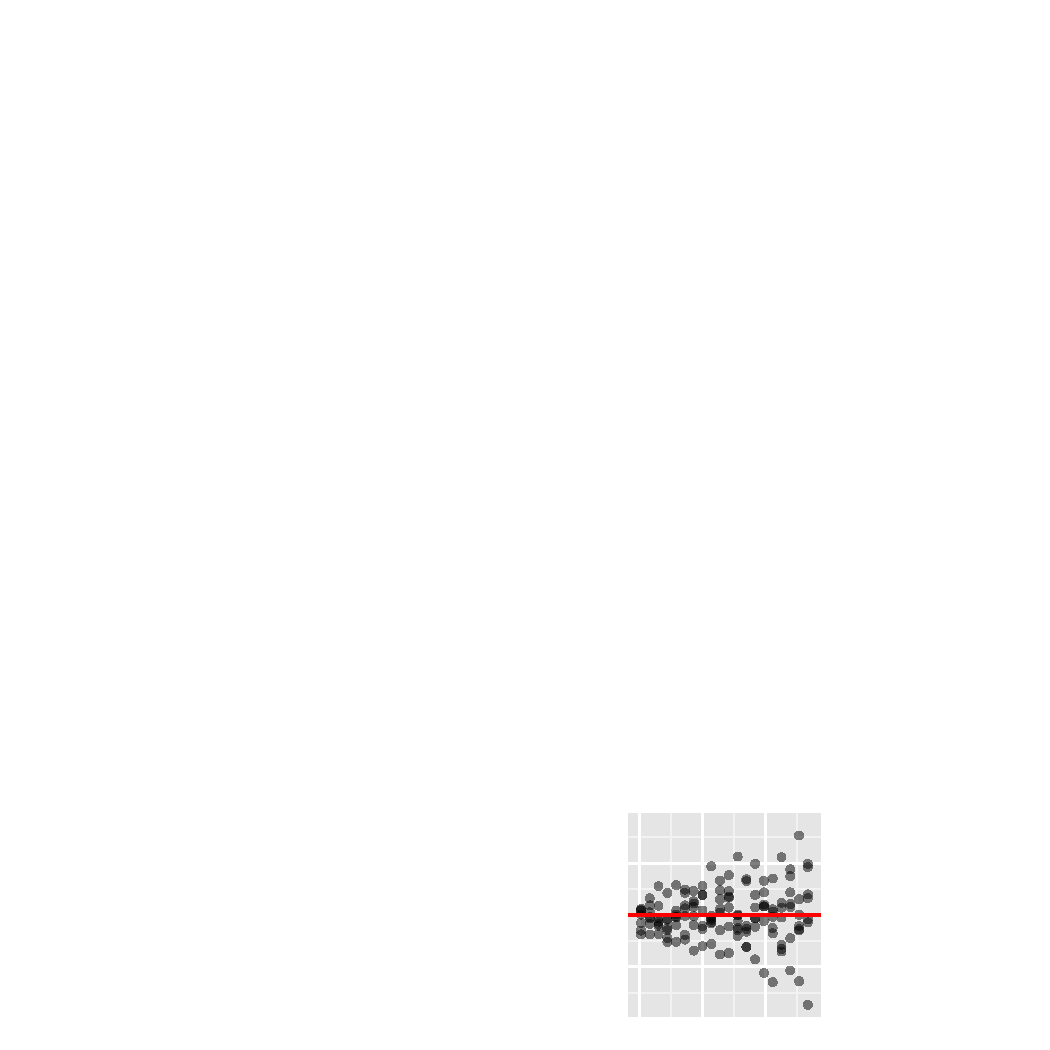
\includegraphics[width=0.05\textwidth]{homogeneous-dots-icon} & fig.~\ref{homogeneous-1}& 0/57 & \hspace{-0.1in}  & 1/71 & \hspace{-0.1in}  & 8/75 & \hspace{-0.1in}  & 0/59 & \hspace{-0.1in}  & 2/68 & \hspace{-0.1in}  & 0.7078 \\ 
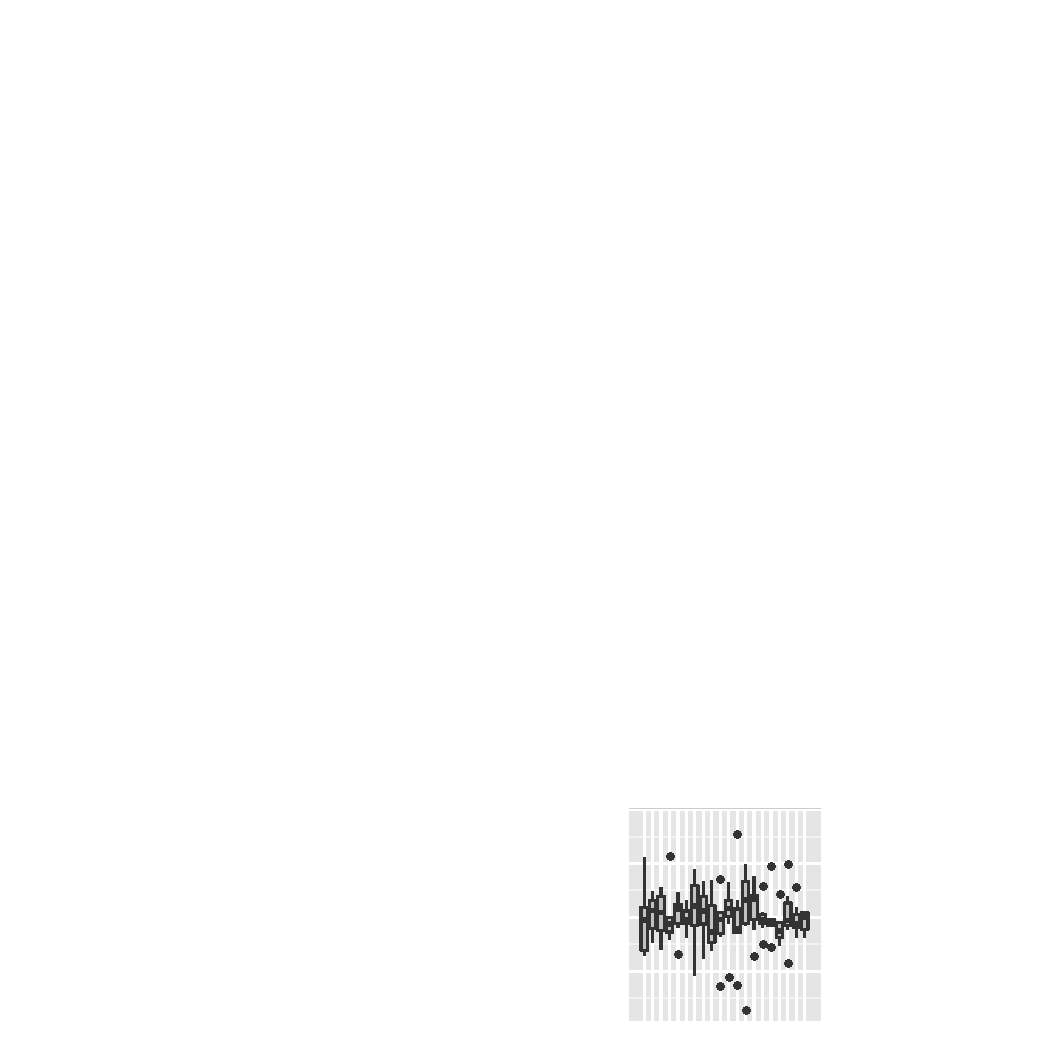
\includegraphics[width=0.05\textwidth]{homogeneous-bp-icon} &  fig.~\ref{homogeneous-2}& 23/61 & \hspace{-0.1in}*** & 38/72 & \hspace{-0.1in}*** & 29/59 & \hspace{-0.1in}*** & 22/70 & \hspace{-0.1in}*** & 35/62 & \hspace{-0.1in}*** & $<10^{-5}$\\ 
%
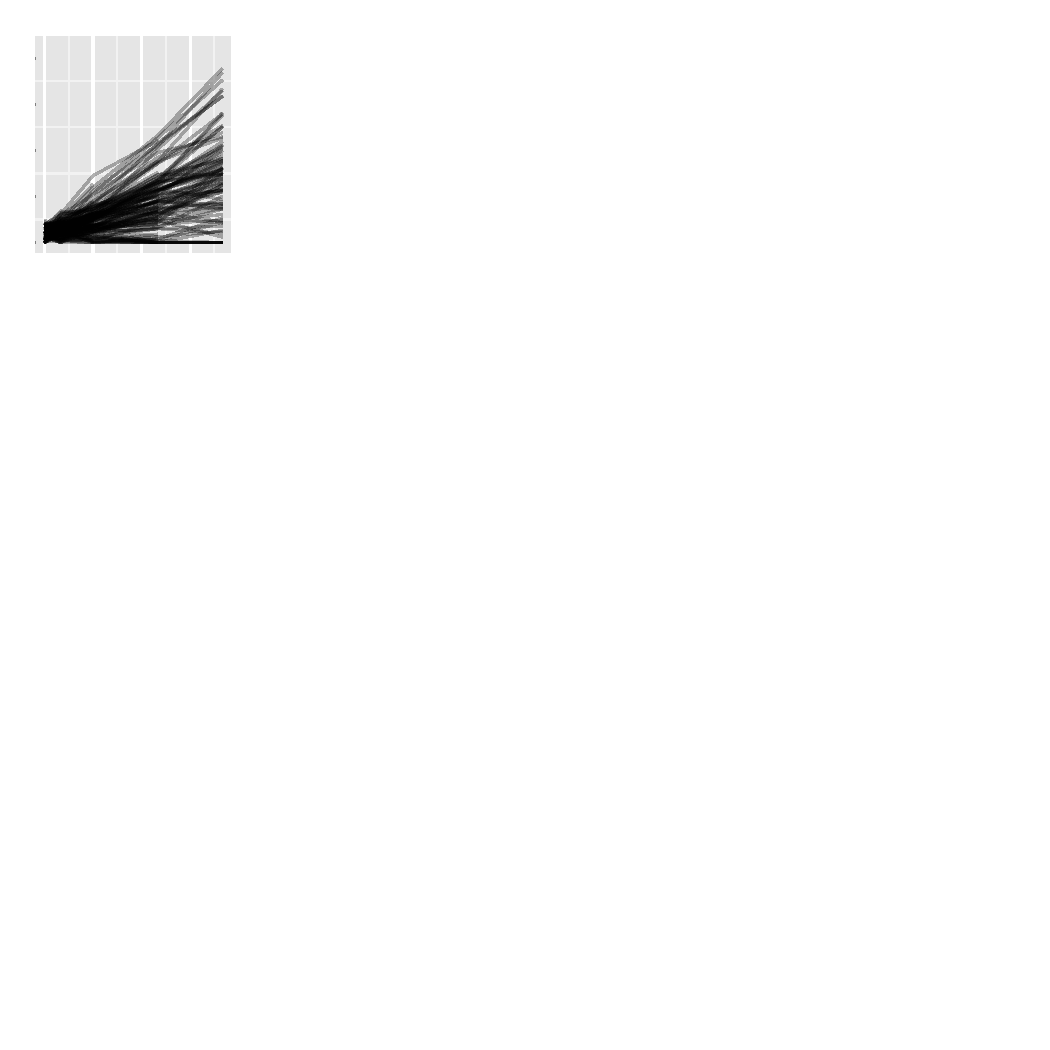
\includegraphics[width=0.05\textwidth]{autism2-fanned-icon}&   fig.~\ref{fig:autism-ranef} & 50/79&\hspace{-0.1in}***  & 26/59&\hspace{-0.1in}*** & 31/67&\hspace{-0.1in}*** & 32/72&\hspace{-0.1in}*** & 35/71&\hspace{-0.1in}*** & $<10^{-5}$\\ 
   \hline
\multicolumn{12}{l}{Signif. codes:  0 $\le$ *** $\le$ 0.001 $\le$ ** $\le$ 0.01 $\le$ * $\le$ 0.05 $\le$ . $\le$ 0.1 $\le$ ' ' $\le$ 1}

\end{tabular}
\end{table}



% latex table generated in R 3.1.1 by xtable 1.7-3 package
% Fri Aug 29 22:42:40 2014
\begin{table}[ht]
\caption{\label{tab:reasons} Percent of data picks given reason for the choice of plot from the lineup. }
\centering
\begin{tabular}{Mrrrrrrr}
  \hline
\multicolumn{2}{c}{Lineup} & Outlier & Spread & Trend & Asymmetry & Other \\ 
  \hline

\includegraphics[width=0.05\textwidth]{examfanned-icon} &  fig.~\ref{fig:fanned}  & 13.5 & 24.0 & 10.9 & 5.8 & 15.9 \\ 
 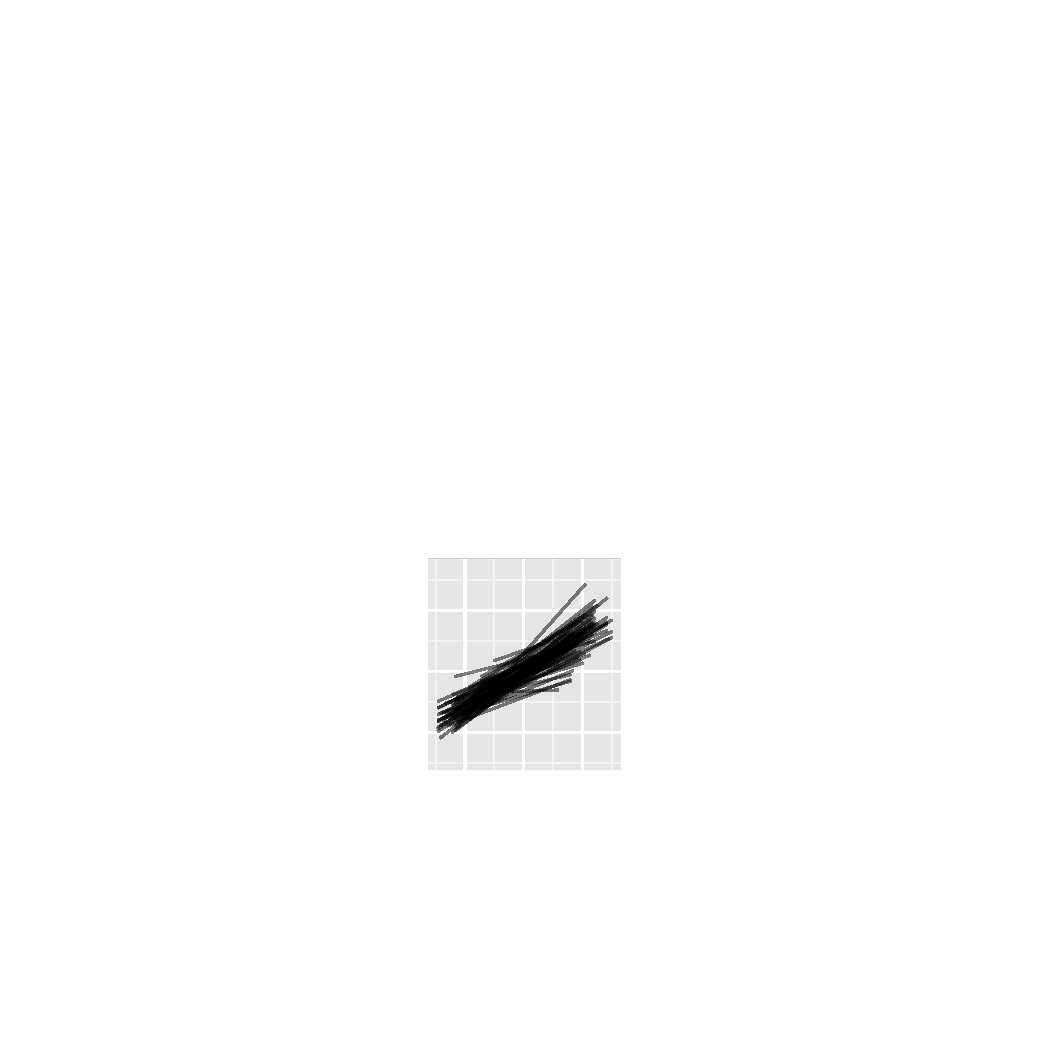
\includegraphics[width=0.05\textwidth]{exam-with-slope-icon} & fig.~\ref{fig:fanned2} & 2.4 & 10.6 & 3.5 & 5.4 & 0.0 \\ 

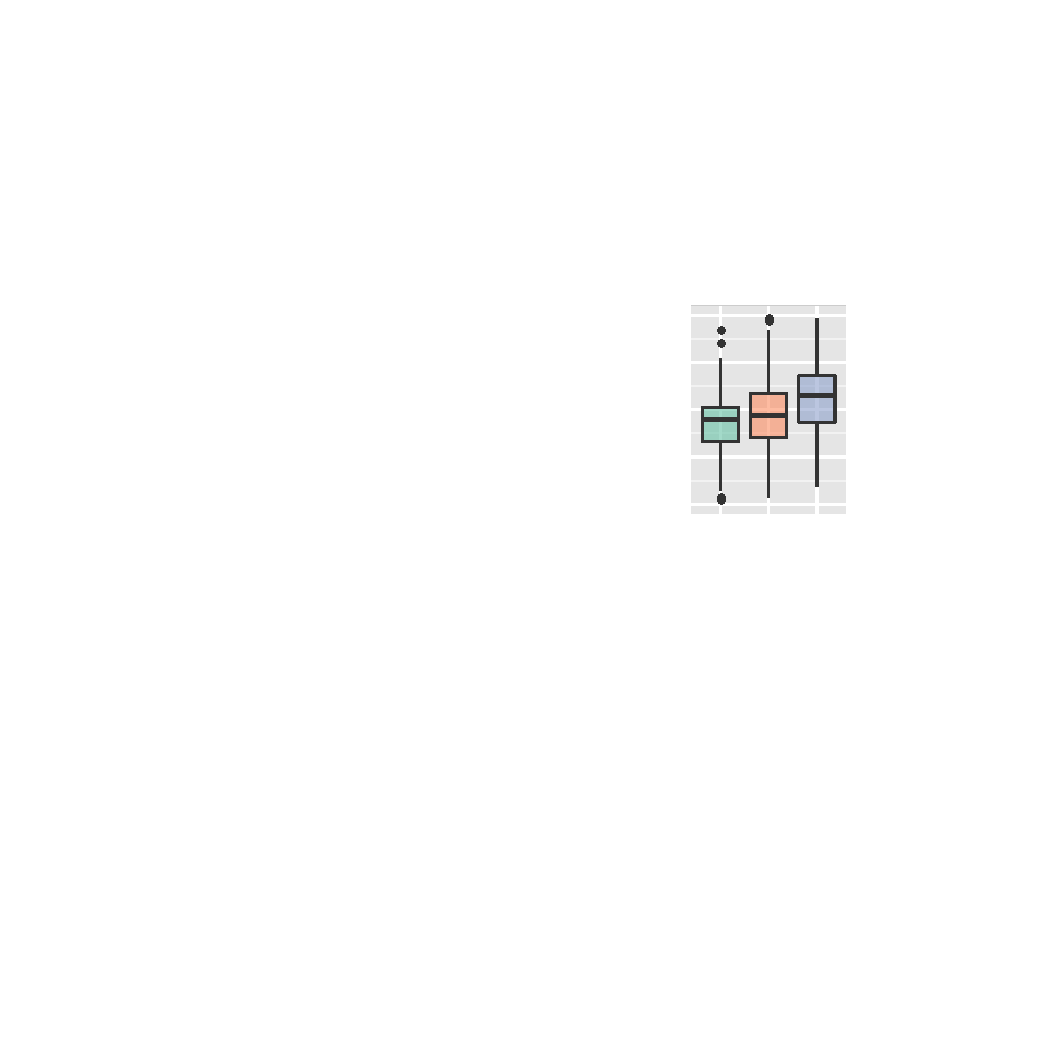
\includegraphics[width=0.05\textwidth]{autism-ordered-icon} &   fig.~\ref{fig:boxplot-ordered} & 73.3 & 95.5 & 92.5 & 91.0 & 80.7 \\ 
%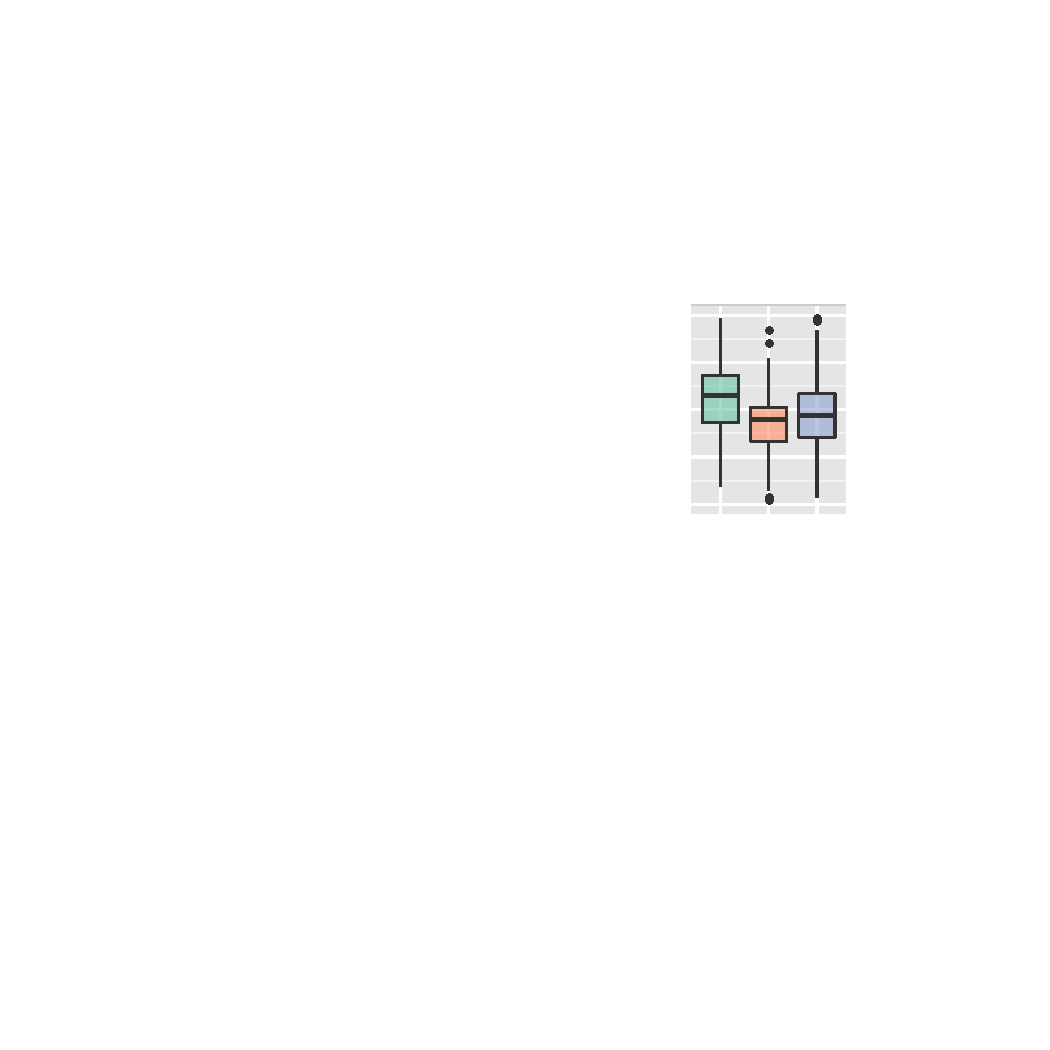
\includegraphics[width=0.05\textwidth]{autism-unordered-icon}&   fig.~\ref{fig:boxplot-unordered} & 80.2 & 99.5 & 92.4 & 91.2 & 86.2 \\ 

 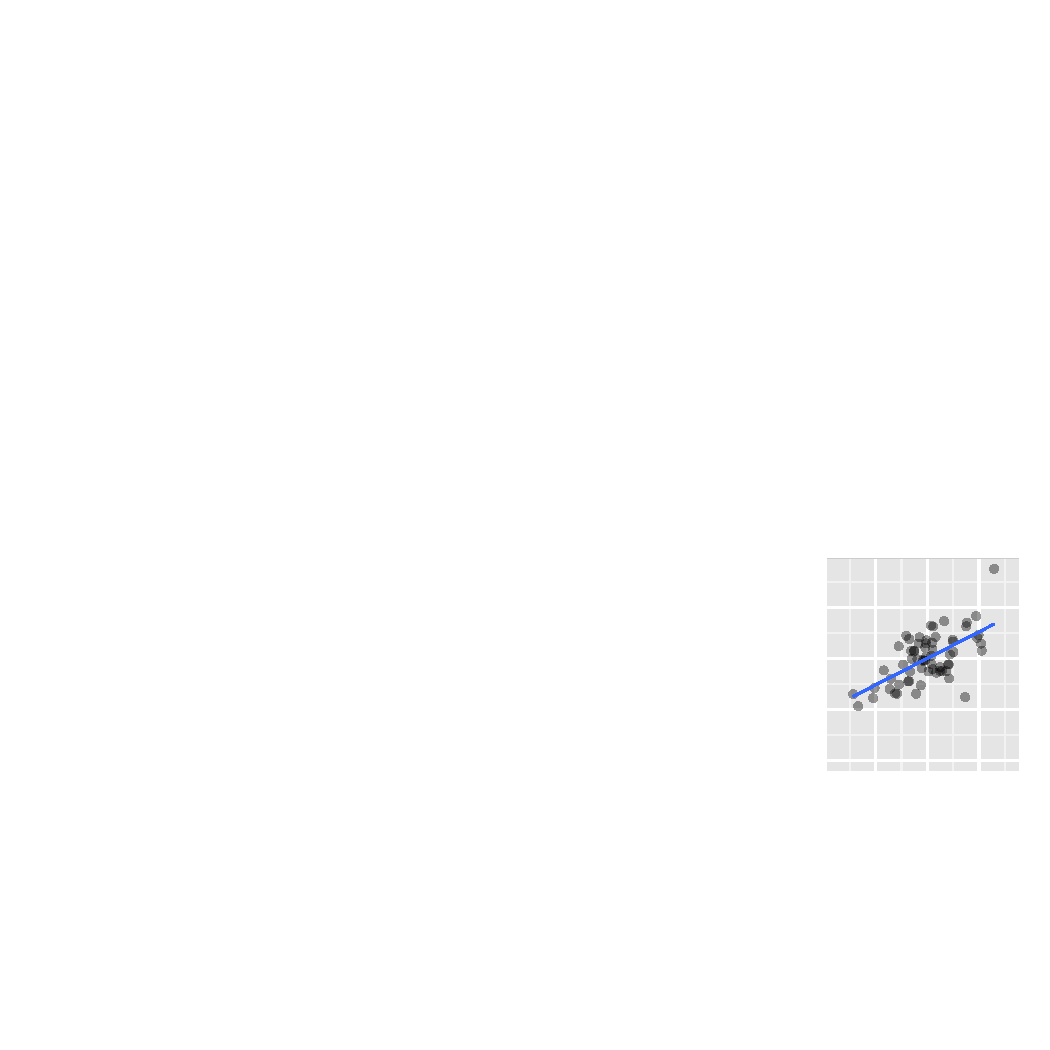
\includegraphics[width=0.05\textwidth]{examcorr-icon}&   fig.~\ref{fig:ranef-corr} & 64.5 & 34.3 & 83.4 & 70.7 & 64.9 \\ 

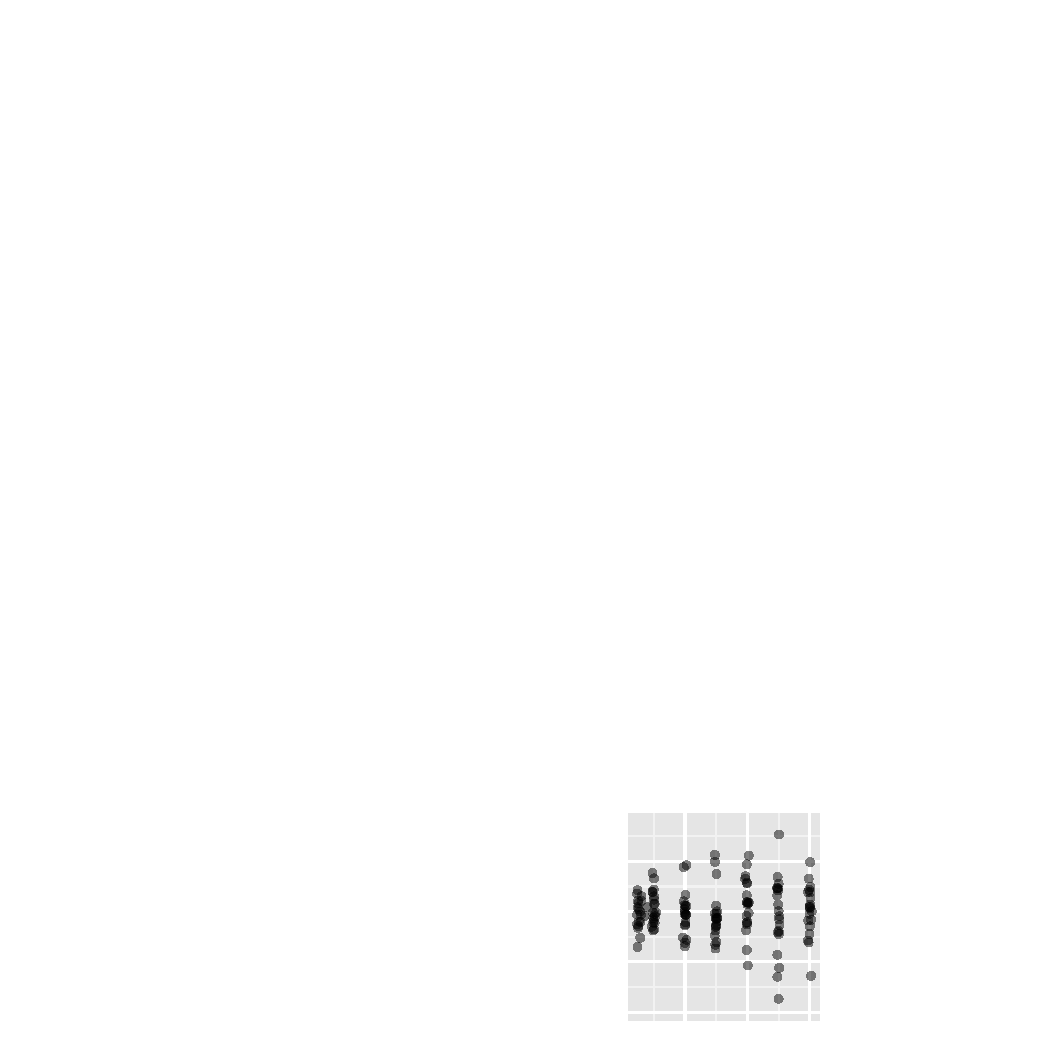
\includegraphics[width=0.05\textwidth]{dialyzerheterogeneous-icon}& fig.~\ref{fig:constvar2} & 18.8 & 27.0 & 29.1 & 25.8 & 19.0 \\ 
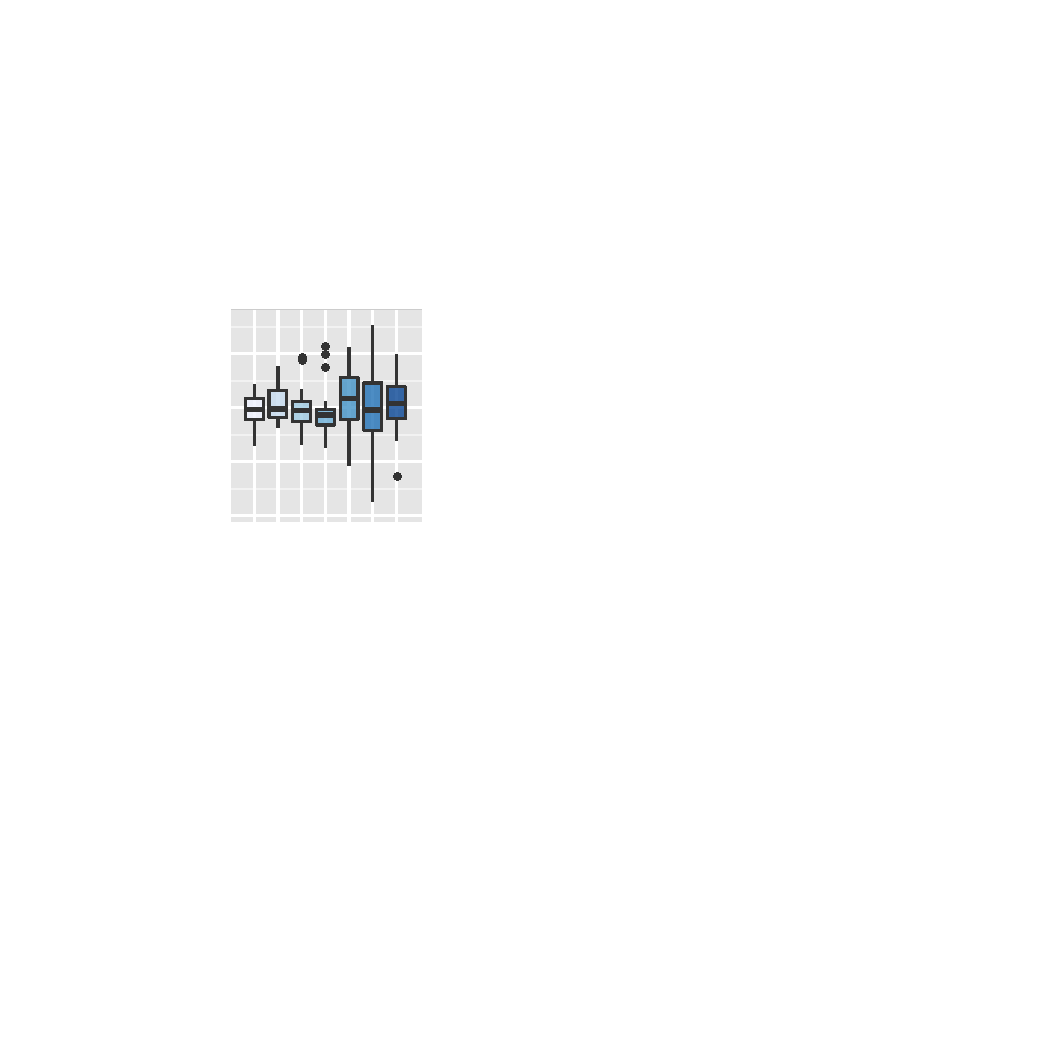
\includegraphics[width=0.05\textwidth]{dialyzerheterogeneous-bp}& fig.~\ref{fig:constvar2.bp} & 26.7 & 24.6 & 30.1 & 43.7 & 0.0 \\ 


\includegraphics[width=0.05\textwidth]{cyclone-icon}&   fig.~\ref{fig:badcyclone}  & 49.6 & 50.0 & 77.8 & 79.4 & 91.8 \\ 
\includegraphics[width=0.05\textwidth]{cyclone-good-icon}&   fig.~\ref{fig:goodcyclone}  & 4.2 & 0.6 & 2.4 & 6.7 & 0.0 \\ 

\includegraphics[width=0.05\textwidth]{dialyzernonlinear-icon}&   fig.~\ref{fig:linearity} & 84.0 & 87.4 & 98.3 & 98.1 & 100.0 \\ 
%  turk11-electoral & 14.9 & 15.4 & 10.8 & 27.3 & 12.7 \\ 
%  turk11-examuncorr & 21.8 & 24.5 & 21.3 & 7.0 & 7.7 \\ 

\includegraphics[width=0.05\textwidth]{radontranef-icon}&   fig.~\ref{fig:qqlineup-t} & 37.8 & 49.2 & 19.6 & 4.4 & 10.9 \\ 
\multicolumn{2}{r}{random intercept} & 1.5 & 0.0 & 1.1 & 0.0 & 0.0 \\ 
\multicolumn{2}{r}{random slope} & 0.0 & 0.0 & 0.0 & 0.0 & 0.0 \\ 
 \includegraphics[width=0.05\textwidth]{homogeneous-dots-icon} & fig.~\ref{homogeneous-1} & 2.4 & 3.0 & 7.6 & 4.8 & 0.0 \\ 
 \includegraphics[width=0.05\textwidth]{homogeneous-bp-icon} & fig.~\ref{homogeneous-2} & 56.8 & 55.1 & 20.1 & 33.9 & 22.7 \\ 
\includegraphics[width=0.05\textwidth]{autism2-fanned-icon}&   fig.~\ref{fig:autism-ranef}  & 38.9 & 33.8 & 56.8 & 78.5 & 70.0 \\ 
   \hline
\end{tabular}
\end{table}


%------------------------------------------------------------------------------------
\subsection{Additional lineups included in the study}\label{app:morelineups}
%------------------------------------------------------------------------------------

This section includes two lineups that were included in the  MTurk study, but were not discussed in the paper. 

Figure~\ref{fig:constvar2.bp} contains a box plot representation of the same data as Figure~\ref{fig:constvar2}, with the  difference that pressure is categorized into seven categories, and residuals are shown in the form of box plots. In order to preserve the appearance of continuity on the $x$-axis we have used a color scheme to fill the boxes with deepening shades of blue from left to right. In this form 23 out of 70 observers identify the plot of the data.  This is consistent with the other design.

\begin{figure}[hbt]
	\centering
	\includegraphics[width=0.8\textwidth]{dialyzerheterogeneous-bp-19.pdf}
	\caption{\label{fig:constvar2.bp} 
	Alternative box plot  Lineup testing homogeneity of the level-1 residuals. Which of the plots is the most different? Which feature led you to your choice?}
%	Lineup of 20 scatterplots of level-1 residuals against pressure used to test the assumption of homogeneous level-1 residual variance for the dialyzer study.  Which is the real plot?}
\end{figure}


%%%%%%%%%%%%%%%%%%%




%\hhnote{reference to corresponding lineup in main paper}
Figure~\ref{fig:autism-ranef} displays another lineup testing the adequacy of the random effects specification  (see section~\ref{sec:random}) using data from the autism study. The null plots were generated from a model containing only a linear random slope, so if the true plot in panel \#($\sqrt{16} + 12$) is identified it provides support for the inadequacy of this specification, and need for additional random effects. %Figure~\ref{fig:boxplot-unordered} shows similar data  as Figure~\ref{fig:boxplot-ordered}, where categories were re-labelled to investigate whether the order might have an effect on people's choices. Interestingly, the power is the same, and observers still identify 'trend' as one of the top reason for their choice.

\begin{figure}
	\centering
	\includegraphics[width=0.8\textwidth]{autism-fanned2-16.pdf}
	\caption{\label{fig:autism-ranef} Which of the plots is the most different? Which feature led you to your choice? }
\end{figure}

%\begin{figure}[h]
%	\centering
%	\includegraphics[width=0.8\textwidth]{autism2-unordered-10.pdf}
%	\caption{\label{fig:boxplot-unordered} An alternative layout of Figure~\ref{fig:boxplot-ordered}, where the boxplots are ordered as they are for inference. Which of the plots is the most different? Which feature led you to your choice?}
%\end{figure}

%%%%%%%%%%%%%%%%%%%


\begin{figure}[hbt]
	\centering
	\includegraphics[width=0.8\textwidth]{dialyzerhomogeneous-dots-1-19.pdf}
	\caption{\label{homogeneous-1}
	Lineup testing homogeneity of the level-1 residuals. Which of the plots is the most different? Which feature led you to your choice?}
%	Lineup of 20 scatterplots of level-1 residuals against pressure used to test the assumption of homogeneous level-1 residual variance for the dialyzer study.  Which is the real plot?}
\end{figure}
\begin{figure}[hbt]
	\centering
	\includegraphics[width=0.8\textwidth]{dialyzerhomogeneous-1-19.pdf}
	\caption{ \label{homogeneous-2}
	Lineup testing homogeneity of the level-1 residuals. Which of the plots is the most different? Which feature led you to your choice?}
%	Lineup of 20 scatterplots of level-1 residuals against pressure used to test the assumption of homogeneous level-1 residual variance for the dialyzer study.  Which is the real plot?}
\end{figure}


%\alnote{Figures~\ref{homogeneous-1} and~\ref{homogeneous-2} are really no different from the cyclone plots, aside from showing two different designs. I am not sure whether they add anything to the discussion in this section. To me they seem to detract from the cyclone plot discussion. One idea is to move them to the appendix where we can highlight the difference in designs. I don't think moving this would detract from how ``novel'' our contribution is.}

Figures~\ref{homogeneous-1} and~\ref{homogeneous-2} show another example of testing for homogeneity in the variance following the approach taken in section~\ref{sec:homogeneity}. Both of these lineups are based on the dialyzer data. 
%\alnote{I am confused by plots 7 and 8. What data set are they displaying?}

Level-1 residuals are plotted by subject. Subjects are ordered by variance, i.e.~we get some structure that might be taken for differences in variability, that are really just differences due to the imbalance in group size. If any panel of this lineup is considered separately, an analyst may come to the conclusion that the within-group variance increases across the $x$ axis.  However, inserting the true plot into the lineup forces the analyst to consider this particular feature as inherent to the data structure rather than evidence against a hypothesis of homogenous variance. 
The dot plot version is not significant, but the box plot version is. When participants in the box plot design identify the data plot, about 45.3\% give outliers as the reason for their choice. In contrast to that, outliers, a large spread or a trend are in a three-way tie for the reason for identifying the data plot in the lineup with the dot plot design.
%Outliers       Large spread       Trend       Asymmetry       Other
% dialyzerhomogeneous
%  correct        1        2        3        4        5
%1   FALSE 38.86852 33.89209 13.35778 12.46726 1.414353
%2    TRUE 25.35211 28.16901 29.57746 16.90141       NA
% dialyzerhomogeneous-bp
%  correct        1        2        3        4        5
%1   FALSE 29.09350 25.72378 28.286664 12.05505 4.841006
%2    TRUE 45.31162 37.28243  8.422235  7.29927 1.684447

The reason for the box plot design being so much more significant might not be so much of an issue of homogeneity being violated as much as a difference in the error distribution between the data and the nulls. Null data come from a parametric bootstrap where residuals are simulated under a normal error assumption. Outliers in small samples are indicative of the sample being from a distribution with heavy tails.
Regardless of the reasoning, the second lineup design enables us to diagnose a problem with the model that makes the data stand out from a set of nulls.  The two designs therefore represent two very similar tests with different power.


%%%%%%%%%%%%%%%%%%%


\end{document}


\dcnote{Can we take out everything from here through to the start of visual inference, and begin the paper with the material in the ``linear mixed effects models'' section?} Statistical modeling involves a cyclical process consisting of exploration, estimation, and validation. When a structure of interest is identified in the data we model this relationship, take it out of the data, and search the residuals for additional structure that is yet unexplained; thus, exploratory and confirmatory methods in statistical modeling are inherently linked \citep{tukey:eda}.
%Valid model-based statistical inference relies on proper specification of a model, making diagnostic tools central to the analytic process. 
Graphical methods are commonly used in model validation \citep{GelmanHill:2007}. Depending on methodology, different diagnostics are suggested for assessing distributional assumptions and assessing model fits in detail. In the linear model setting, Quantile-Quantile (Q-Q) plots and scatterplots with smoothers are often used \citep{Cook:1999}. In the Bayesian framework, \citet{Gelman:2004gg} proposes simulation from posteriors to assess goodness-of-fit. 
%In the Bayesian framework simulation from the posterior predictive distribution have been proposed to assess goodness-of-fit, which can displayed graphically \citep{Gelman:2004gg}. 
While the use of statistical graphics is wide-spread in exploratory data analysis and informal validation, graphics are often considered to be too subjective to be the sole basis for model selection or validation. 
At the core of this criticism is the fact that decisions are  based on a single plot. With only a single plot,  the detection of any unexpected structure leads to the conclusion that the model is inappropriate; however, in complex models we often observe structure 
%artificial structures are often observed 
in the residuals, even when models are properly specified \citep[c.f.,][]{Morrell:2000ve, Gelman:2000dr}. 
These drawbacks lead to an over-reliance on conventional hypothesis tests %for model selection and validation 
for complex models where such procedures often perform sub-optimally.

%however, conventional practices for the selection and validation of linear mixed-effects models often rely on test statistics with questionable reference distributions and residual plots that exhibit artificial structure in well-fitting models. Graphical displays are often suggested 
%
%Recently, visual simulation-based diagnostics \citep{Gelman:2004gg} and inference \citep{Buja:2009hp} have been formulated, providing a rigorous framework for graphical discovery. Instead of relying on adjustments to reference distributions that must be considered on a case-by-case basis, we propose utilizing the framework of visual inference \citep{Buja:2009hp, mahbub:2013} as a unified graphical approach that harnesses our innate abilities to detect extremes to overcome such problems. This approach is able to enhance familiar statistical graphics from linear models, such as Quantile-Quantile (Q-Q) plots and scatterplots with smoothers, to avoid the detection of artificial structures. 

%Statistical modeling involves a cyclical process consisting of exploration, estimation, and validation. When a structure of interest is identified in the data we model this relationship and look past this structure in search of additional structure that is unexplained by the model; thus, exploratory and confirmatory methods in statistical modeling are inherently linked. While there is a wide-spread use of graphical methods for exploration, they are often deemed too subjective to be the sole basis for model selection or validation. This viewpoint leads to an over-reliance on conventional hypothesis tests 
%%for model selection and validation 
%in complex models where such procedures often perform sub-optimally.
%Until now, when such situations were encountered an analyst was forced to either accept the approximate results offered by conventional hypothesis tests or appeal to simulation via the parametric bootstrap to adjust results \citep[c.f.,][]{Longford:2001wy}. 
%\todo[inline]{what makes the parametric bootstrap solution unsatisfactory? -- we shouldn't bring it up unless there's a good reason to not use it. }
%\alnote{I refer to the fact that they require more computation time than the lineups later in the paper. Also, like classical hypothesis tests, they only provide decisions whereas lineups provide additional information.}
Recent developments in graphics methodology provide a rigorous framework for graphical discovery: visual inference  \citep{Buja:2009hp}  allows for the quantification of the significance of graphical findings. In simulation-based studies visual inference has been shown to perform similarly to classical tests  \citep{mahbub:2013}. Using visual inference, we suggest and validate a framework
 that enables us 
 to overcome common difficulties  with conventional hypothesis tests 
% and statistical graphics 
 %that are encountered 
 in the selection and validation of linear mixed-effects models. 
% This approach is able to enhance familiar statistical graphics to avoid the detection of artificial structures. 



%In this paper we apply the  framework of visual inference  \cite{Buja:2009hp, mahbub:2013} to address common difficulties encountered in the selection and validation of linear mixed-effects (LME) models.

%Visual inference provides a unified graphical approach to account for such problems encountered with complex models while relying on familiar statistical graphics. 

In order to develop such graphical tools as complements to conventional tests, we must first define the inferential framework on which we rely.

%\alnote{Do we need more of a transition here? When I was reading this I realized this was the end of the ``general introduction'' and the following sections introduce specific topics/issues. Would it make sense to go back to subheadings?}
%\hhnote{subheadings will be a bit tricky at the end of the introduction, when we are going into the purpose of the paper - but if you have good ideas, go ahead with the subheadings.}